
\documentclass[
    11pt, % The default document font size, options: 10pt, 11pt, 12pt
%oneside, % Two side (alternating margins) for binding by default, uncomment to switch to one side
    english, % ngerman for German
    oneside
]{book} % The class file specifying the document structure

\usepackage{setup} % preamble with commands
\usepackage{theorems}
\usepackage{commands}

% Define Document Variables
% Variables
\def\notetitle{CLIMATE SYSTEM MODELING}
\def\noteauthor{
    \textbf{Professor} Antonio Navarra \\
    by Niccolò Zanotti\\
    University of Bologna\\
    Updated \today}
\def\notedate{2024/2025}

% ------------------------------------------------------------------------------

\begin{document}
    \title{\textbf{
        \LARGE{\notetitle} \vspace*{10\baselineskip}}
    }
    \author{\noteauthor}
    \date{\notedate}

    \maketitle
    \newpage

    \tableofcontents
    \newpage

% ------------------------------------------------------------------------------

    \section{Introduction}\label{introduction}

Sample citation of \citet{Richardson1922}.

The atmosphere is in motion and it is a continuous mixing and clashing
of vortices and structures, but when it is averaged over a long period
of time (\fig{\ref{fig:ERA5-wind200}}) it shows a remarkable simple structure.
The figure shows the wind at an approximate level of about 12km, that is
considered to be in the free atmosphere, far from the influence of the
ground. The circulation is a large vortex around the pole that shows
small oscillation in latitudes, especially pronounced over North America
and the Asian Pacific Coast. The flow is therefore predominantly in the
East-West direction, with a relatively small component in the meridional
direction. The \emph{circumpolar vortex} has been one of the first
structures to be recognized when plentiful observations of the upper air
flow became available, but it provided some of the intriguing questions
that drove the development of geophysical fluid dynamics to this time.
some of them have not been completely understood. What is maintaining
this peculiar circulation ? Which factor determines the amplitude and
location of the undulations in meridional direction ? Some of these
question will be addressed in these notes

\begin{figure}
\centering
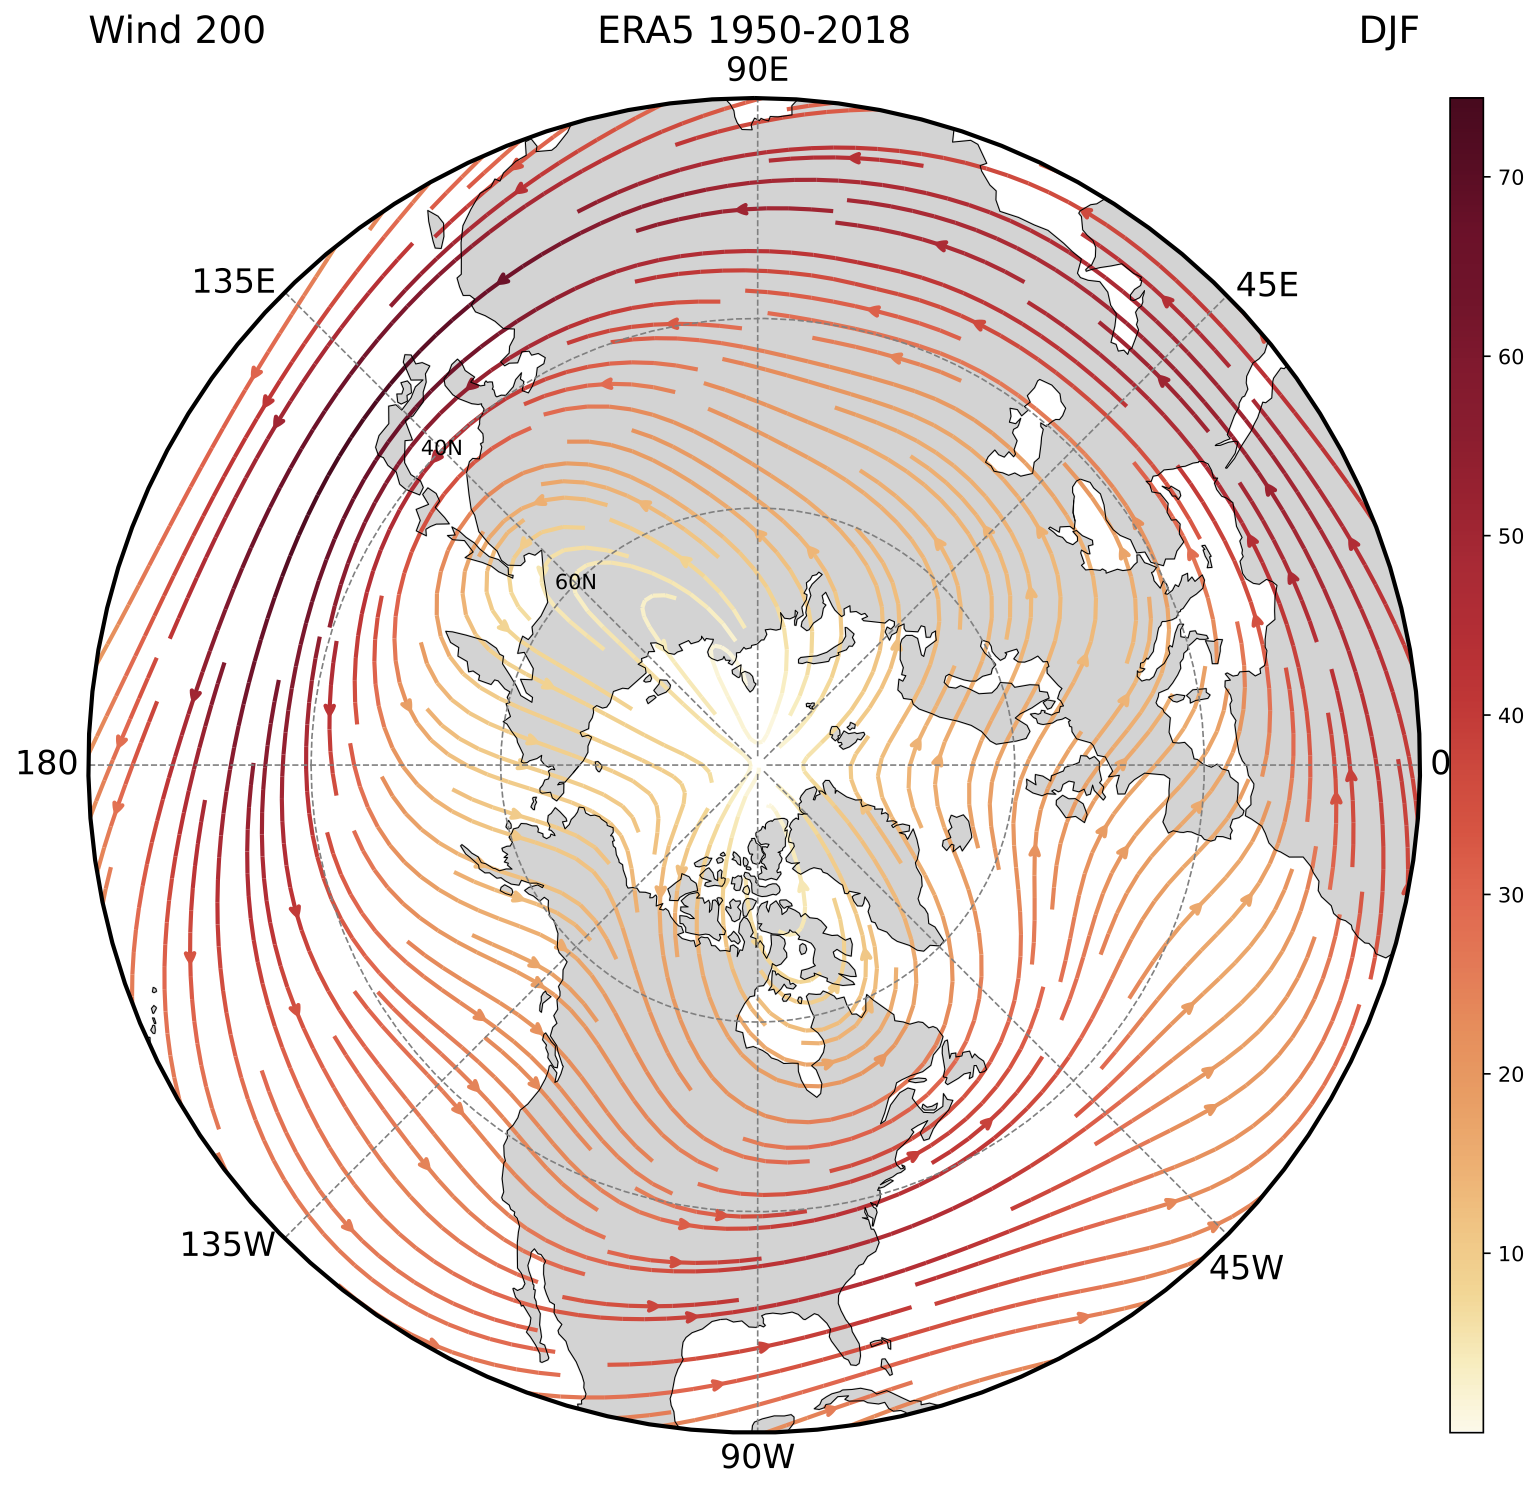
\includegraphics[width = .7 \textwidth]{figs/GD/Wind200.png}
\caption{}
\label{fig:ERA5-wind200}
\end{figure}


\subsection{Coordinate systems}\label{coordinate-systems}

\subsubsection{Spherical Coordinates}\label{spherical-coordinates}

The most commonly used coordinate system for the analysis of the
atmosphere and the oceans is a spherical coordinate system attached to
the rotating Earth (Fig. \texttt{fig:0} ). The spherical coordinates are
slightly different from the usual mathematical ones as the latitude is
measured from the equator and therefore it can take negative values. The
longitude is running west to east.

The longitude is also known as the ``zonal'' direction whereas the
latitude is also known as the "meridional" direction. Winds are
identified by the direction they are coming from, so a "westerly" wind
is coming \emph{from} the West and an "easterly" wind is coming from the
East.

This coordinate system is rotating with the Earth and therefore it
generates force terms in any dynamical equation expressed in this system
of coordinate, the Coriolis terms.

\begin{figure}
\centering
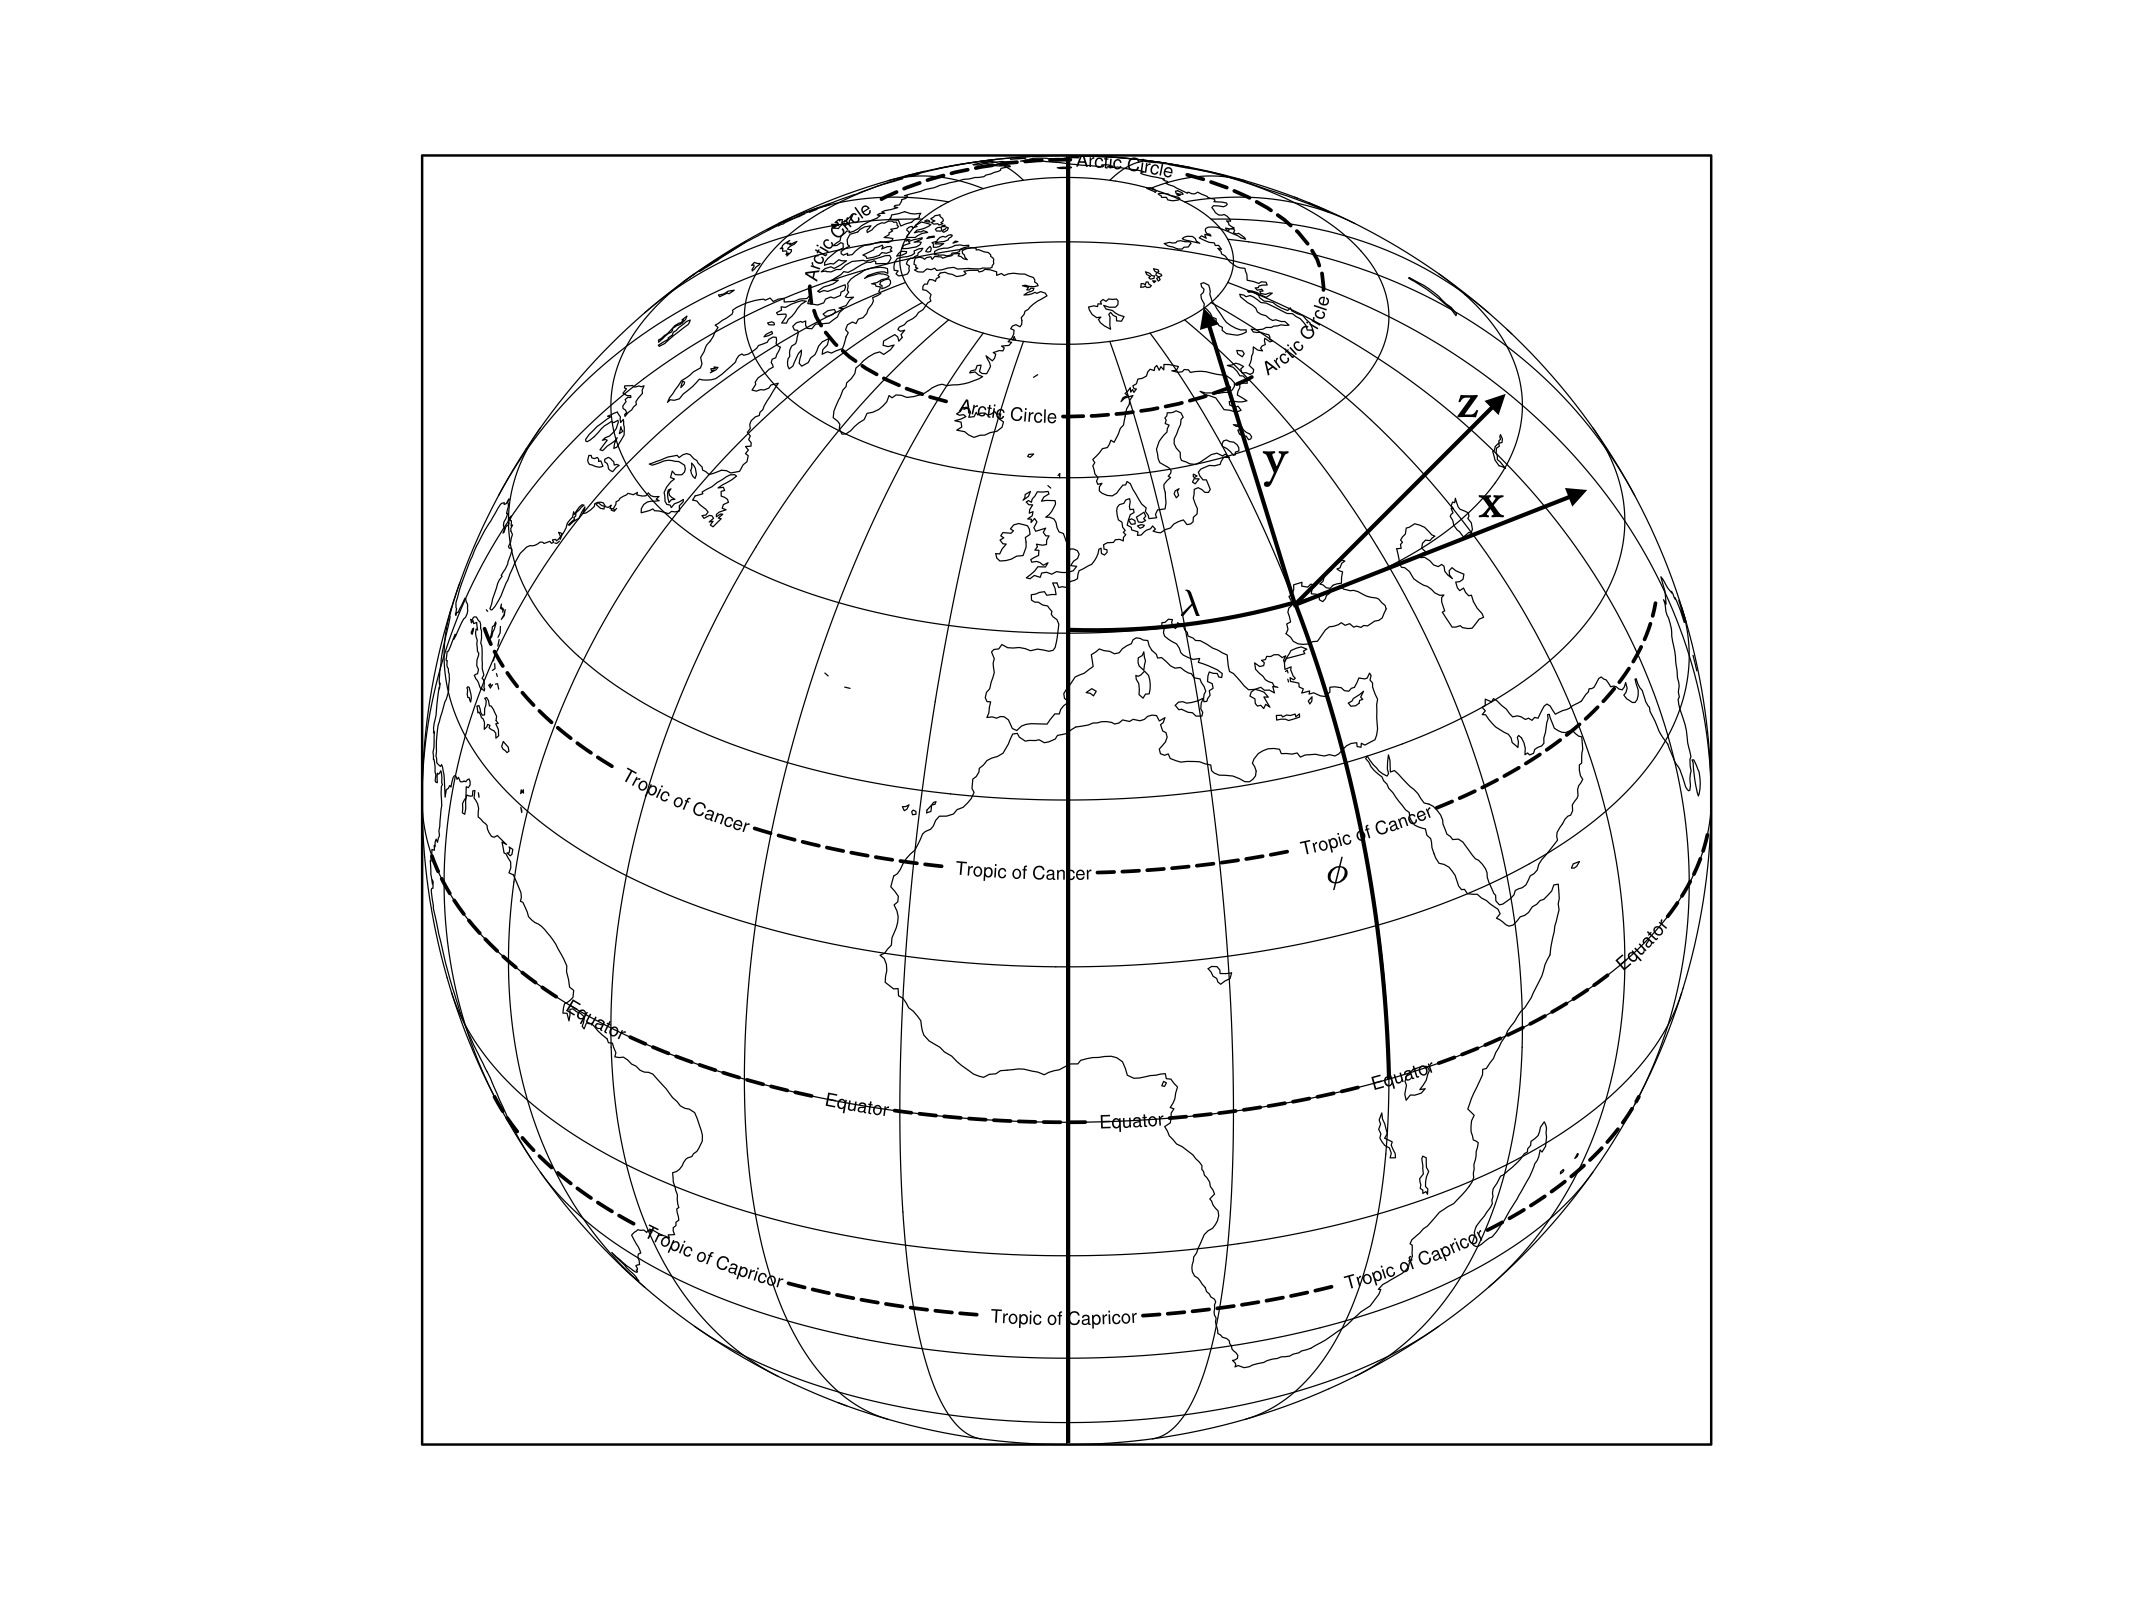
\includegraphics[width = .7 \textwidth]{figs/GD/map.png}
\caption{Coordinate System}
\label{fig:3d-coordinate-system}
\end{figure}

\subsubsection{The Beta-plane}\label{the-beta-plane}

It is sometimes convenient to shift coordinate system if the latitudinal
extension of the motion is not too great with respect to the motion
parameters as they are expressed in the adimensional numbers. When this
is possible, a tangent coordinate system is applied at a specific
latitude \(\phi_0\) and the resultant Cartesian coordinates system is
called the \(\beta\)-plane. Usually symbols \((x,y)\) are used in this
case for the zonal and meridional coordinate. In the \(\beta\)-plane the
planetary vorticity \(f\) is linearized as \(f=f_0 + \beta y\), where
\(\beta = \frac{\partial f}{\partial y}({\phi_0})\).

\subsection{Advective derivative}\label{Sec:Adv}

To describe the governing equation of the atmosphere and eventually of
the ocean we have to understand how we write the rate of change with
time of this fluid. This problem was solved by considering the fact that
the rate of change in the fluid cannot be seen as arate of change with
respect to a fixed system of coordinate because the system is moving
with the fluid itself. Therefore, first we have to find a way to
describe the change taking into account the moving system of
restaurants. These can be done by using a concept developed in the 19th
century by Euler that is called "advective derivative" that can be
obtained from a total derivative of the property,

\[\frac{d \phi}{dt} = \frac{\partial \phi}{\partial t} + \frac{\partial x}{\partial t}\frac{\partial \phi}{\partial x} + \frac{\partial y}{\partial t}\frac{\partial \phi}{\partial y}+\frac{\partial z}{\partial t}\frac{\partial \phi}{\partial z} = \frac{\partial \phi}{\partial t} + \mathbf{v}\cdot\nabla\phi\]

and so it can be defined as

\[\frac{D \varphi}{Dt} =\frac{\partial \varphi}{\partial t} + \mathbf{v}\cdot\nabla\varphi\]

in this way the moving fluid can be described by derivatives with
respect the "fixed" coordinate system, i.e. the Eulerian description.
The alternative description of the observer moving with fluid is known
as the "Lagrangian" description.

\subsection{Primitive Equations}\label{Sec:Prim}

The equation governing the motion of the atmosphere can be written as:

\[\begin{aligned}
&\frac{D u}{Dt} -\frac{uv \tan{\phi}}{r} +  \frac{uw}{r} = -\frac{1}{\rho r \cos{\phi}}\frac{\partial p}{\partial \lambda} + fv - \hat{f}w + F_\lambda\\
&\frac{D v}{Dt} -\frac{u^2 \tan{\phi}}{r} +  \frac{vw}{r} = -\frac{1}{\rho r }\frac{\partial p}{\partial \phi} - fu  + F_\phi\\
&\frac{D w}{Dt} -\frac{u^2+v^2}{r} = -\frac{1}{\rho }\frac{\partial p}{\partial z} -g +\hat{f}u + F_z\\
\end{aligned}\]

the \(f=2\Omega \sin{\phi}\) and \(\hat{f} = 2\Omega\cos{\phi}\) terms
arise from the rotating spherical coordinate system that we have chosen,
other terms are generated by the spherical geometry. Some of them are
small and traditionally they can be neglected, so that we arrive at the
system

\[\begin{aligned}
&\frac{D u}{Dt} - v\left(f +  \frac{u \tan{\phi}}{a}\right)  = -\frac{1}{\rho a \cos{\phi}}\frac{\partial p}{\partial \lambda}   + F_\lambda\\
&\frac{D v}{Dt} + u\left( f + \frac{u \tan{\phi}}{a}\right)  = -\frac{1}{\rho a}\frac{\partial p}{\partial \phi}  + F_\phi\\
&\frac{D w}{Dt}  = -\frac{1}{\rho }\frac{\partial p}{\partial z} -g  + F_z\\
\end{aligned}\]

where we have also used the \emph{Shallowness Approximation} by assuming
\(r = a +z \approx a\), where \(a\) is the Earth radius.

However the advective derivative must be expressed in spherical
cordinates

\[\frac{D }{Dt} = \frac{\partial }{\partial t} + \frac{u}{a\cos{\phi}}\frac{\partial }{\partial \lambda} +\frac{v}{a}\frac{\partial }{\partial \phi} + w\frac{\partial }{\partial z}\]

so that the velocity components are

\[\begin{aligned}
&u = a\cos{\phi\frac{\partial \lambda}{\partial t}}\\
&v = a \frac{\partial \phi}{\partial t}\\
&w = \frac{\partial z}{\partial t}
\end{aligned}\]

These equation govern the mechanical behaviour of the atmosphere, and we
will see in a different form, also of the ocean. There three forces in
action: pressure gradient, rotaiton via the Coriolis force and gravity.

The equation are not complete,we have three equation but five variables,
so we need to find the missing relations. We are using the basic
conservation principles, the latter equations describe the conservation
of momentum, we can exploit the conservation of mass. The mass of the
fluid must be conserved locally, because there are now sinks or sources
in the atmosphere itself, so we want to write the mass of a volume of
atmosphere fixed in space as

\[M = \int_V  \rho \,dV\]

the mass in the volume can only change if there is a flux of mass at
surface \(S\),

\[\frac{\partial }{\partial t} \int_V  \rho \,dV = -\int_S \rho\mathbf{v}\cdot n \, dS\]

using the divergence theorem however we have

\[\frac{\partial }{\partial t} \int_V  \rho \,dV = -\int_V \nabla\cdot(\rho\mathbf{v}) \,dV\]

because the volume is not changing with time we can bring the derivative
inside the integral and we get

\[\int_V  \frac{\partial \rho}{\partial t}+\nabla\cdot(\rho\mathbf{v}) \,dV = 0\]

but the volume is arbitrary, so it must be that

\[\frac{\partial \rho}{\partial t}+\nabla\cdot(\rho\mathbf{v}) = 0\]

is valid locally.

We have still at our disposal the conservation of thermodynamical energy
and so we can also use

\[C_v\frac{D T}{Dt} = -p\frac{D }{Dt}\left(\frac{1}{\rho}\right)+ Q\]

where we included the temperature and heating/cooling term \(Q\). The
state variable are then linked by the state equation

\[p = \rho R T\]

where \(R\) is the gas constant for dry air.

We can use the equation of state to write the energy equation ( or the
temperature equation) in a different form,

\[c_v\frac{D T}{Dt} = -p\frac{D }{Dt}\left(\frac{R T}{p}\right)+ Q = -R\frac{D T}{Dt} + \frac{RT}{p}\frac{D p}{Dt} + Q\]

yielding the alternative forms ( since \(c_p = c_v +R\)),

\[c_p\frac{D T}{Dt}  - \frac{1}{\rho}\frac{D p}{Dt} = Q\]

For adiabatic processes \(Q=0\) and so

\[\begin{aligned}
&c_p\frac{D T}{Dt}  - \frac{1}{\rho}\frac{D p}{Dt} = 0\\
&\frac{c_p}{T}\frac{D T}{Dt} -\frac{R}{p}\frac{D p}{Dt} = 0\\
&\frac{D }{Dt}\log{T} - \frac{R}{c_p}\frac{D }{Dt}\log{p} = 0
\end{aligned}\]

integrating it we get

\[\log{T/T_0} - \log{\left(\frac{p}{p_0}\right)^{R/c_p}} = const\]

or

\[\frac{T}{T_0}\left(\frac{p_0}{p}\right)^{R/c_p} = const\]

so the quantity, known as \emph{potential temperature}

\[\theta = T\left(\frac{p_0}{p}\right)^{R/c_p}\]

is conserved in adiabatic processes and the thermodynamics equation can
be written as

\[\frac{D \theta}{Dt} = Q\]

\subsection{Hydrostatic balance}\label{hydrostatic-balance}

Under the action of gravity the vertical component of the pressure
gradient force balances the action of gravity, resulting in very small
vertical acceleration

\[\frac{\partial p}{\partial z} =  -g \rho\]

then if we take the vertical derivative of the eq. \texttt{Eq:logT}

\[\frac{1}{T_0}\frac{d T}{dz}\left(\frac{p_0}{p}\right)^{R/c_p} -\frac{p_0}{p^2}\frac{R}{c_p}\frac{T}{T_0}\left(\frac{p_0}{p}\right)^{R/c_p-1}\frac{d p}{dz} = 0\]

simplifying

\[\frac{d T}{dz} -\frac{p_0}{p^2}\frac{R}{c_p}T\left(\frac{p_0}{p}\right)^{-1}\frac{d p}{dz} = 0\]

or

\[\frac{d T}{dz} -\frac{1}{p}\frac{R}{c_p}T\frac{d p}{dz} = \frac{d T}{dz} +g\rho\frac{1}{p}\frac{R}{c_p}T = 0\]

but using the equation of state

\[\frac{d T}{dz} = -\frac{g}{c_p}\]

that gives how the temperature change with height under adiabatic
conditions and when the hydrostatic balance is valid. This is known as
the \emph{adiabatic lapse rate}.

\subsection{Summary of fundamental
equations}\label{summary-of-fundamental-equations}

Summarizing our discussion, the fundamental equation that describe the
motion of the atmosphere then are:

\[\begin{aligned}
&\frac{D u}{Dt} - v\left(f +  \frac{u \tan{\phi}}{a}\right)  = -\frac{1}{ a \cos{\phi}}\frac{1}{\rho}\frac{\partial p}{\partial \lambda}   + F_\lambda \\
&\frac{D v}{Dt} + u\left( f + \frac{u \tan{\phi}}{a}\right)  = -\frac{1}{a}\frac{1}{\rho}\frac{\partial p}{\partial \phi}  + F_\phi \\
&\frac{D w}{Dt}  = -\frac{1}{\rho }\frac{\partial p}{\partial z} -g  + F_z \label{Eq:PrimEq}\\
&\frac{D \theta}{Dt} = Q \\
&\frac{\partial \rho}{\partial t}+\frac{1}{a\cos{\phi}}\left[ \frac{\partial }{\partial \lambda}(\rho u) + \frac{\partial }{\partial \phi}(rv\cos{\phi} \right] +\frac{\partial }{\partial z}(\rho w) = 0 \\
&p = \rho R T
\end{aligned}\]

where we have used the divergence in spherical coordinates.

These equations are still not closed because we will need to express the
heating/cooling term \(Q\) and the friction terms \(F\) as a function of
the state variables. This will require a theory of the processes that
drive them. Where \(R=287.052874 J \quad kg^{-1} K^{-1}\) is the gas
constant for dry air and \(c_p = 1.005\) is the specific heat at
constant pressure, \(c_v = 0.718\) is the specific heat at constant
volume, \(\kappa = \frac{R}{c_p}\) and \(\gamma=c_p/c_v\) is their
ratio.

For theoretical and idealized studies the set of equation projected on
the \(\beta\)-plane is also used

\[\begin{aligned}
&\frac{D u}{Dt} - fv  = -\frac{1}{\rho}\frac{\partial p}{\partial x}   + F_x \\
&\frac{D v}{Dt} + fu = -\frac{1}{\rho}\frac{\partial p}{\partial y}  + F_y \\
&\frac{D w}{Dt}  = -\frac{1}{\rho }\frac{\partial p}{\partial z} -g  + F_z \\
&\frac{D \theta}{Dt} = Q\\
&\frac{\partial \rho}{\partial t}+\nabla\cdot(\rho\mathbf{v}) = 0\\
&p = \rho R T
\end{aligned}\]

and the gradient operator is the cartesian operator

\[\nabla = \frac{\partial }{\partial x} + \frac{\partial }{\partial y} + \frac{\partial }{\partial z}\]

and the advective derivative is then

\[\frac{D }{Dt} = \frac{\partial }{\partial t} + u\frac{\partial }{\partial x} + v\frac{\partial }{\partial y} + w\frac{\partial }{\partial z}\]

    \section{The General Circulation of the
Atmosphere}\label{chp:GeneralCirculation}

\subsection{Space-time splittings}\label{space-time-splittings}

The dominant shape of the global circulation suggest that some
understanding can be gained from splitting the physical fields in larger
and smaller portions using appropriate averages. At a first inspection
the flow is seen as a predominant circumpolar vortex with superposed
fluctuations in space and time. The longitudinal directions i also known
as the "zonal" direction, therefore the average over longitude is known
as the zonal averaging.

\subsection{Zonal means}\label{zonal-means}

The zonal mean of a quantity \(A\) is defined as the average over
longitudes. Commonly used symbols int he literature are the overbar
(\(\bar{u}\)) or square brackets ((\([u]\)), the first is most
frequently encountered in the theoretical and modeling literature
whereas the second is most commonly used in observational and
diagnostics works. In the following we will use brackets.

\[[A] = \frac{1}{2\pi}\int_0^{2\pi} A \, dx\]

so that the total field can be decomposed as

\[A = [A] + A^*\]

where \(A^*\) is the deviation from the zonal mean. The average has the
properties that \([[A]] = [A]\) and \([A^*]=0\).

When a streamfunction can be defined, the average zonal mean meridional
velocity is zero:

\[= \frac{1}{2\pi}\int_0^{2\pi} v \, dx=\frac{1}{2\pi}\int_0^{2\pi} \frac{\partial \psi}{\partial x} \, dx=0\]

This is a consequence of the more general result that the zonal mean of
any quantity that is a longitude derivative is zero.

\subsection{Time means}\label{time-means}

The time mean is defined simply as the average over a length of time.
Also in this case several common symbols are used, once again the
overbar or sometimes curly brackets, in the following we will use the
overbar

\[\bar{A} = \frac{1}{T}\int_0^{T} A \, dt\]

so that the total field is

\[A = \bar{A} + A'\]

The deviations from the zonal means are called "eddy" components. An
eddy that obeys a dispersion relation is a "wave".

\subsection{Higher order quantities}\label{Sect:Higher}

The averages can be used to decompose higher order quantities. For
instance using zonal means a quadratic correlation of the form \(A B\)
can be decomposed as

\[A B = ([A]+A^*)([B]+B^*) = A^*B^* + [A] B^*+ A^*[B] + [A][B]\]

taking a further zonal mean we get

{\[= [A^*B^*+ [A]B^* + A^*[B] + [A][B]] =  [A][B] + [A^*B^*]\]}

because the mix terms disappear as the average of the deviations is
zero.

We can refine the splitting by considering the time average splitting of
the zonal terms:

\[\begin{aligned}
= \bar{[A]} + [A]' \\
A^* = \bar{A}^* + A'^*
\end{aligned}\]

These terms represent the stationary symmetric circulation, the
transient symmetric circulation and the stationaty deviation from the
zonal means ("asymmetries") and the transient asymmetries.

Inserting these relations into Eq.(\texttt{AB1}) we get

\[= (\bar{[A]} + [A]')(\bar{[B]} + [B]') + [A^*B^*]\]

the time mean of the terms linear in the time deviation will average
again to zero (this time with respect the time mean) and we finally get

\[\overline{[AB]} = \bar{[A]}\bar{[B]} + \overline{[A]'[B]'} + \overline{[A^*B^*]}\]

The decompositions are not unique. We have first performed the split in
the zonal mean and then the split in the time mean, considering a split
only in the eddy part:

\[A^* =    \bar{A}^* + A'^*\]

we would get

\[[ \overline{AB}] = \bar{[A]}\bar{[B]} +  [\bar{A}^*\bar{B}^*]+[\overline{A'^*B'^*} ]\]

where the first term is the contribution of the mean meridional
circulation, thr second is the contribution of the time-mean
(\emph{standing}) eddies and the last one is the contribution of the
transient eddies.

This kind of decomposition is therefore a useful instrument, but
requires always consideraiton of the hypothesis formulated in the
initial design. Another consideration is that they depend on the
psecific kind of averaging that is used. There is little choice in the
zonal mean, being fixed by the geometry, but we have much more choices
in the case of the time mean. Results will depend on the length of the
time averaging period and on the original frequency of the data.Time
mean and second order quantities calculated over daily will differ from
the same quantities calculated over time series of weekly or monthly
data.

There is no \emph{correct} choice, each one will offer a different
glimpse in the data from a chosen perspective.

\subsection{The time averaged zonal general
circulation}\label{the-time-averaged-zonal-general-circulation}

The picture of the time averaged circulation is shown in Fig.
(\texttt{fig:51}). The picture has been computed from the data of the
ERA5 Reanalysis {[}add reference{]}. It i spossible to see the westerly
mid-atmosphere jets, located in the subtropical region at approximately
\(30\circ\) north and south. They show a maximum well in the interior of
the fluid around the 200mb level ( about 12 km). The westerly floe
extend to the ground in the mid-latitudes, whereas the equatorial zone
is occupied by easterly flows.

The jets have a strong seasonal cycle that result in an accelerated jet
in Winter in both hemispheres and relatively weaker jets in the Summer.
The jets show a seasonal poleward migration of the core of the flow,
with a generally more concentrated and intense maximum in the winter
season. The Southern hemisphere winter jet is wider then its counterpart
in the Northern Hemisphere, but they are both clearly linked to the
stratospheric flow above. The stratosphere also shows strong jets with
an even stronger seasonal cycle, with easterlies substituting the
westerlies from one season to the the next.

\begin{figure}
\centering
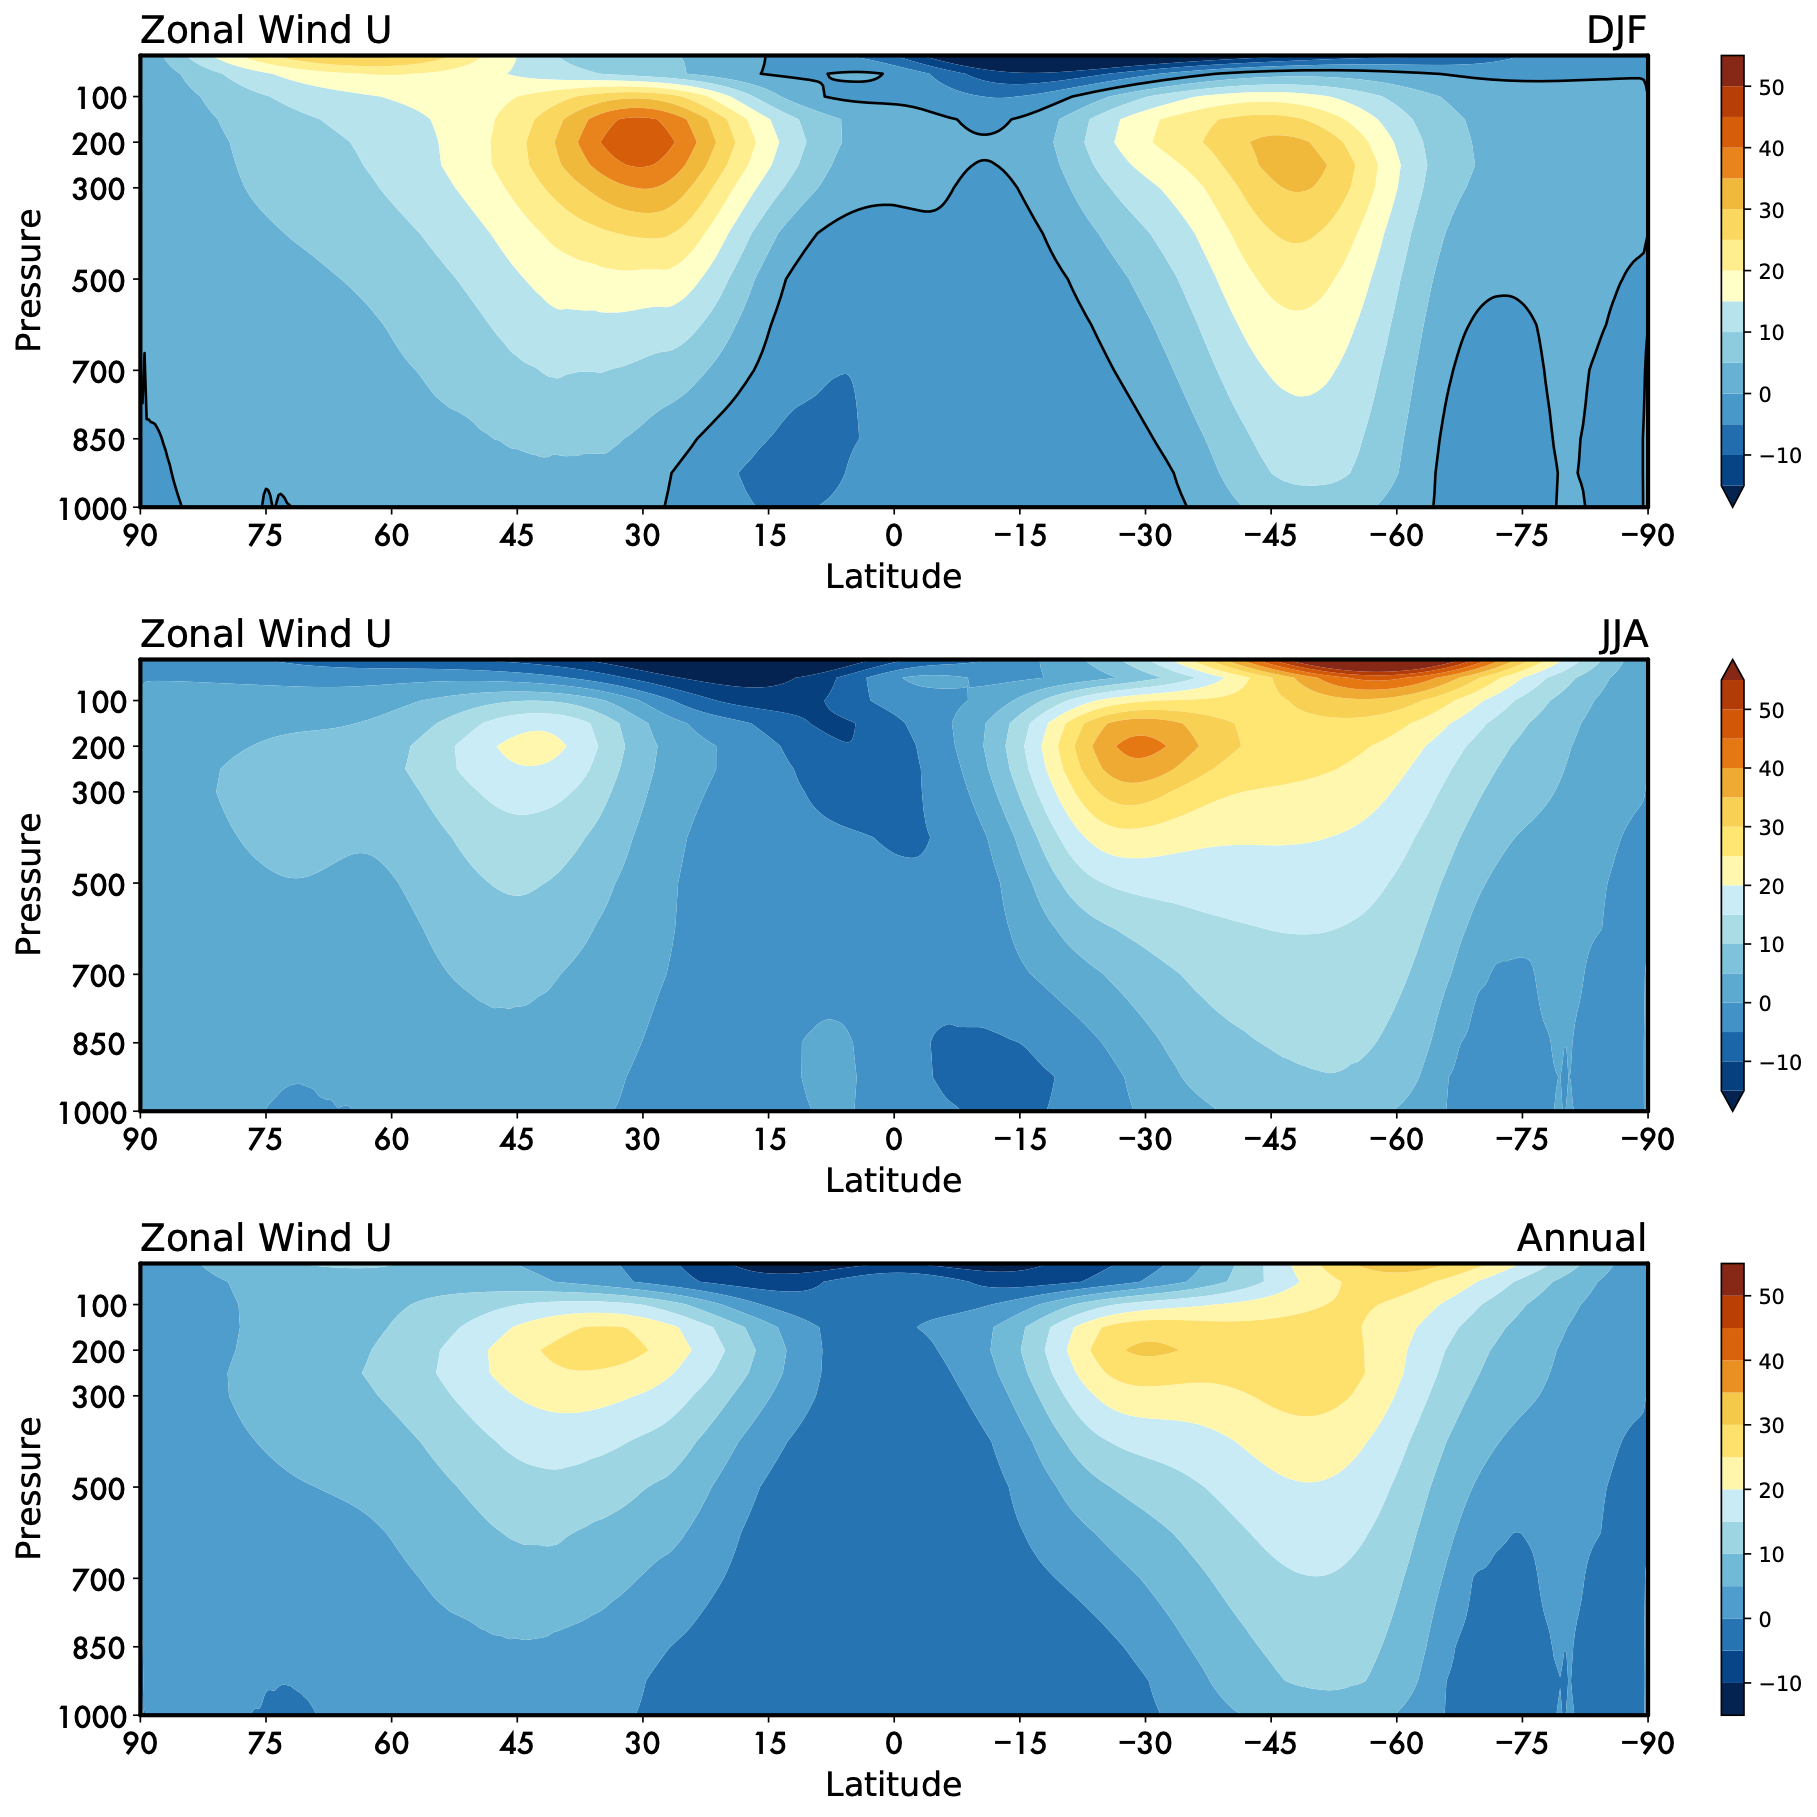
\includegraphics[width = .7 \textwidth]{figs/GD/Uzonal.png}
\caption{}\label{}
\end{figure}

The zonally averaged meridional circulation is shown in
Fig.(\texttt{fig:52}). It is possible to see the low level convergence
at the equator and high level divergence of the flow. The annual mean
show more clearly the direct circulation that is located between the
tropics. Note that the point of convergence, the InterTropical
Convergence Zone  ITCZ, though is generally following the seasonal
cycle of the sun is asymmetric with respect the equator, oscillating
between \(15N\) and \(5S\).

\begin{figure}
\centering
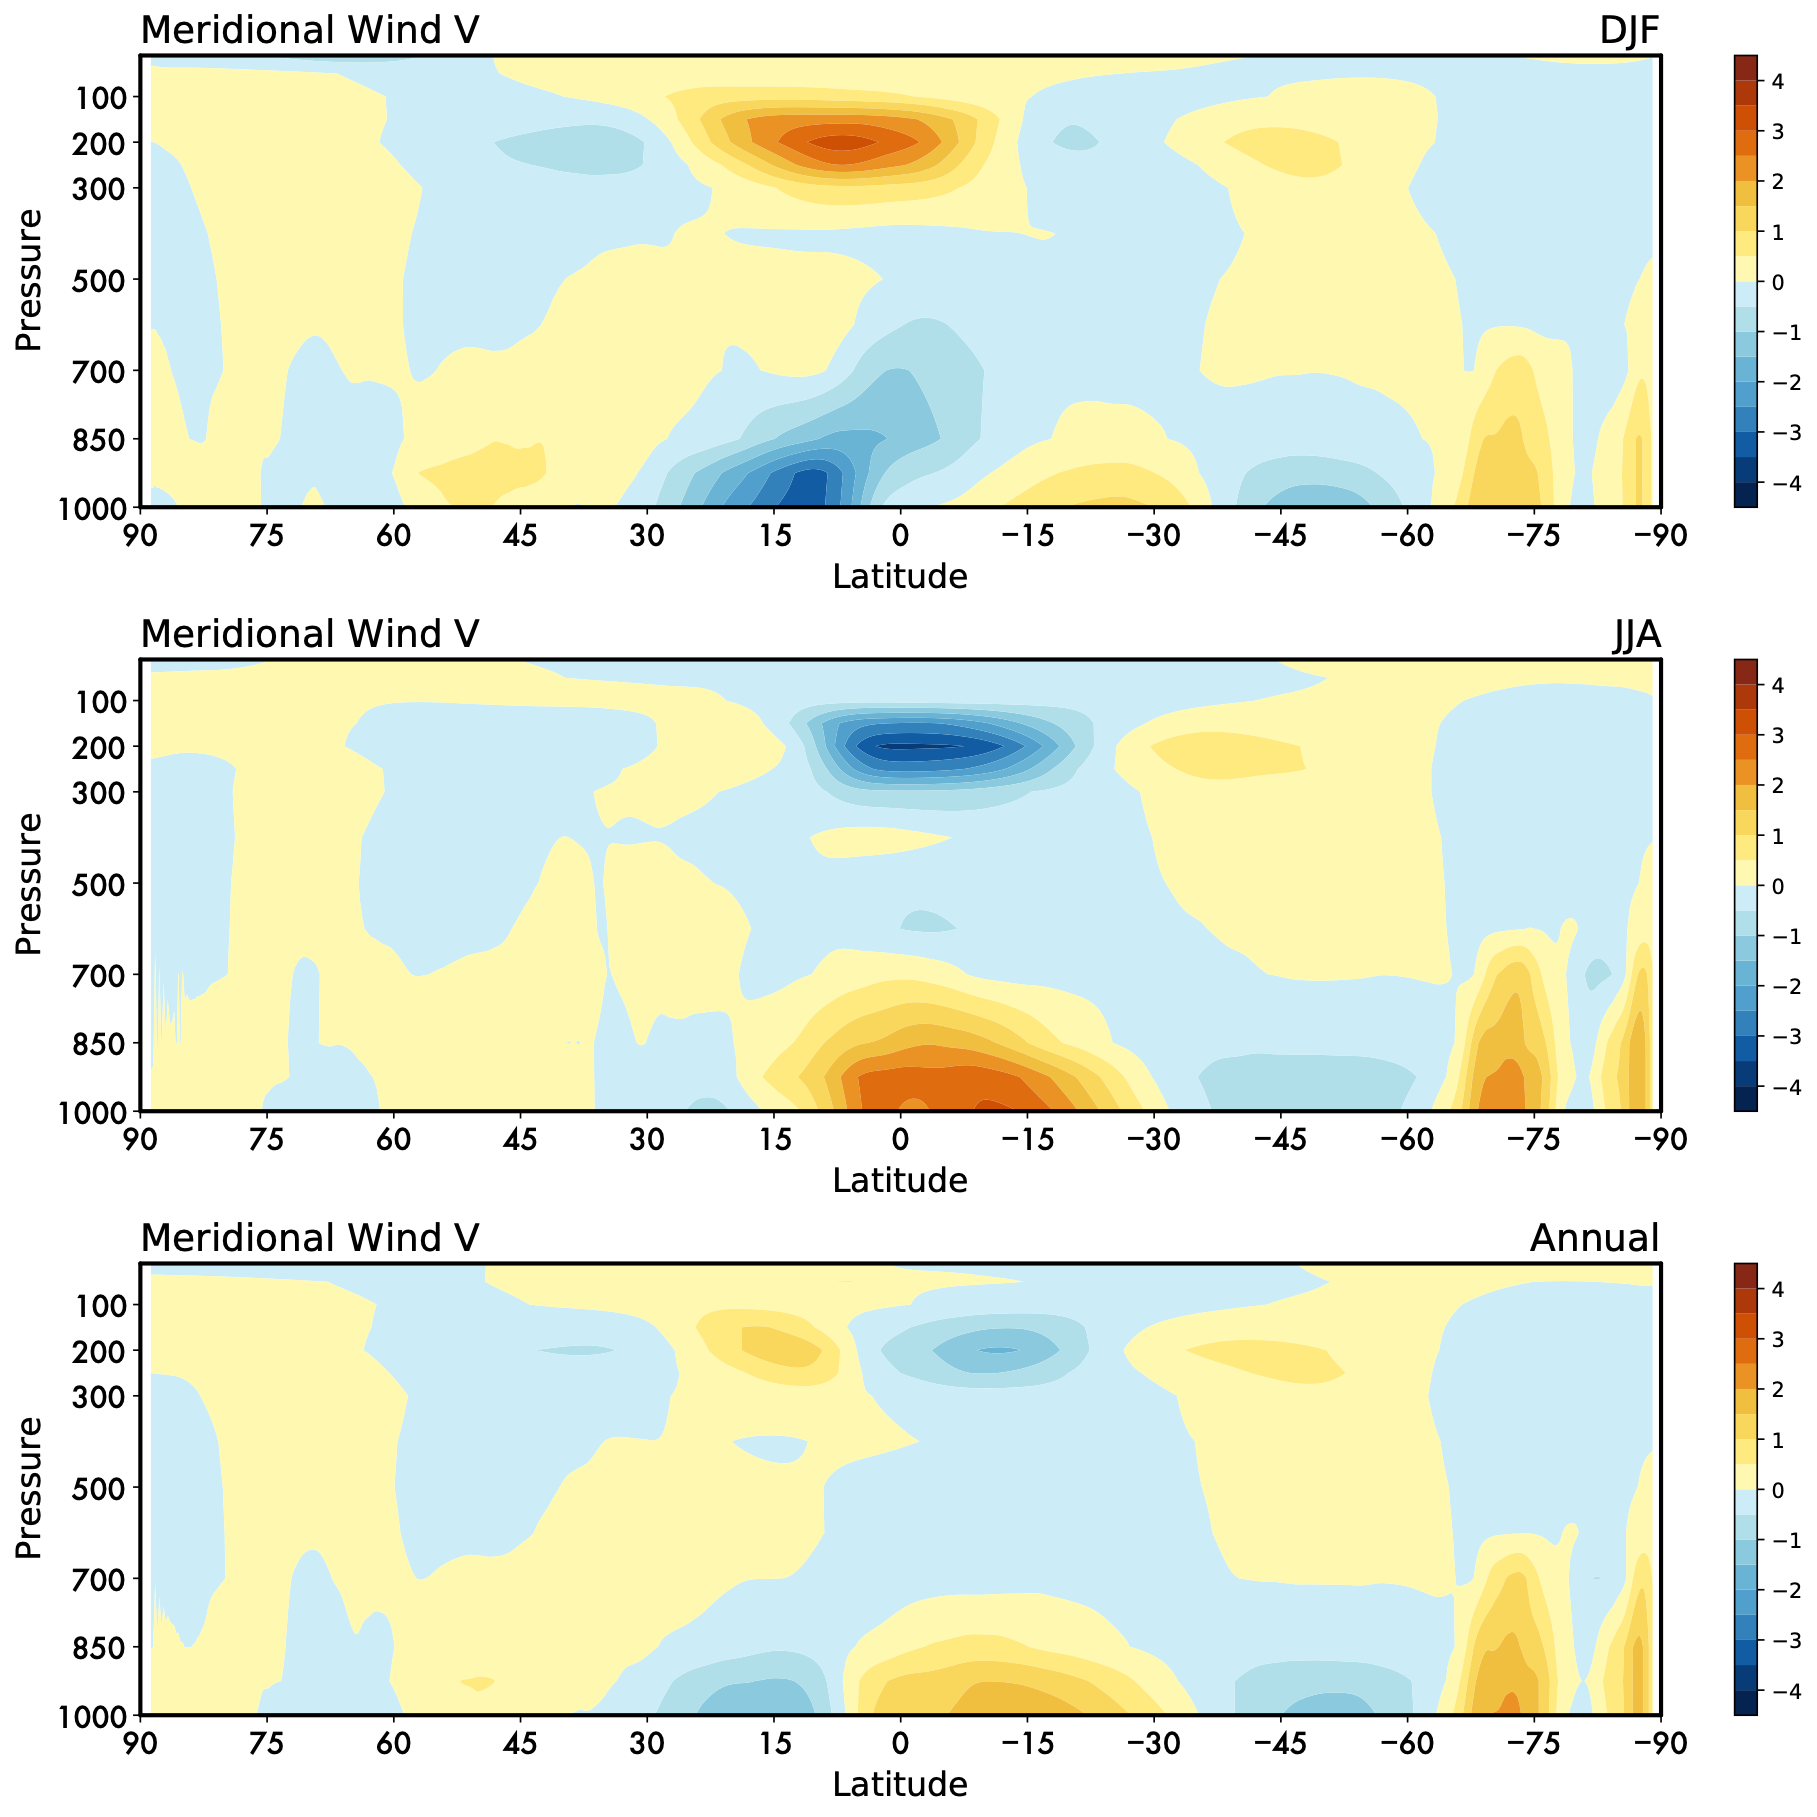
\includegraphics[width = .7 \textwidth]{figs/GD/Vzonal.png}
\caption{}\label{}
\end{figure}

The thermal structure is shown in Fig. \texttt{fig:53}. As a consequence
of the radiation balance the temperature is decreasing with latitude.
The equatorial area is receiving excess radiation with respect to the
the polar region. The hydrostatic balance is shown in the decreasing
temperature with height, but the lapse rate is less than adiabatic,
indicating the average stable nature of the atmosphere. There is a
strong latitudinal gradient in temperature, but the gradient is
decreasing with altitude and is actually reversing sign in the upper
atmosphere and stratosphere.

This is caused by the radiation absorption by ozone and other components
in the lower stratosphere. The change of sign of the temperature
meridional gradient Fig. \texttt{fig:531} is also consistent with the
structure of the zonal wind, with positive shear in the troposphere and
negative shear above it, consistent with the thermal wind balance.

\begin{figure}
\centering
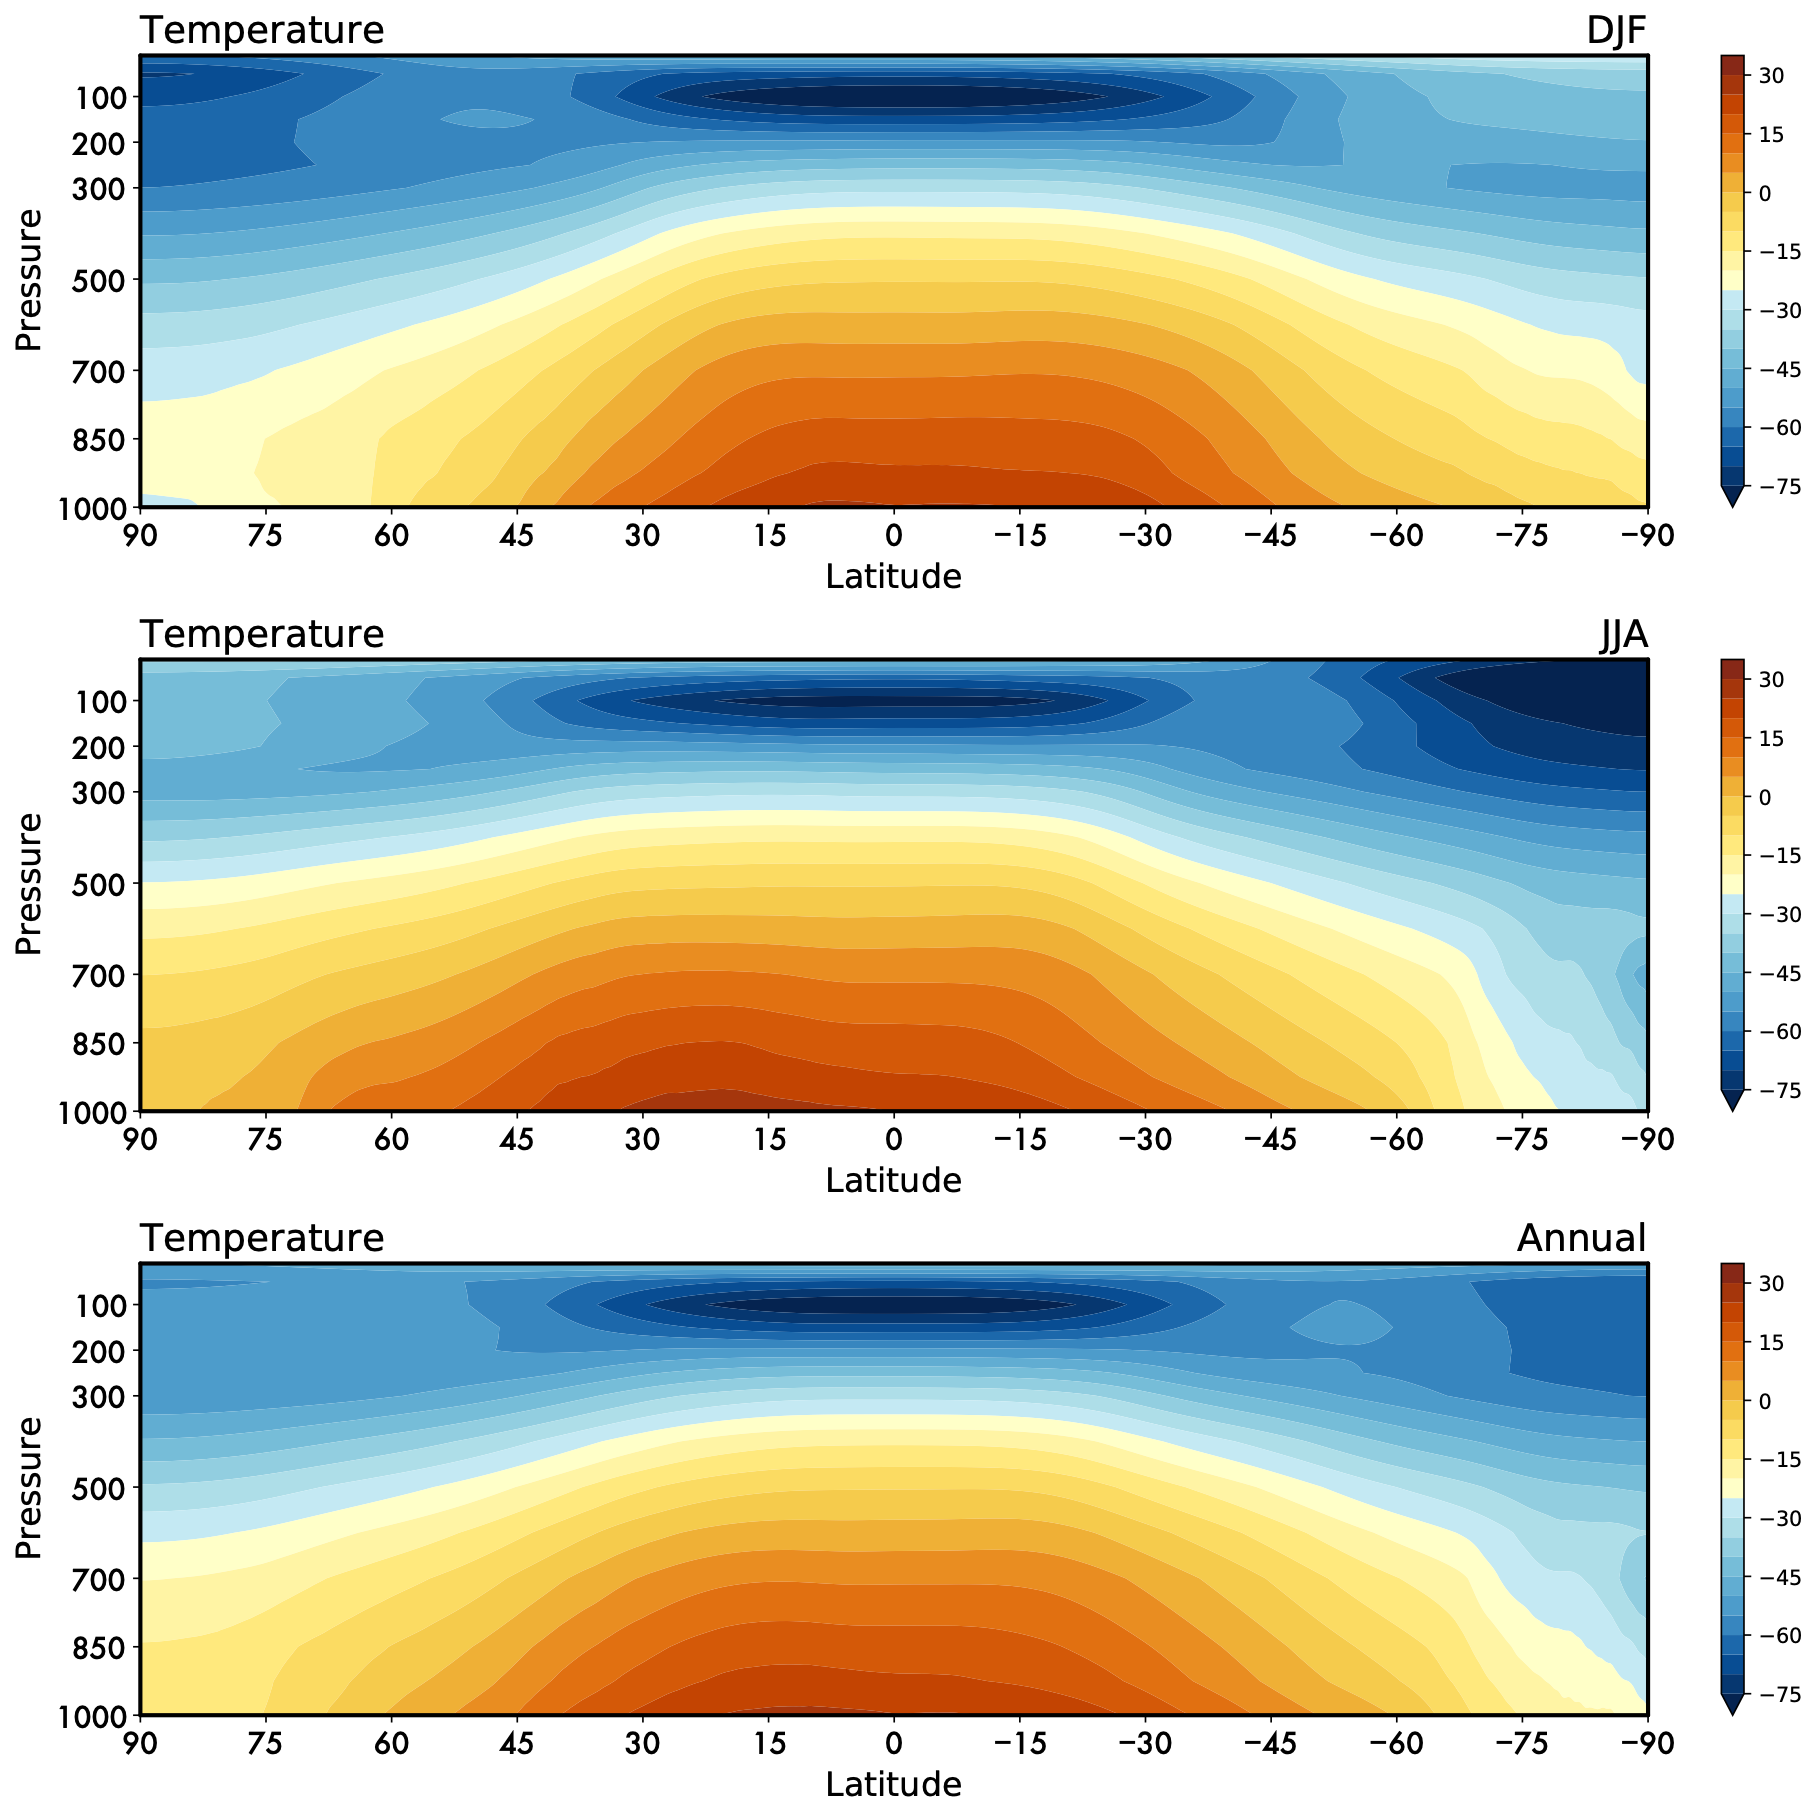
\includegraphics[width = .7 \textwidth]{figs/GD/Tzonal.png}
\caption{}\label{}
\end{figure}

\begin{figure}
\centering
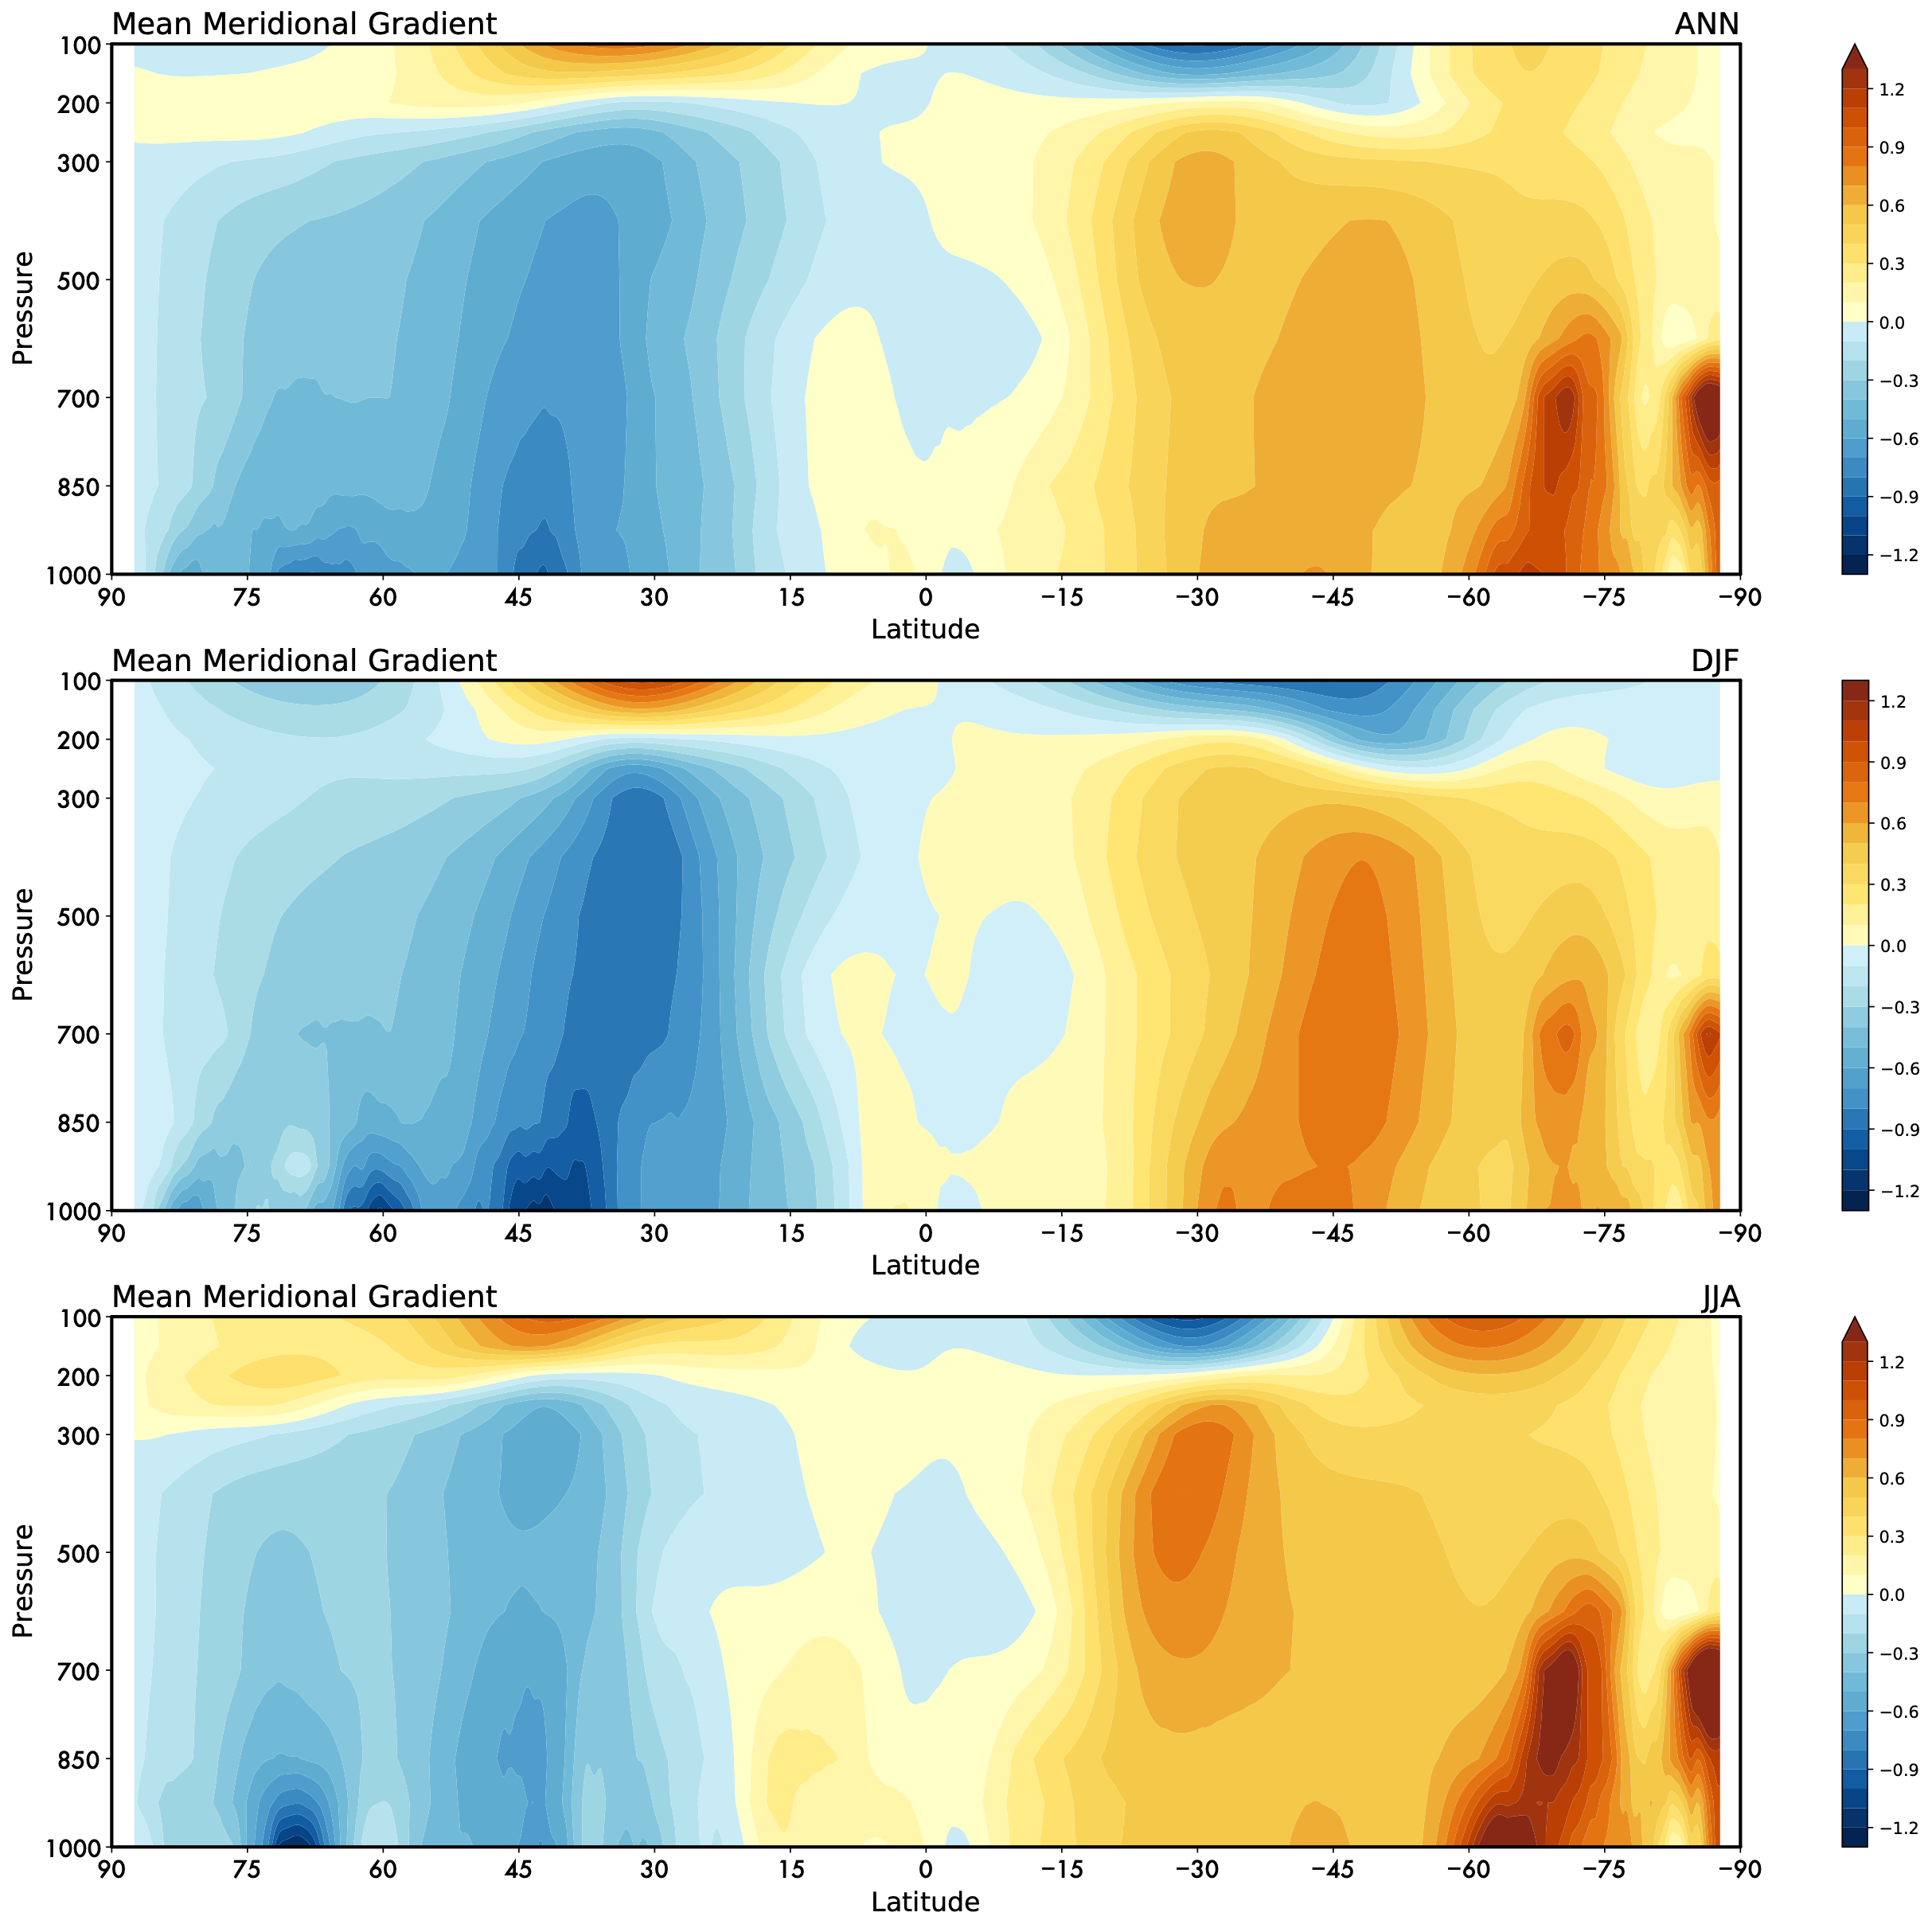
\includegraphics[width = .7 \textwidth]{figs/GD/Tgradient.png}
\caption{}\label{}
\end{figure}

The structure of the distribution of water vapor in the atmosphere is
shown in Fig. \texttt{fig:532}. The water vapor is shown as the
\emph{specific humidity} that is mass of water vapour in a unit mass of
moist air, usually expressed as grams of vapour per kilogram of air. The
annual average (bottom) shows how the water vapor is strongly confined
to the lower levels and to the equatorial zone. The atmosphere is very
dry as the altitude increases. This is a direct consequence of the
strong dependence on temperature of the Clausius-Clayperon equation that
describes how the saturation water vapor pressure changes with
temperature. At the equator, really moist air contains 12-15 grams of
water per kilogram of moist air.

The seasonal distributions (other panels in Fig. \texttt{fig:532}) show
a shift of specific humidity in latitude roughly following the seasonal
cycle of the sun. The surface maximum is located around 5S in DJF and
then shifts to around 10N in JJA. The Winter hemisphere in both seasons
is definitely more moist at the surface than the Summer, but values are
smaller than the equatorial zone, reaching at most around 8 g/kg.

\begin{figure}
\centering
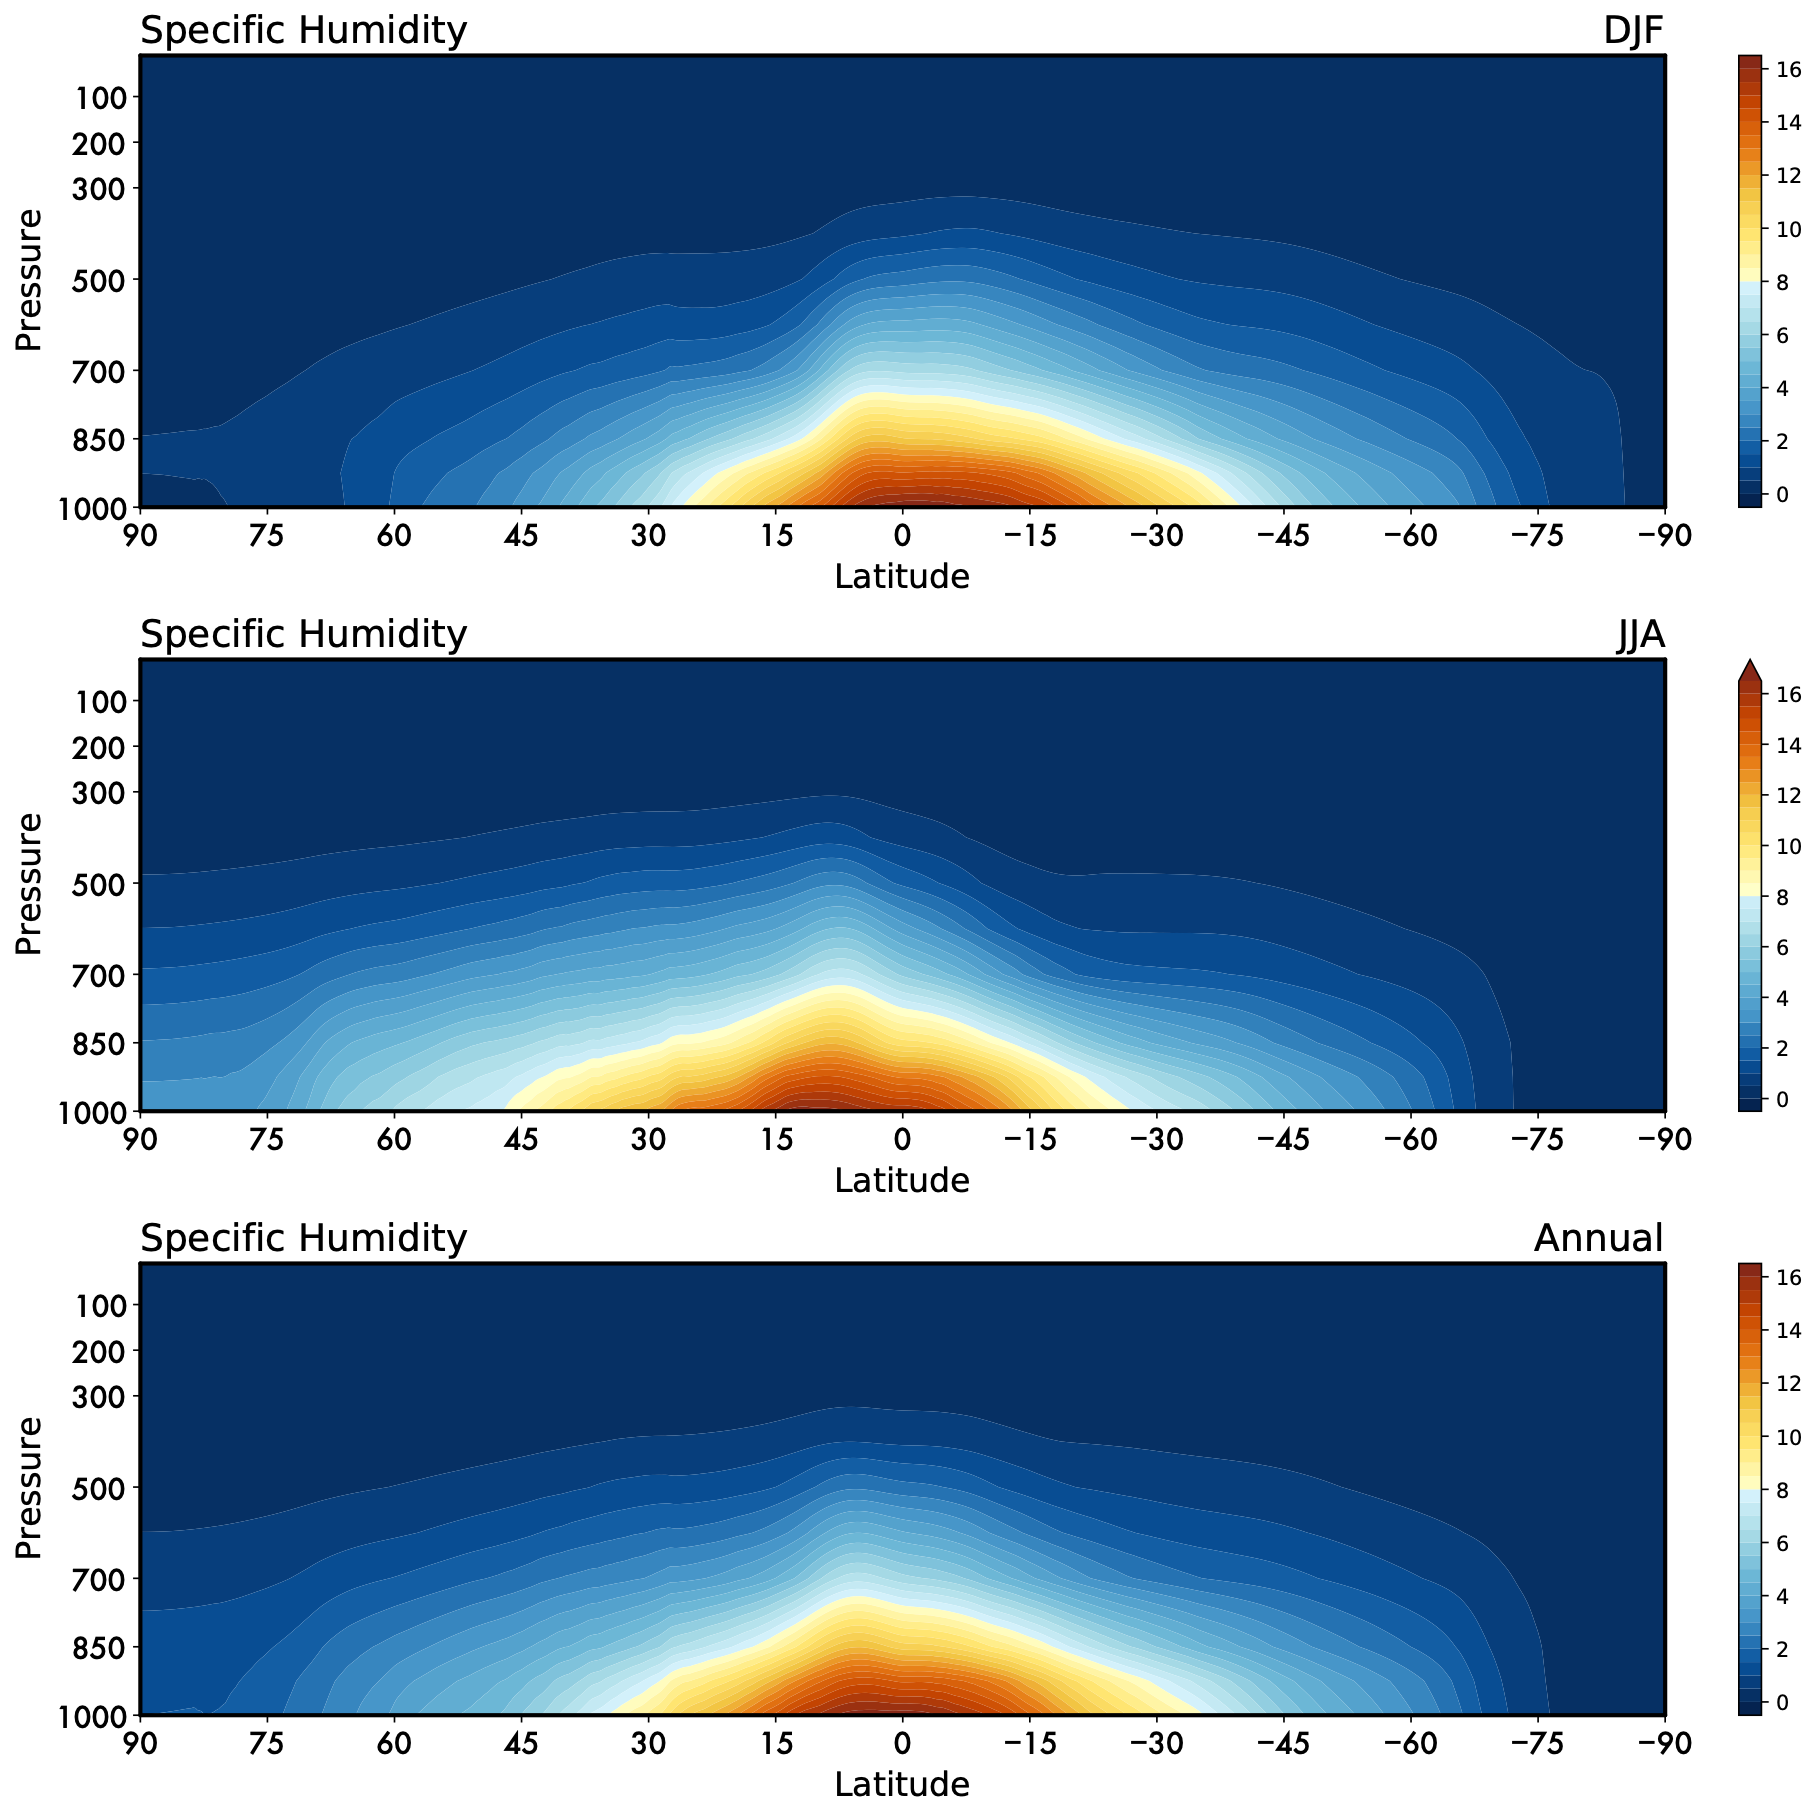
\includegraphics[width = .7 \textwidth]{figs/GD/Qzonal.png}
\caption{}\label{}
\end{figure}

. {[}fig:532{]}

\begin{figure}
\centering
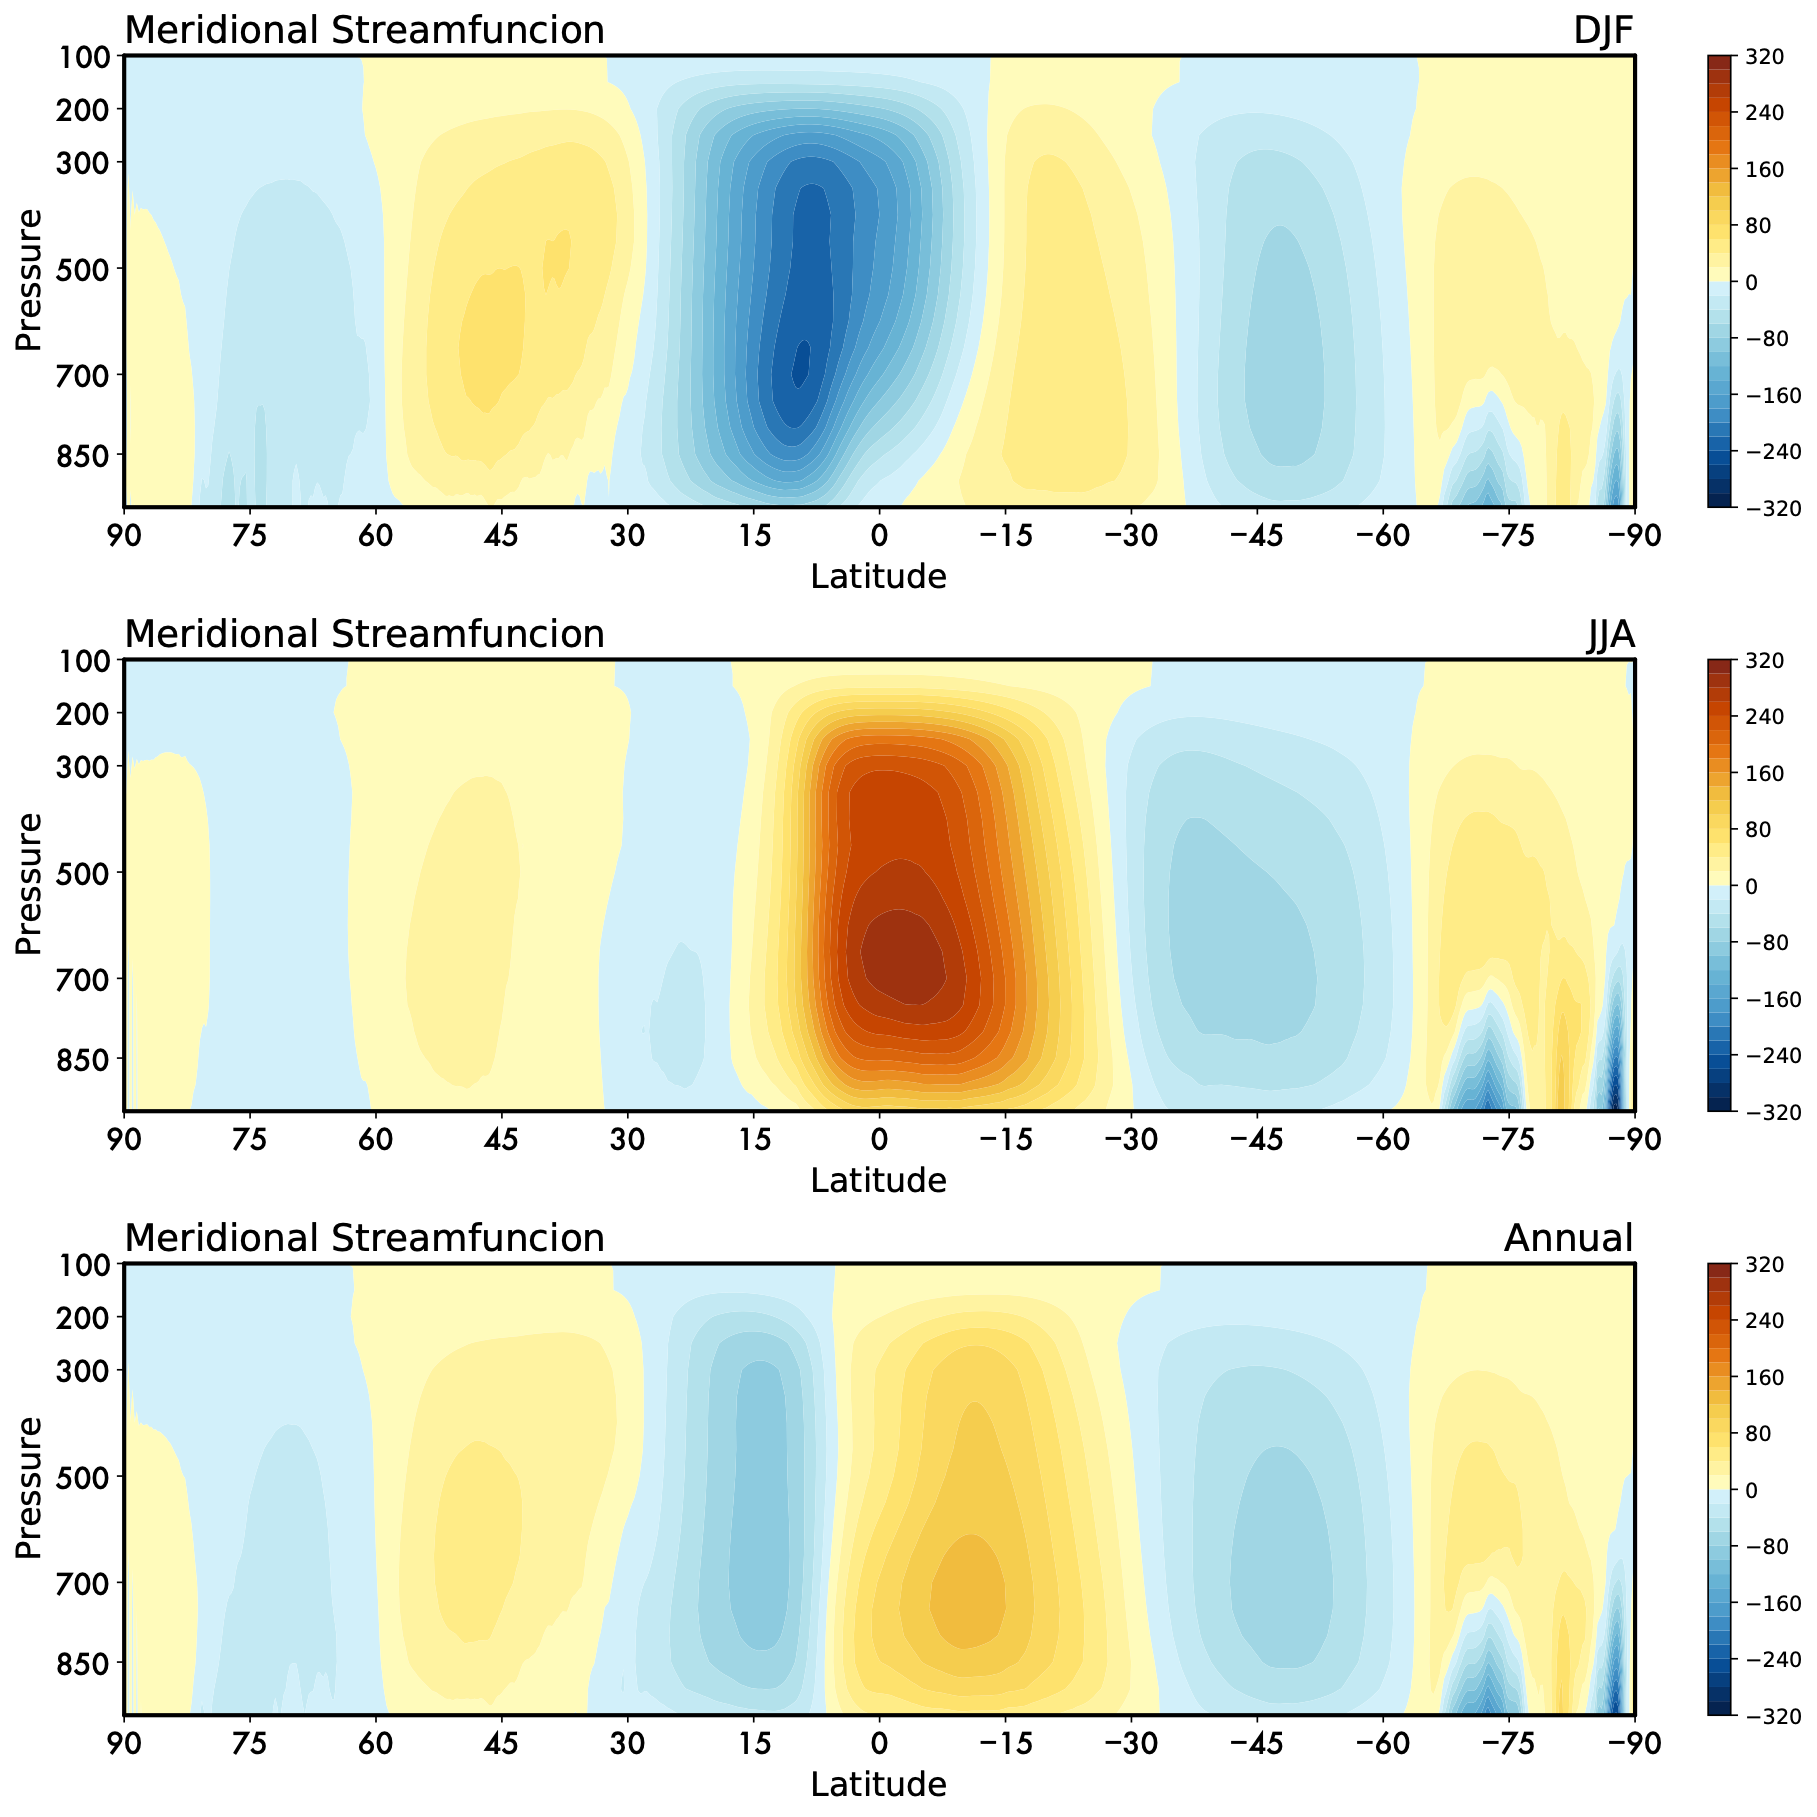
\includegraphics[width = .7 \textwidth]{figs/GD/MSzonal.png}
\caption{}\label{}
\end{figure}

\subsection{The horizontal general
circulation}\label{the-horizontal-general-circulation}

Fig. \texttt{fig:551} shows the climatological geopotential height for
DJF at 200mb. The top panel shows the full field. The geostrophic
balance implies that it can be considered as an approximate
streamfunction for the horizontal flow. The bottom panel shows the same
field with the zonal mean removed, the eddy component. It shows clearly
the large deviations from the zonally symmetric circulation located over
the east coast of continents. A more careful inspection may reveal that
they are downstream from large continental size mountain ranges, the
Rocky Mountains and the Himalayan Plateau.

\begin{figure}
\centering
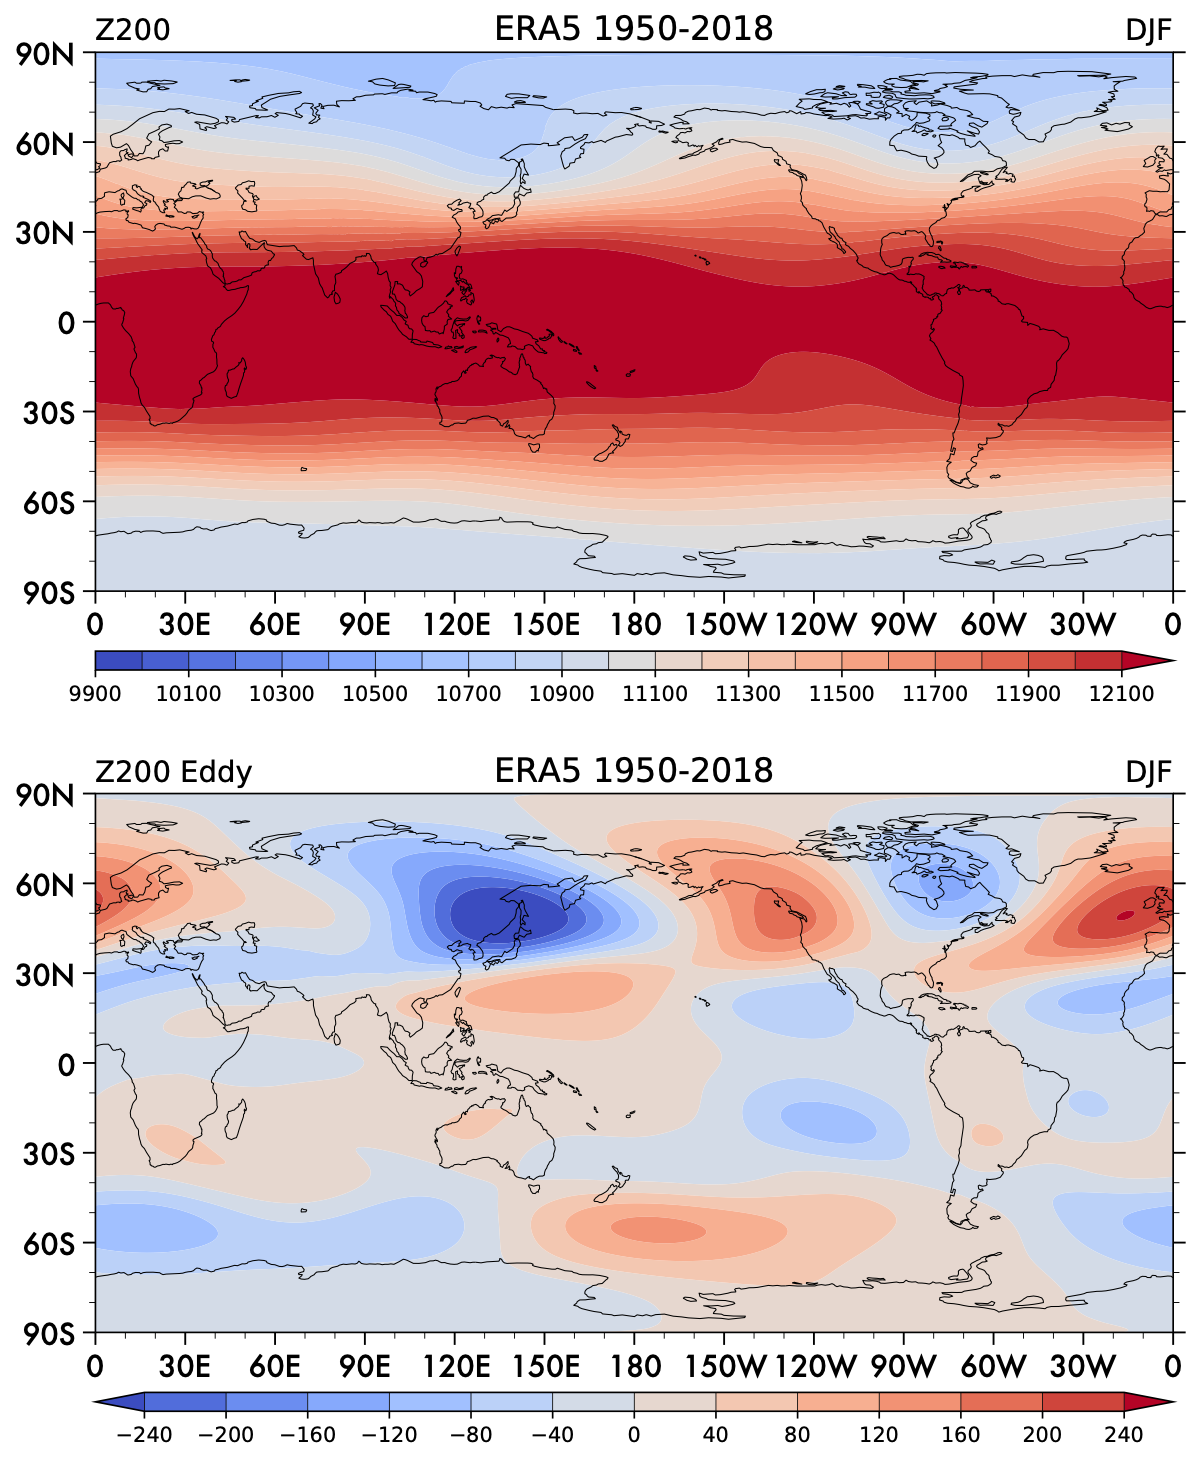
\includegraphics[width = .7 \textwidth]{figs/GD/Z200.png}
\caption{}\label{}
\end{figure}

A better insight is provided by using a special polar projection to
inspect the Geopotential field. There are several geographical
projection to represent quantity on the sphere on a map and each of them
is useful to enhance some property of the flow. The shape of the
hemispheric circumpolar vortex is for instance clearly represented in
the stereo projection of Fig. \texttt{fig:552}. it is possbile to see
the curvature of the flow downstream of the Rocky Mountains and the
Himalayas and the typical shape of the Winter climatological pattern of
the high altitude atmospheric geopotential.

\begin{figure}
\centering
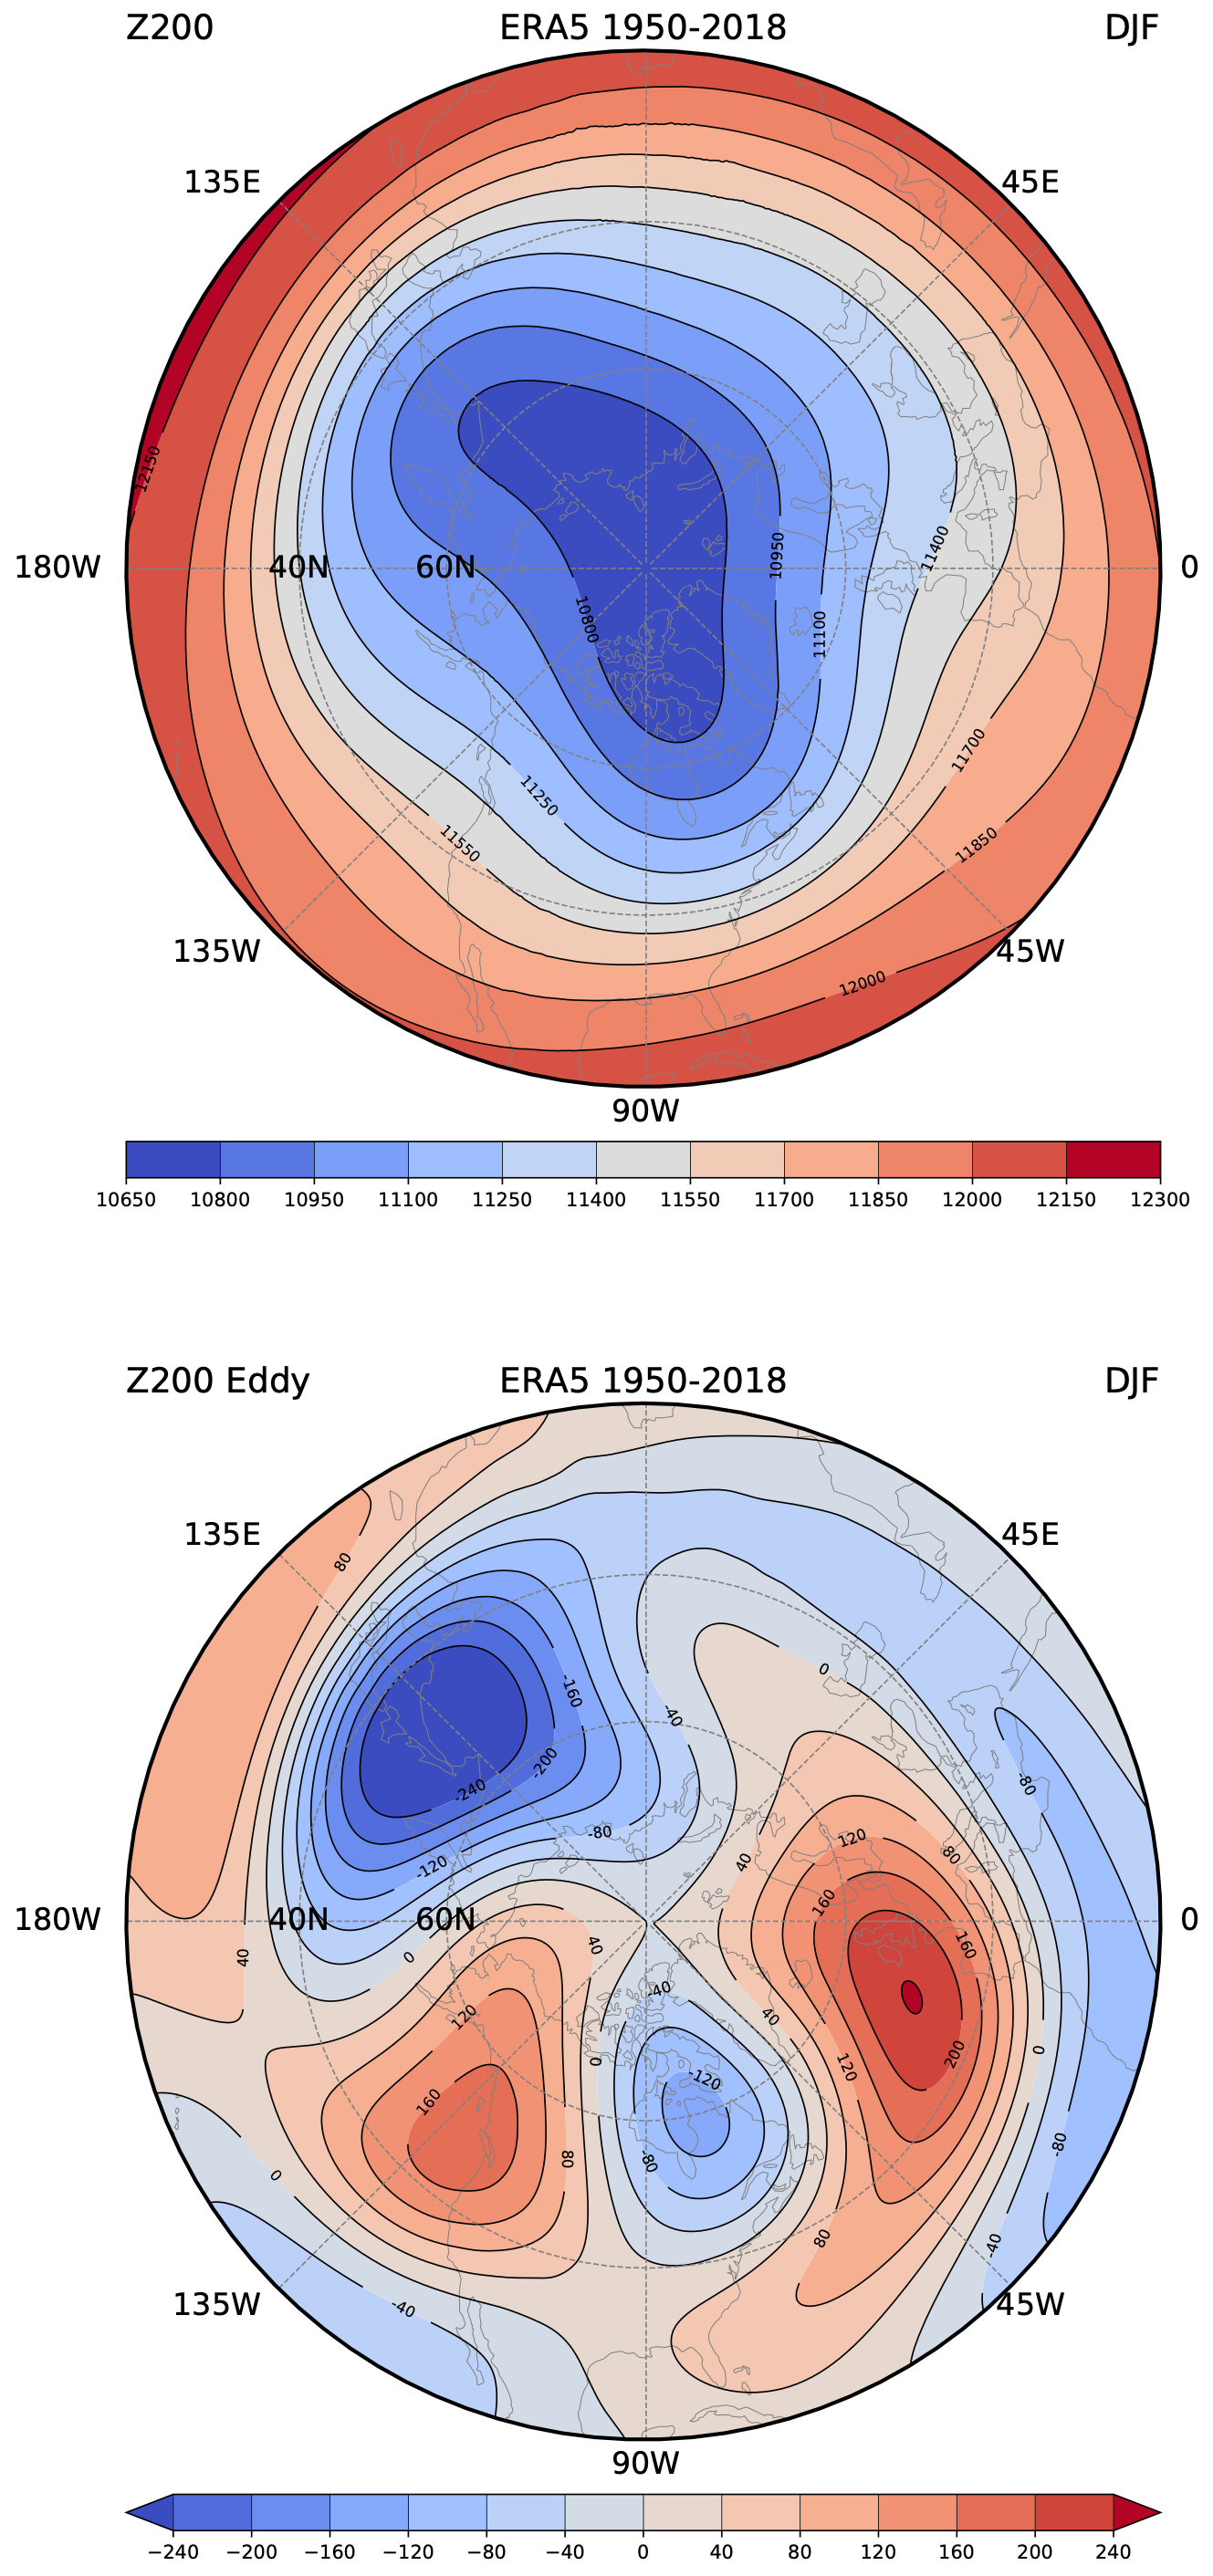
\includegraphics[width = .7 \textwidth]{figs/GD/Z200NH.png}
\caption{}\label{}
\end{figure}

\subsubsection{The horizontal wind}\label{the-horizontal-wind}

The geopotential is a good approximation to the streamfunction in the
mid-latitudes where the geostrophic balance controls tightly the
dynamical balance, but it gives usa poor ideas of the wind circulation
in the low latitudes. In this case is better to look at the wind
directly. Fig. \texttt{fig:56} shows the zonal wind at 200mb for the
calendar Winter (DJF) and Summer (JJA). We can see clearly the westerly
jet streams in the winter of both hemispheres. The jets are concentrated
on the east coast of both large continental land masses.

The Asian jet is the most intense, reaching at its core a velocity in
excess of 70 m/s. In comparison, the North American jet is weaker and
smaller in longitudinal extent. The winter jet in the Southern
Hemisphere is also well formed, but at this level is not at the same
amplitude of the northern hemisphere jets. Summer westerly jets are also
present in both summer hemisphere, but much weaker.

The tropical region instead is characterised by easterly jets, most
prominent over the maritime continent and the equatorial South America.
In Summer the Easterly circulation over the Indian Ocean is very
intense. The longitudinal gradient of the wind implies areas of
divergent flow over South America and the Indonesian region.

The meridional wind in winter (DJF) (Fig. \texttt{fig:57}) shows the
alternating patterns of positive and negative (poleward and equatorward)
that are consistent with the eddy pattern of the geopotential. Large
deviations from the zonal mean occur over the Pacific-North American
sector and over Far East Asia. In the calendar Summer (JJA) the winds
are weaker and they reach a somewhat large amplitude only over the
southern hemisphere.

Close to the surface (Fig. \texttt{fig:55}) the zonal wind is in general
weaker over land, but stronger over the ocean, and it is clearly
westerly in the mid latitudes, whereas easterlies dominates the
subtropical zone, with the notable exception of the Indonesian Region,
also called the Maritime Continent, where is westerly. The combination
of Easterlies and Westerlies in the equatorial Pacific point to a near
surface convergence area somewhere in the Central Pacific Ocean.

In JJA the zonal wind shows the seasonal cycle and it gets strength in
the winter hemisphere, retaining the general features that we have seen
for the Winter. Note instead the strong westerlies in the Indian Ocean.
This is the first evidence of the seasonal monsoonal circulation in the
Indian subcontinent. The Easterlies south of the westerlies indicates a
possible circulation over the Indian Ocean basin.

\begin{figure}
\centering
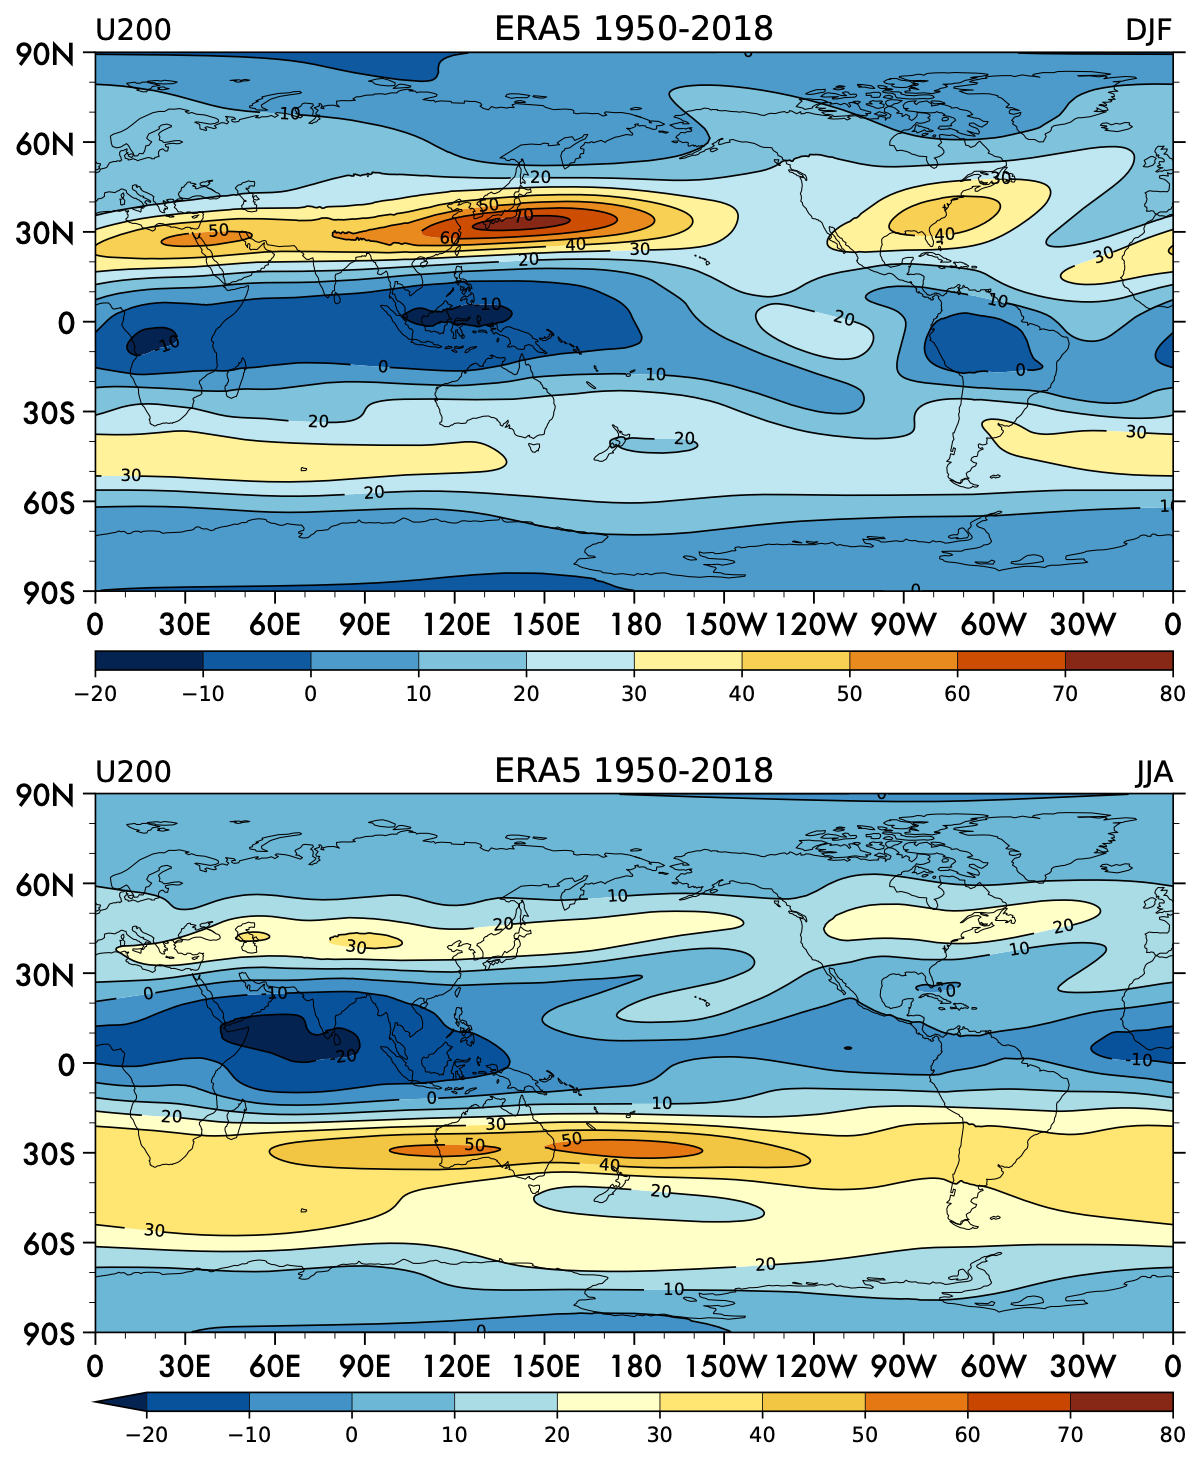
\includegraphics[width = .7 \textwidth]{figs/GD/U200.png}
\caption{}\label{}
\end{figure}

\begin{figure}
\centering
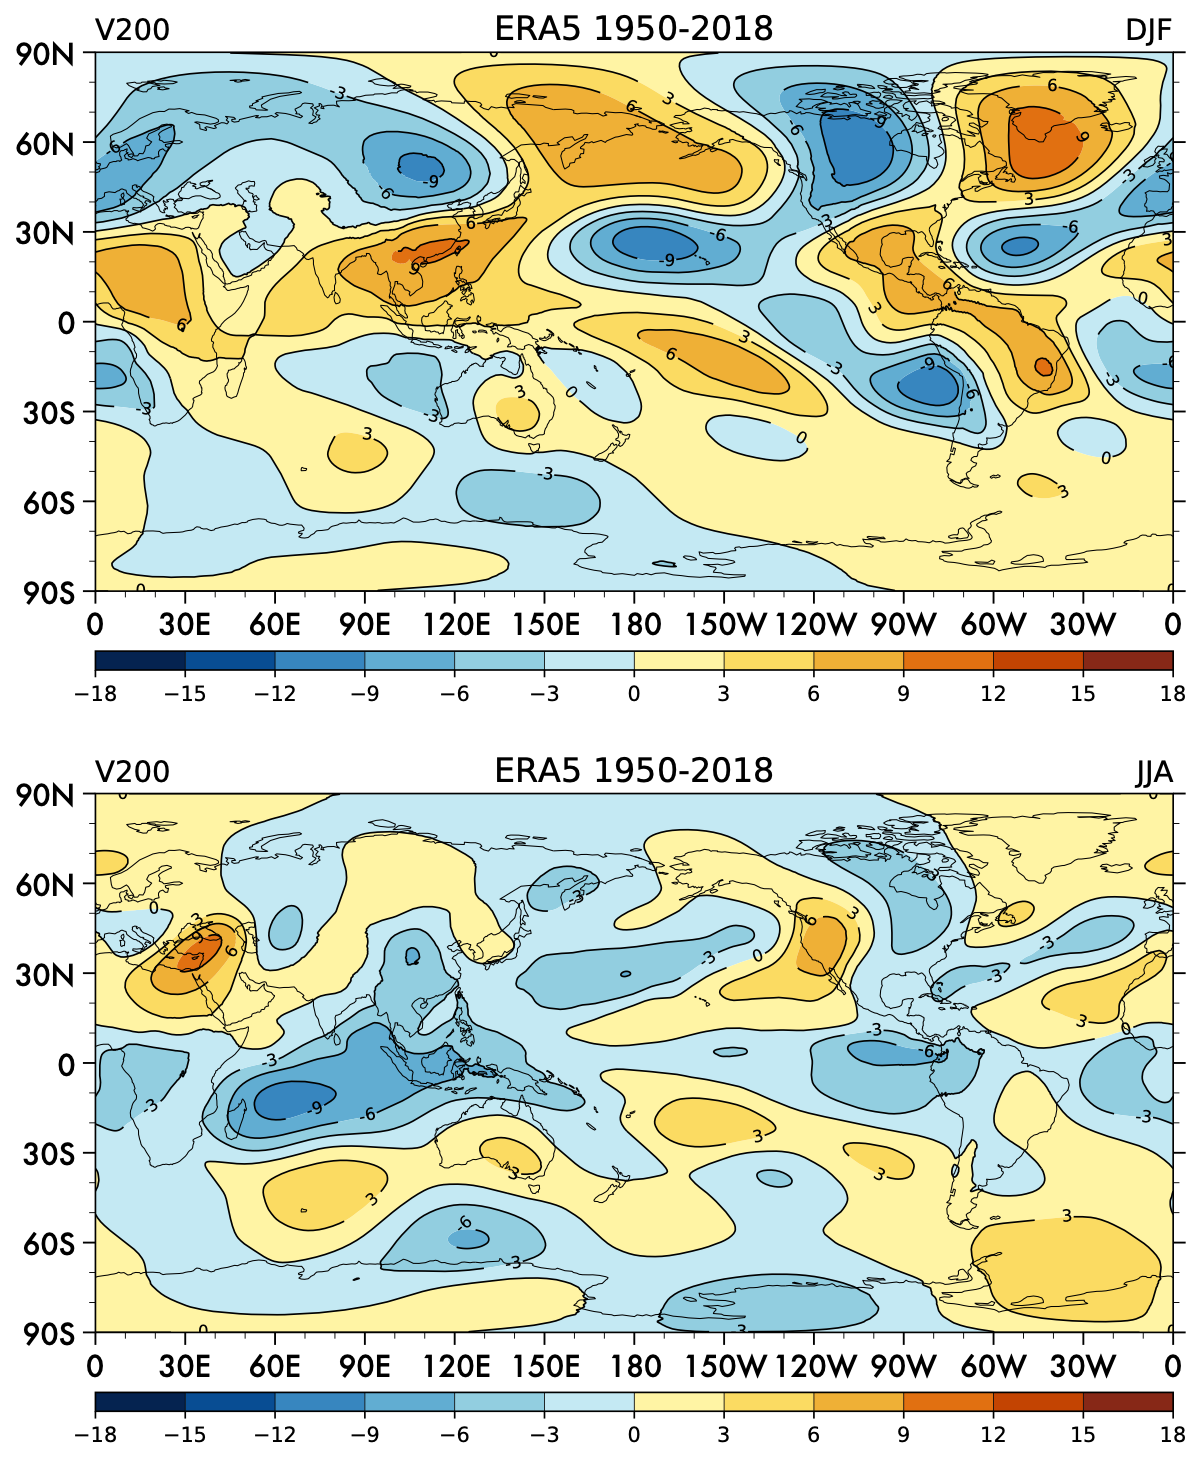
\includegraphics[width = .7 \textwidth]{figs/GD/V200.png}
\caption{}\label{}
\end{figure}

The meridional wind near the surface (Fig. \texttt{fig:58}) shows
dramatic features. Neglecting the areas of high elevation (the Himalaya
plateau, Antarctica) where this pressure level is under ground and
therefore not particularly meaningful, we notice a systematic
equatorward flow over the east coast of continents. It is most intense
along South America, South Africa and the West African coast right North
of the Equator.

In Summer these along shore winds becomes more intense along the North
American and African coast. Interestingly, the flow is reverse along thr
Somali coast in the Indian Ocean. The meridional flow is reversed with
respect the Winter season. In the Summer it is easy to see that this
flow is closing the circle with the zonal flow in Fig. \texttt{fig:55}
creating a cyclonic circulation that is the distinctive tract of the
South Asian Monsoon.

\begin{figure}
\centering
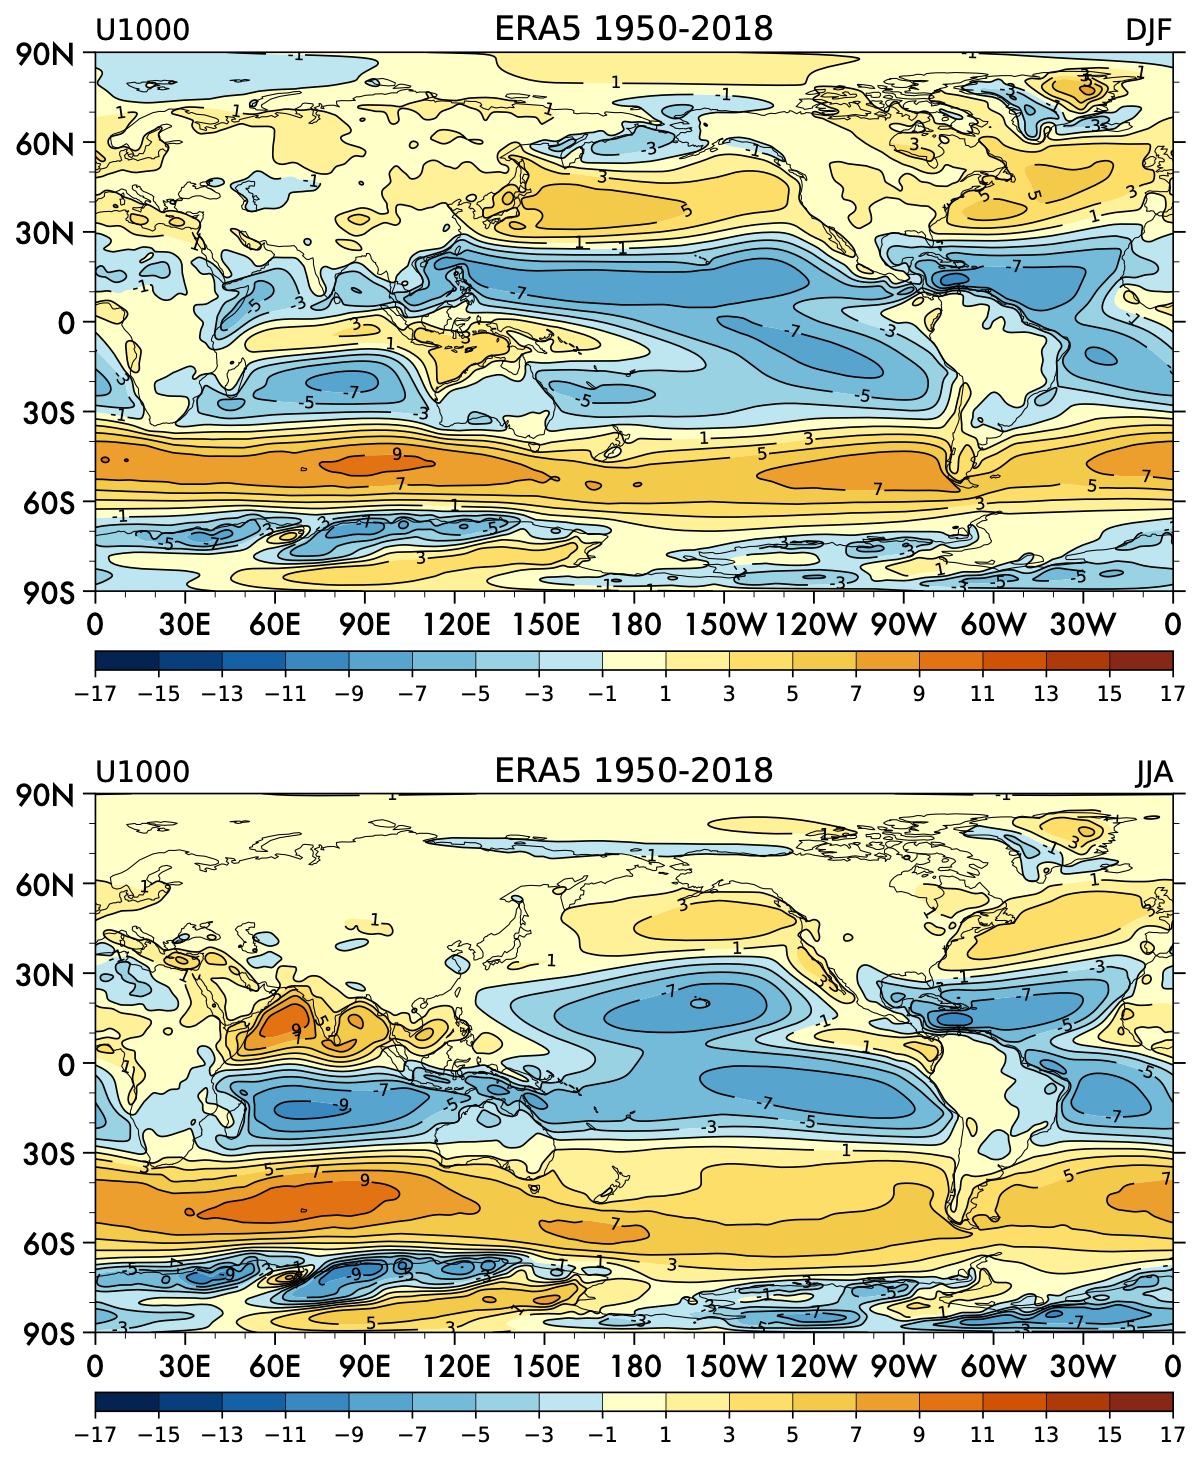
\includegraphics[width = .7 \textwidth]{figs/GD/U1000.png}
\caption{}\label{}
\end{figure}

\begin{figure}
\centering
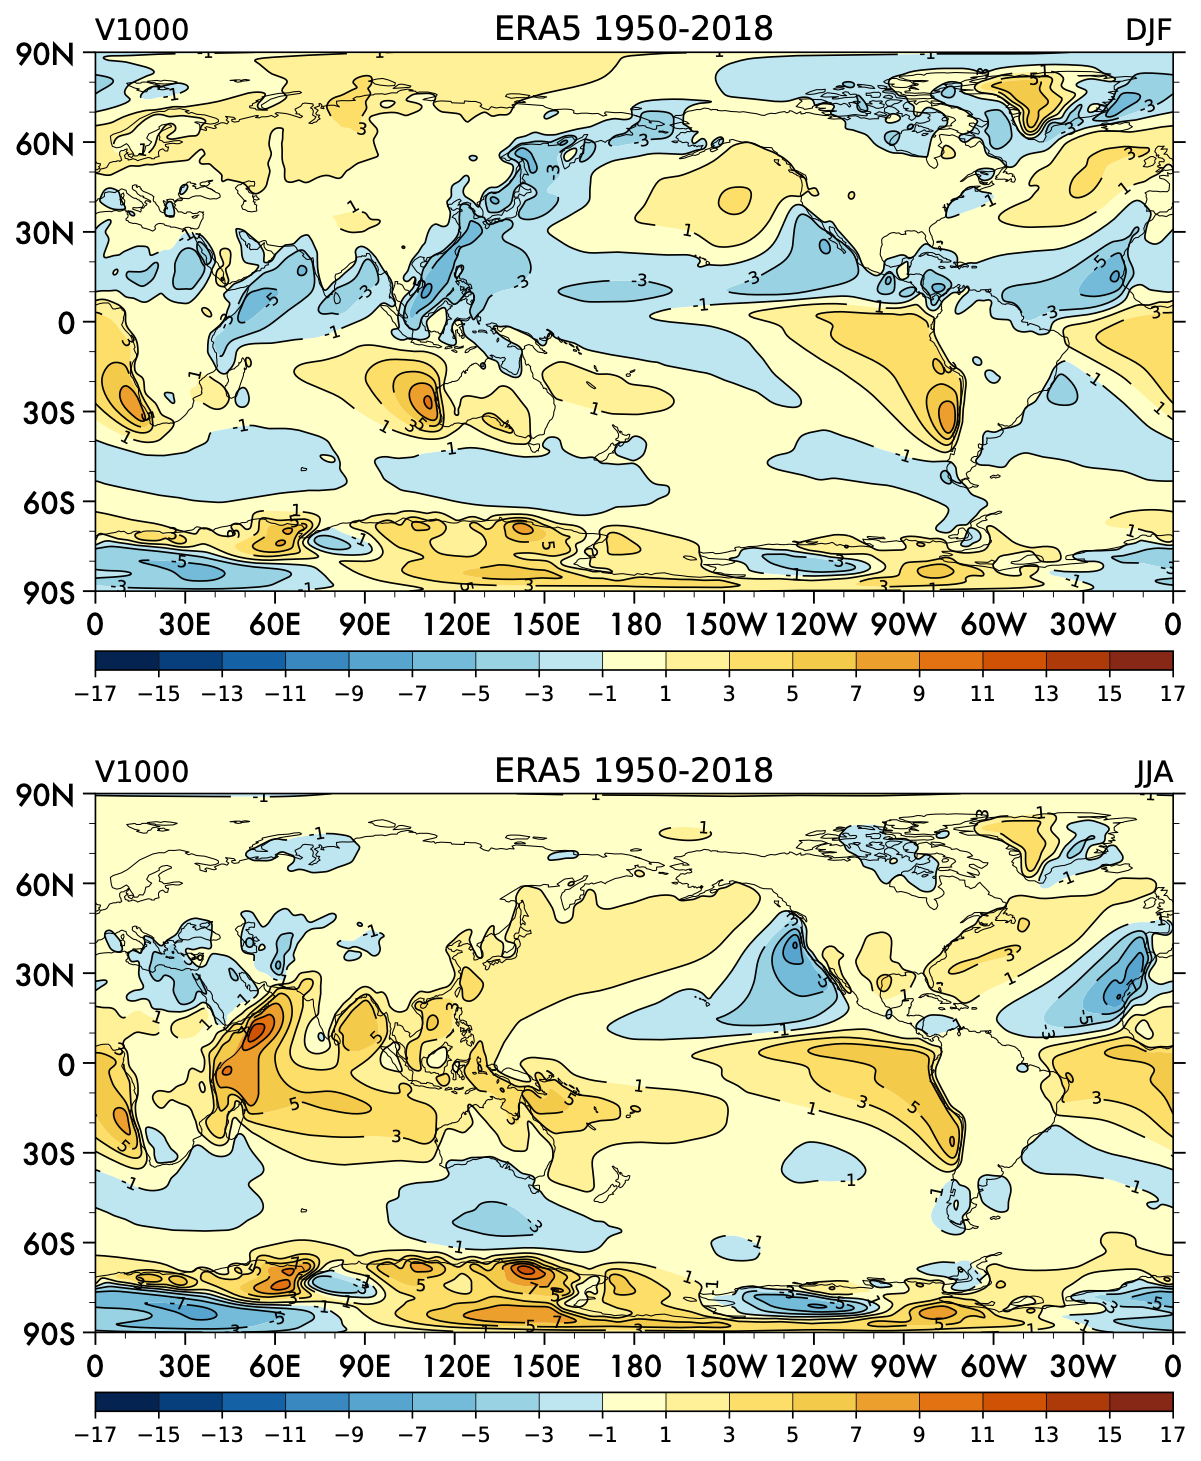
\includegraphics[width = .7 \textwidth]{figs/GD/V1000.png}
\caption{}\label{}
\end{figure}

The \(1000mb\) circulation is very close to the ground and it represent
very well the forcing that the oceans feel from the atmosphere. As such
it is a crucial element of the interactions between atmosphere and
ocean. The real low- level circulation field for the atmosphere is
better represented by a level that is outside of the planetary boundary
layer over most of the planet surface. Such a level is traditionally
considered the \(850mb\) level.

Fig. \texttt{fig:580} shows the streamlines of the wind at 850mb level
in winter and Summer. The equatorial circulation is clearly visible in
the Pacific where the Trade winds cover the equatorial region, shifting
in latitude as they follow the seasonal cycle of the ITCZ. Large gyeres
circulation covers the ocean basin and the Asian Summer Monsoon
circulation in the Indian Ocean is clearly visible, curving from the
East Africa towards the Indian subcontinent and Indochina.

\begin{figure}
\centering
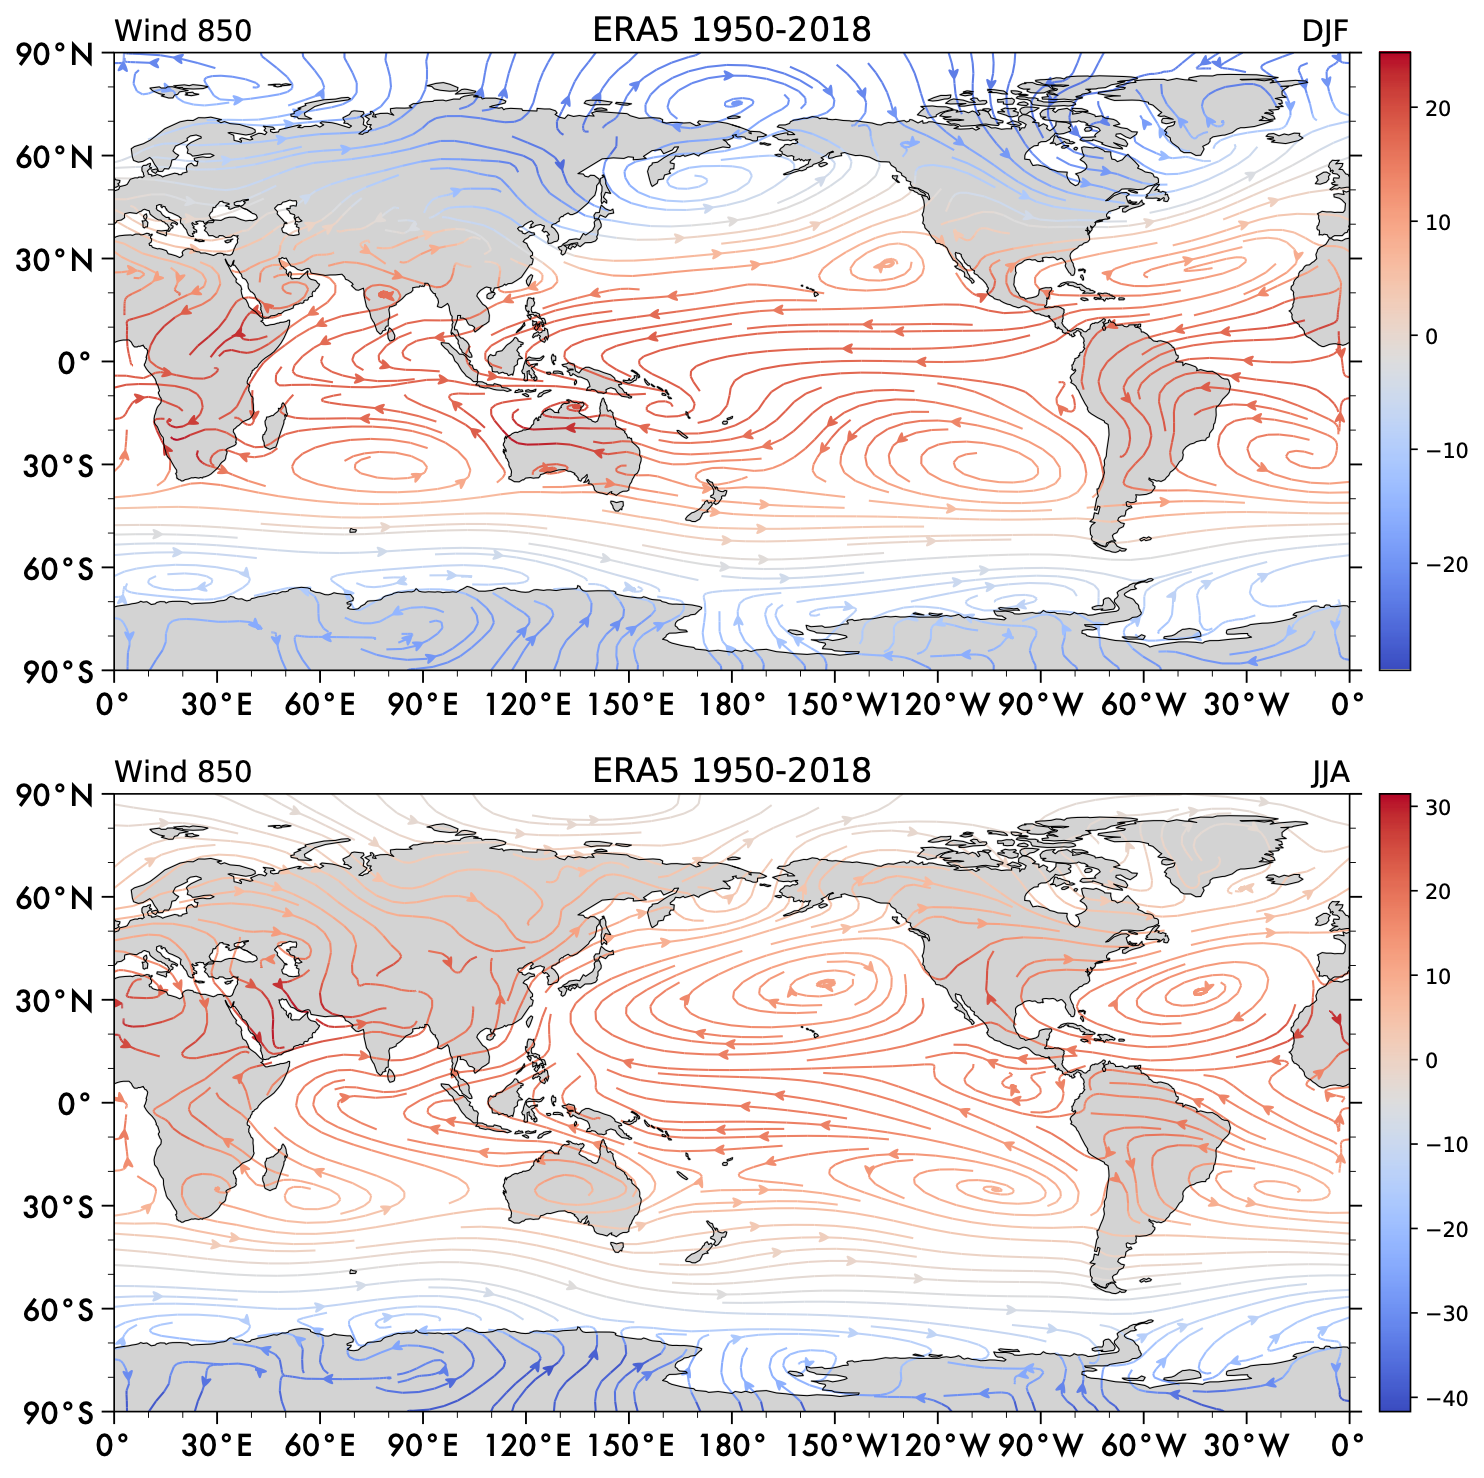
\includegraphics[width = .7 \textwidth]{figs/GD/Wind850.png}
\caption{}\label{}
\end{figure}

\subsubsection{Mean Sea Level Pressure}\label{mean-sea-level-pressure}

The distribution of Mean Sea Level pressure is another important
parameter to describe the general circulation of the atmosphere. This
field is obtained by calculating the pressure at the reference level for
the geopotential (zero level) that is conventionally considered the mean
sea level. It should better referred to as the reference geoid, but most
models still use a spherical Earth approximation, so the zero reference
can still be defined as a sphere.

The principal throwback is that this means that the areas of the Earth
where there are mountains the mean sea level is effectively underground
and therefore of limited usefulness. This especially evident for the
high mountain ranges, the Rockies and the Himalayas and for Antarctica.
Elsewhere, however, it gives a good description of the mass distribution
of the atmosphere. High values of mean sea level pressure correspond to
pile up of mass. The accumulation of mass is larger in the subtropics,
both in Winter and Summer, where a chain of high pressure centers is
present.

The picture is that there are three distinctively different region. The
Northern Hemisphere Midlatitudes, the intertropical region between the
Tropics and the midlatitudes of the Southern Hemisphere. The largest
seasonal contrast emerges in the northern hemisphere mid latitudes. Note
that in Winter high pressure tend to stay over the continent, whereas
low pressure centers develop over the ocean, in Summer it is the
opposite and high pressure stays over the continents.

The Intertropical zone is characterized by the presence of distinct high
pressure centers that oscillate with the season in latitude. The
Southern Hemisphere has a much more symmetric nature with a ring of low
pressure circling the Antarctic continent.

The seasonal cycle is visible in the shift of the ring of high pressure
at the rtropics in the north-south directions. Fig. \texttt{fig:59z}
shows the zonal and time mean for Summer and Winter of the meridional
distribution of sea level pressure. There is a general structure of high
sea level pressure in the tropics, with relative areas of low pressure
in the mid-latitudes and at the Equator. In the Southern hemisphere it
is ismuch more pronounced andf the gradients are much stronger. The
seasonal shift can be seen in the movement of tropical maxima.

\begin{figure}
\centering
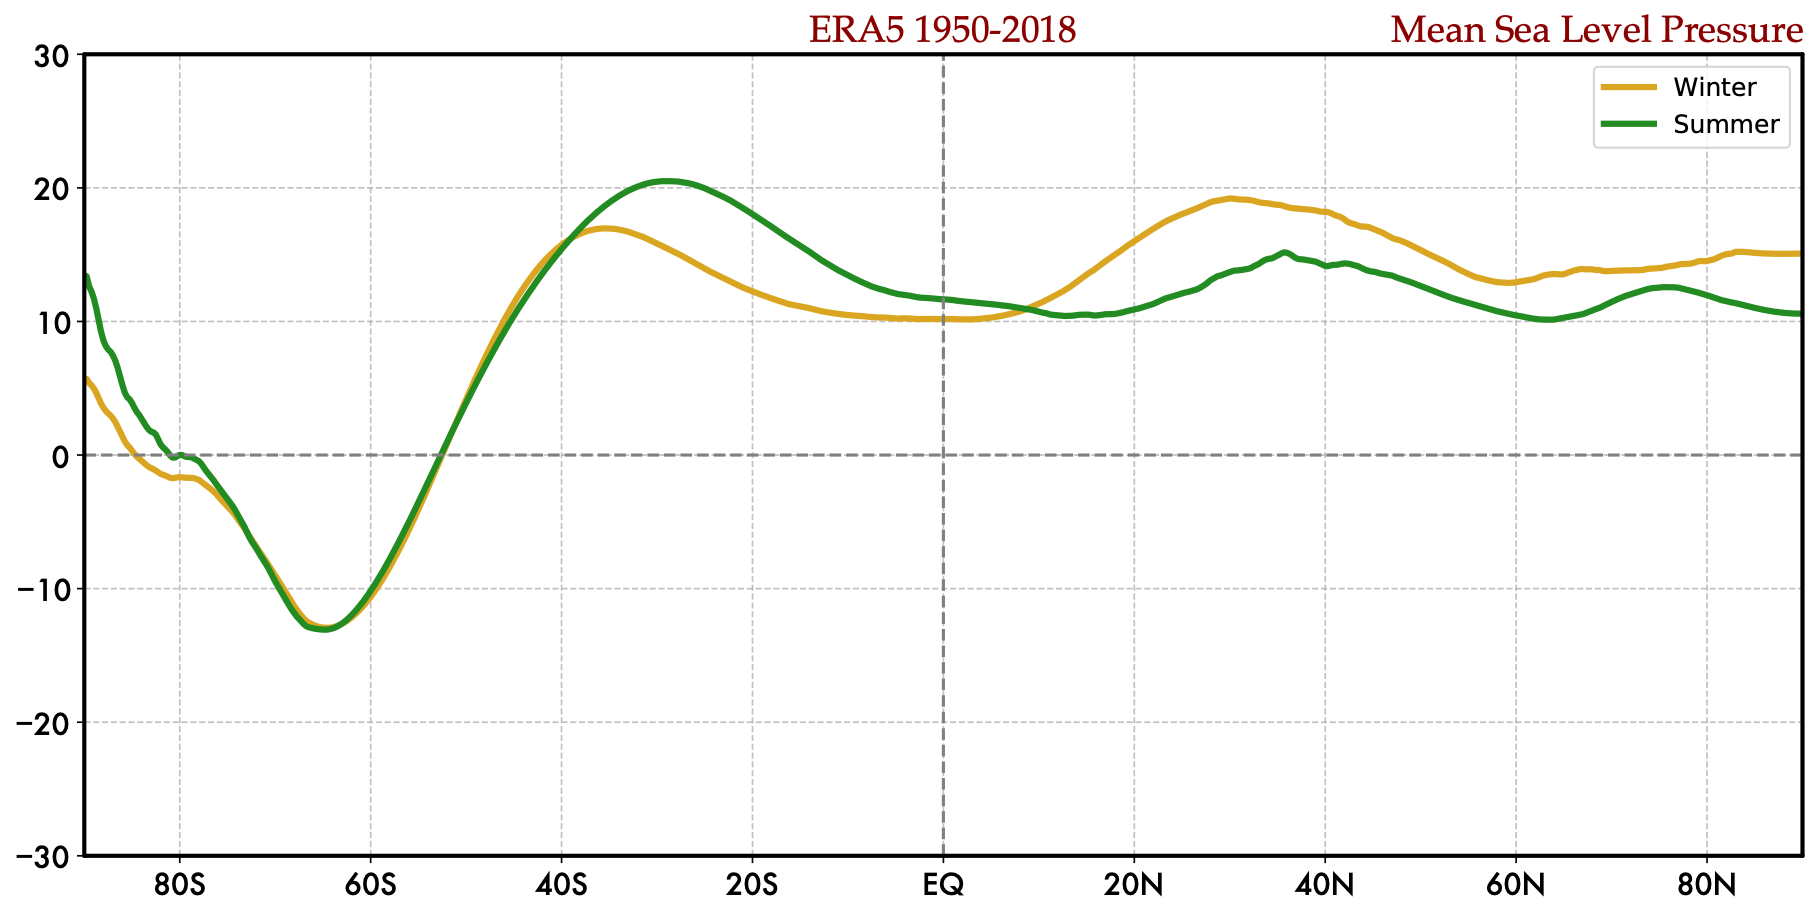
\includegraphics[width = .7 \textwidth]{figs/GD/MSLZONALLDJF.png}
\caption{}\label{}
\end{figure}

\subsubsection{The Sea Surface
Temperature}\label{the-sea-surface-temperature}

North-South gradients dominate the distribution of the Sea Surface
Temperature in both seasons (Fig. \texttt{fig:60}). Polar regions are
very cold and dominated by sea ice (not visible in this picture),
whereas the equatorial regions are generally very warm. However, there
are large deviation from the zonal symmetry close to the east cost of
continents. especially in the equatorial Pacific Ocean vast intrusions
of cold water are visible straight at the equator in the East Pacific,
where the water has the same temperature of the midlatitudes.

\begin{figure}
\centering
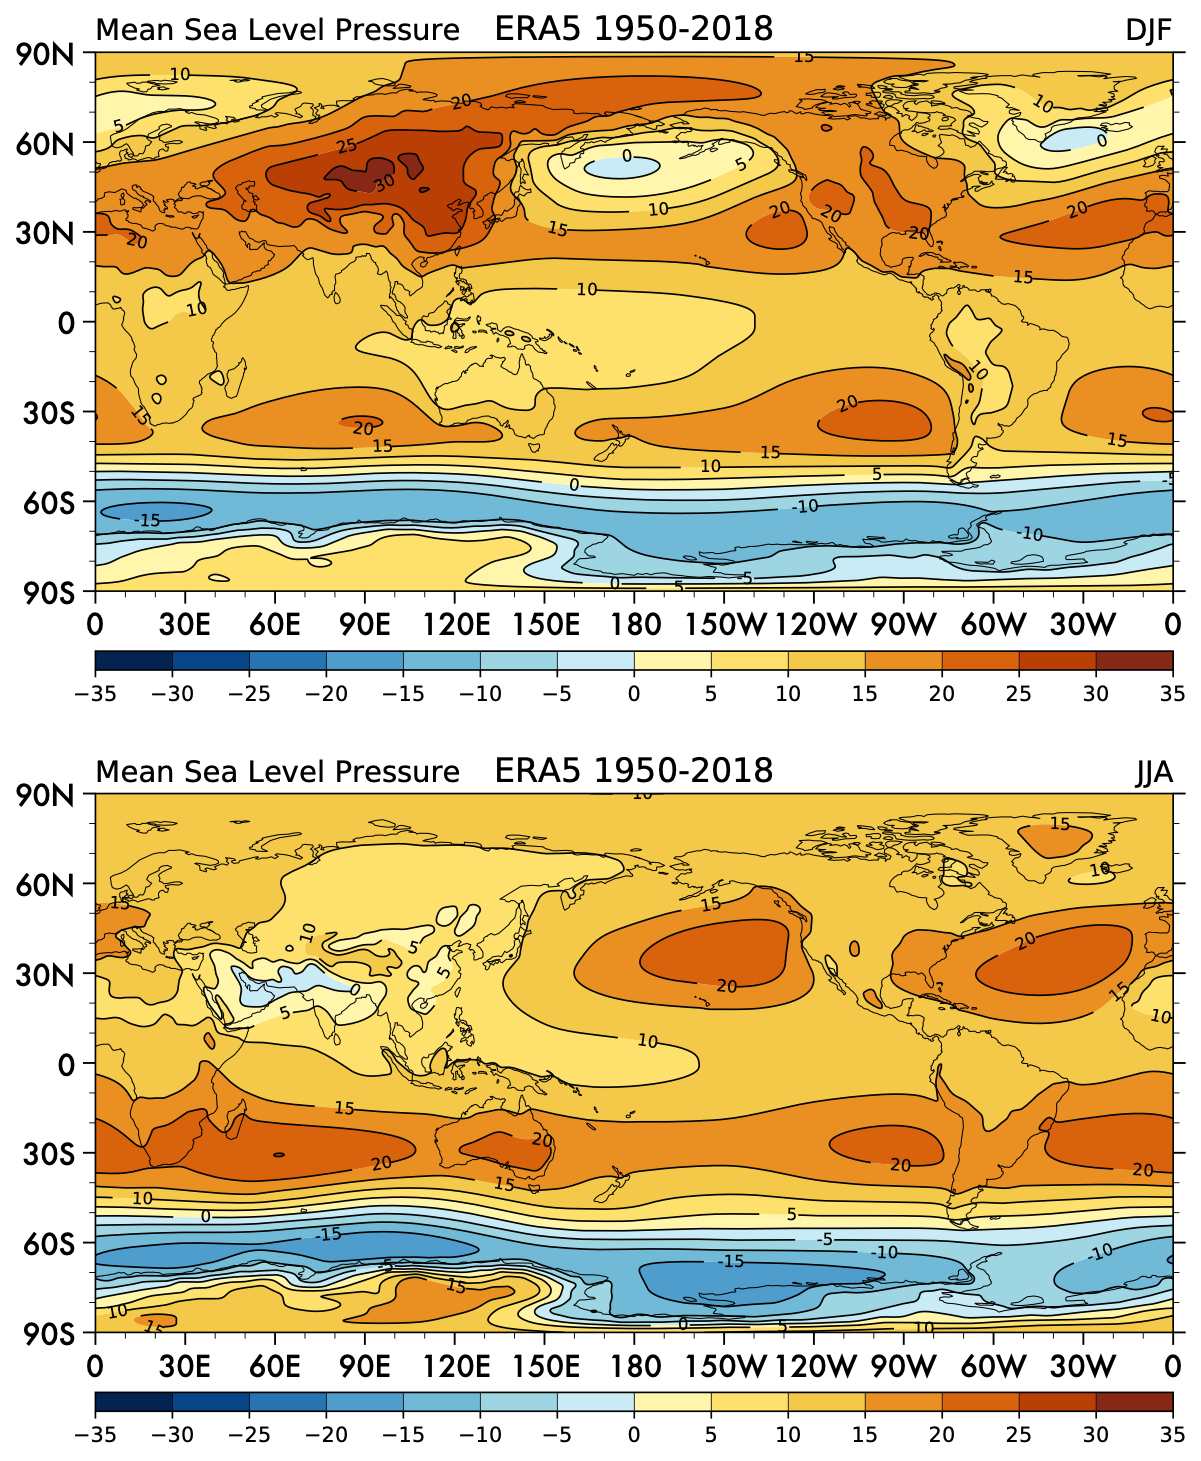
\includegraphics[width = .7 \textwidth]{figs/GD/MSL.png}
\caption{}\label{}
\end{figure}

This is in contrast with the West Pacific where a pool of very warm
water cover the entire region. it is clear that a large gradients exist
also at the surface along the Equator in the SST.

\begin{figure}
\centering
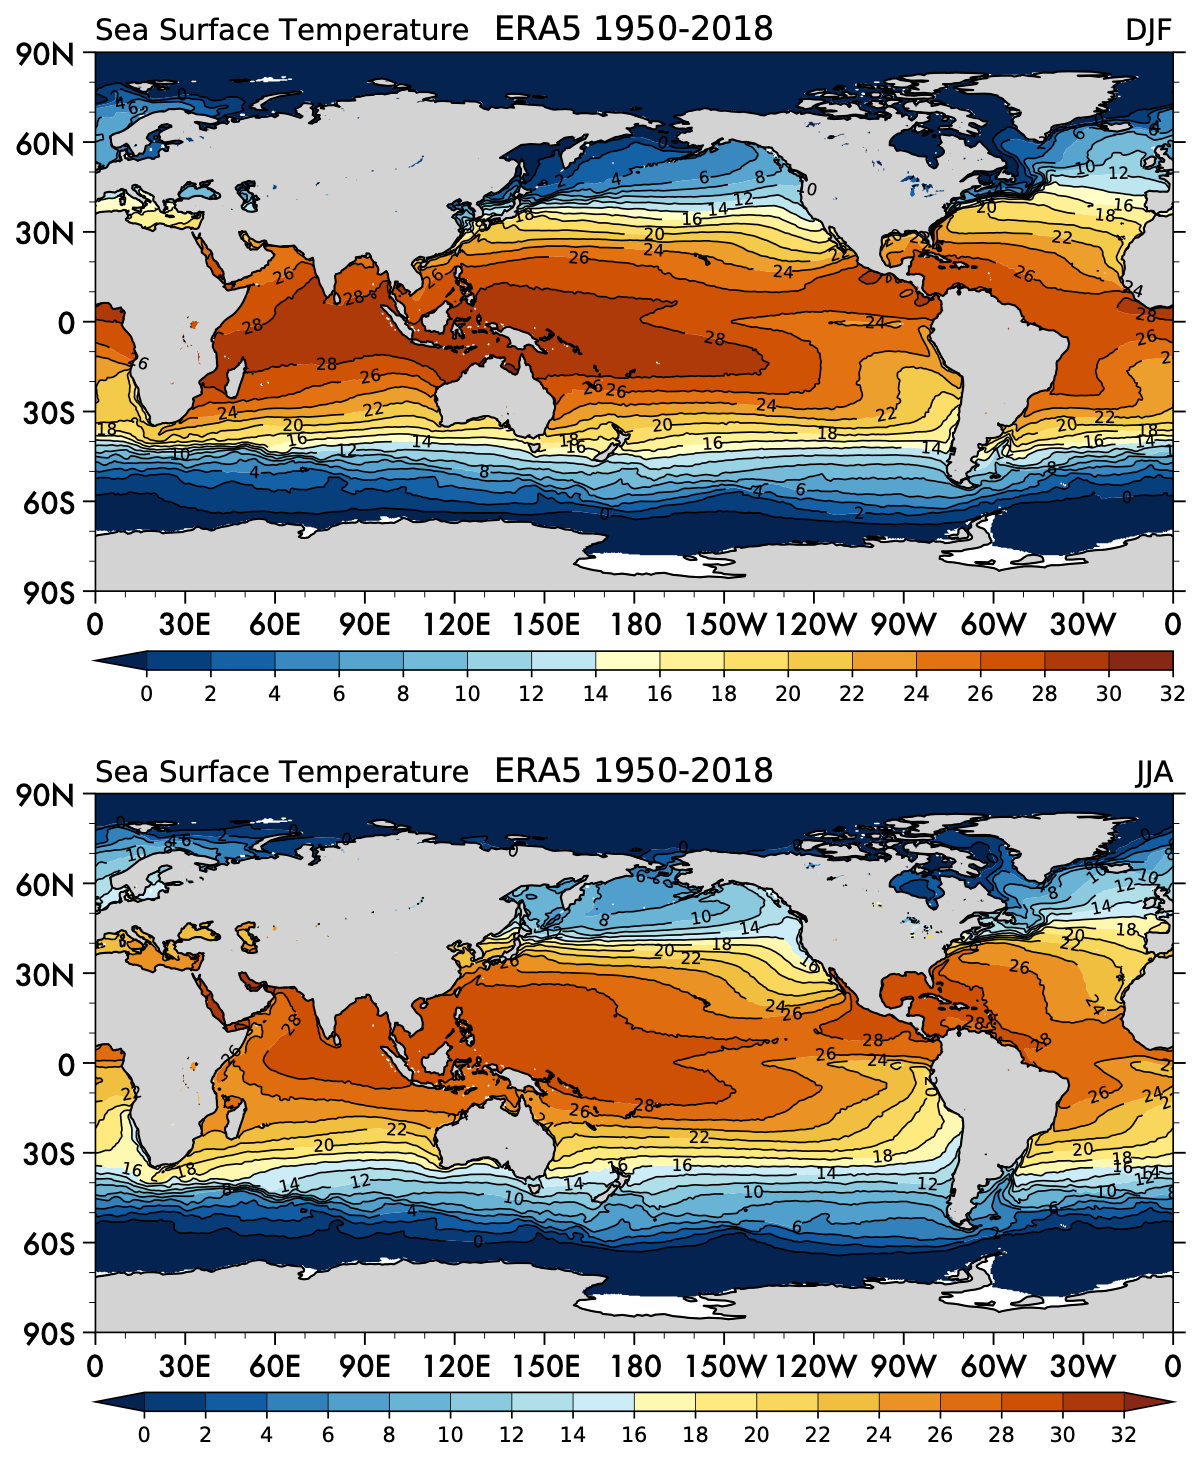
\includegraphics[width = .7 \textwidth]{figs/GD/SST.png}
\caption{}\label{}
\end{figure}

\subsubsection{The 2 Meter Temperature}\label{the-2-meter-temperature}

The SST show clearly the structure of the surface of the ocean, but it
is important to look also at near surface temperature for the entire
Earth surface. Land temperature will adjust very rapidly to the energy
balance and so it is usually used as a parameter of the surface
temperature the air temperature very close to the surfcae, usually
defined at two meter above the local surface. (Fig. \texttt{fig:602T})
show this temperature for Summer (bottom) and Winter (top). Over the
oceans it follows the SST as before, but over the continent it show a
strong seasonal variation. The northern continents are significantly
colder than the oceans at the same latitude. The West coasts of
continents is also relatively milder than the East Coasts.

\begin{figure}
\centering
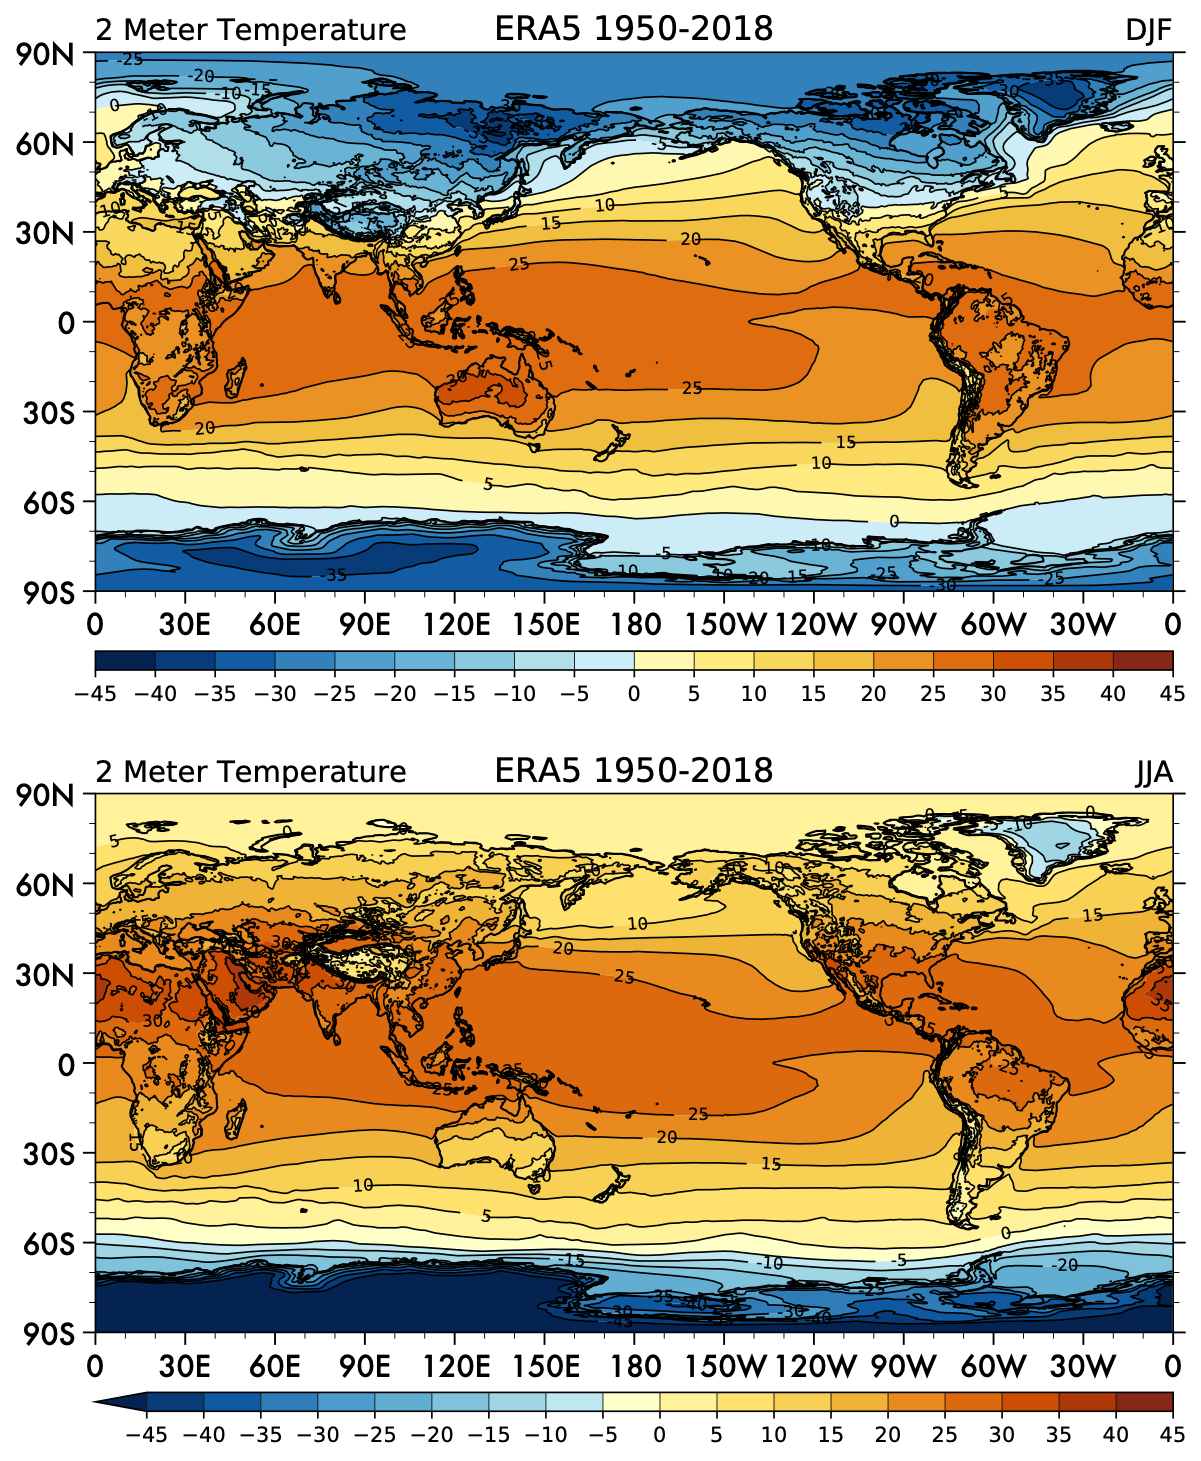
\includegraphics[width = .7 \textwidth]{figs/GD/2T.png}
\caption{Two Meter Air temperature for DJF (top) and JJA (bottom).}
\label{fig:}
\end{figure}

This is in contrast with the West Pacific where a pool of very warm
water cover the entire region. it is clear that a large gradients exist
also at the surface along the Equator in the SST.

\subsection{The Kinetic Energy}\label{the-kinetic-energy}

The total kinetic energy per unit mass can be defined as

\[K_T = \frac{1} {2} ( u^2 + v^2).\]

We can analyze the contribution of different components introducing the
splitting \((u = \bar{u}+ u', \cdots )\) for the time mean and similarly
for the zonal mean and following the arguments in Section
\texttt{Sect:Higher}, we get

\[K_T = \frac{1} {2}( [\overline{u^2} + \overline{v^2}])\]

where

\[\begin{aligned}
&K_{SE} =\frac{1} {2}( [(\bar{u}^*)^2]  + [(\bar{v}^*)^2]) \qquad & \text{Stationary Eddies}\\
& K_{TE} = \frac{1} {2}( [\overline{u'^2}]  +[\overline{v'^2}] ) \qquad & \text{Transient Eddies}\\
& K_{MME} = \frac{1)} {2}([\bar{u}]^2 + [\bar{v}]^2) \qquad & \text{Mean Meridional Circulation}
\end{aligned}\]

The largest contribution comes from the meridionally symmetric component
(\(K_{MME}\) -- top panel). This is consistent with the weaker eddy
stationary component in this region, resulting in a more symmetric,
almost annular jet. The dominance of this component of course is one of
the reason under the observation of the \emph{circumpolar jet} as the
basic paradigm of the global circulation.

We present in Fig. :numref\texttt{fig:705} the kinetic energy split for
DJF and JJA. The calculation has been performed on the monthly mean data
from ERA5 therefore the transient elements are to be understood as
transients with respect the monthly mean variation from one month to
another. The data are then averaged over the season.

The transients contribution (\(K_{TE}\) -- second panel) is localized at
the margin of the subtropical zone with a visible extension into the
midlatitudes, basically it is confined between 30N and 60N. It is also
to be noted that these statistics were computed from monthly means data
and therefore some transients is being smoothed by the monthly mean.
Once again we can see here the effect of choosing a particular averaging
period.

The next term \(K_{SE}\) represents the contribution to the kinetic
energy of the time mean (stationary) deviations from the zonal mean
(eddies). The contribution from the standing eddies is large, indicating
a strong tendency of the Northern Hemisphere to generate slow, coherent
eddy structures that tend to persist on the monthly time scale.

\begin{figure}
\centering
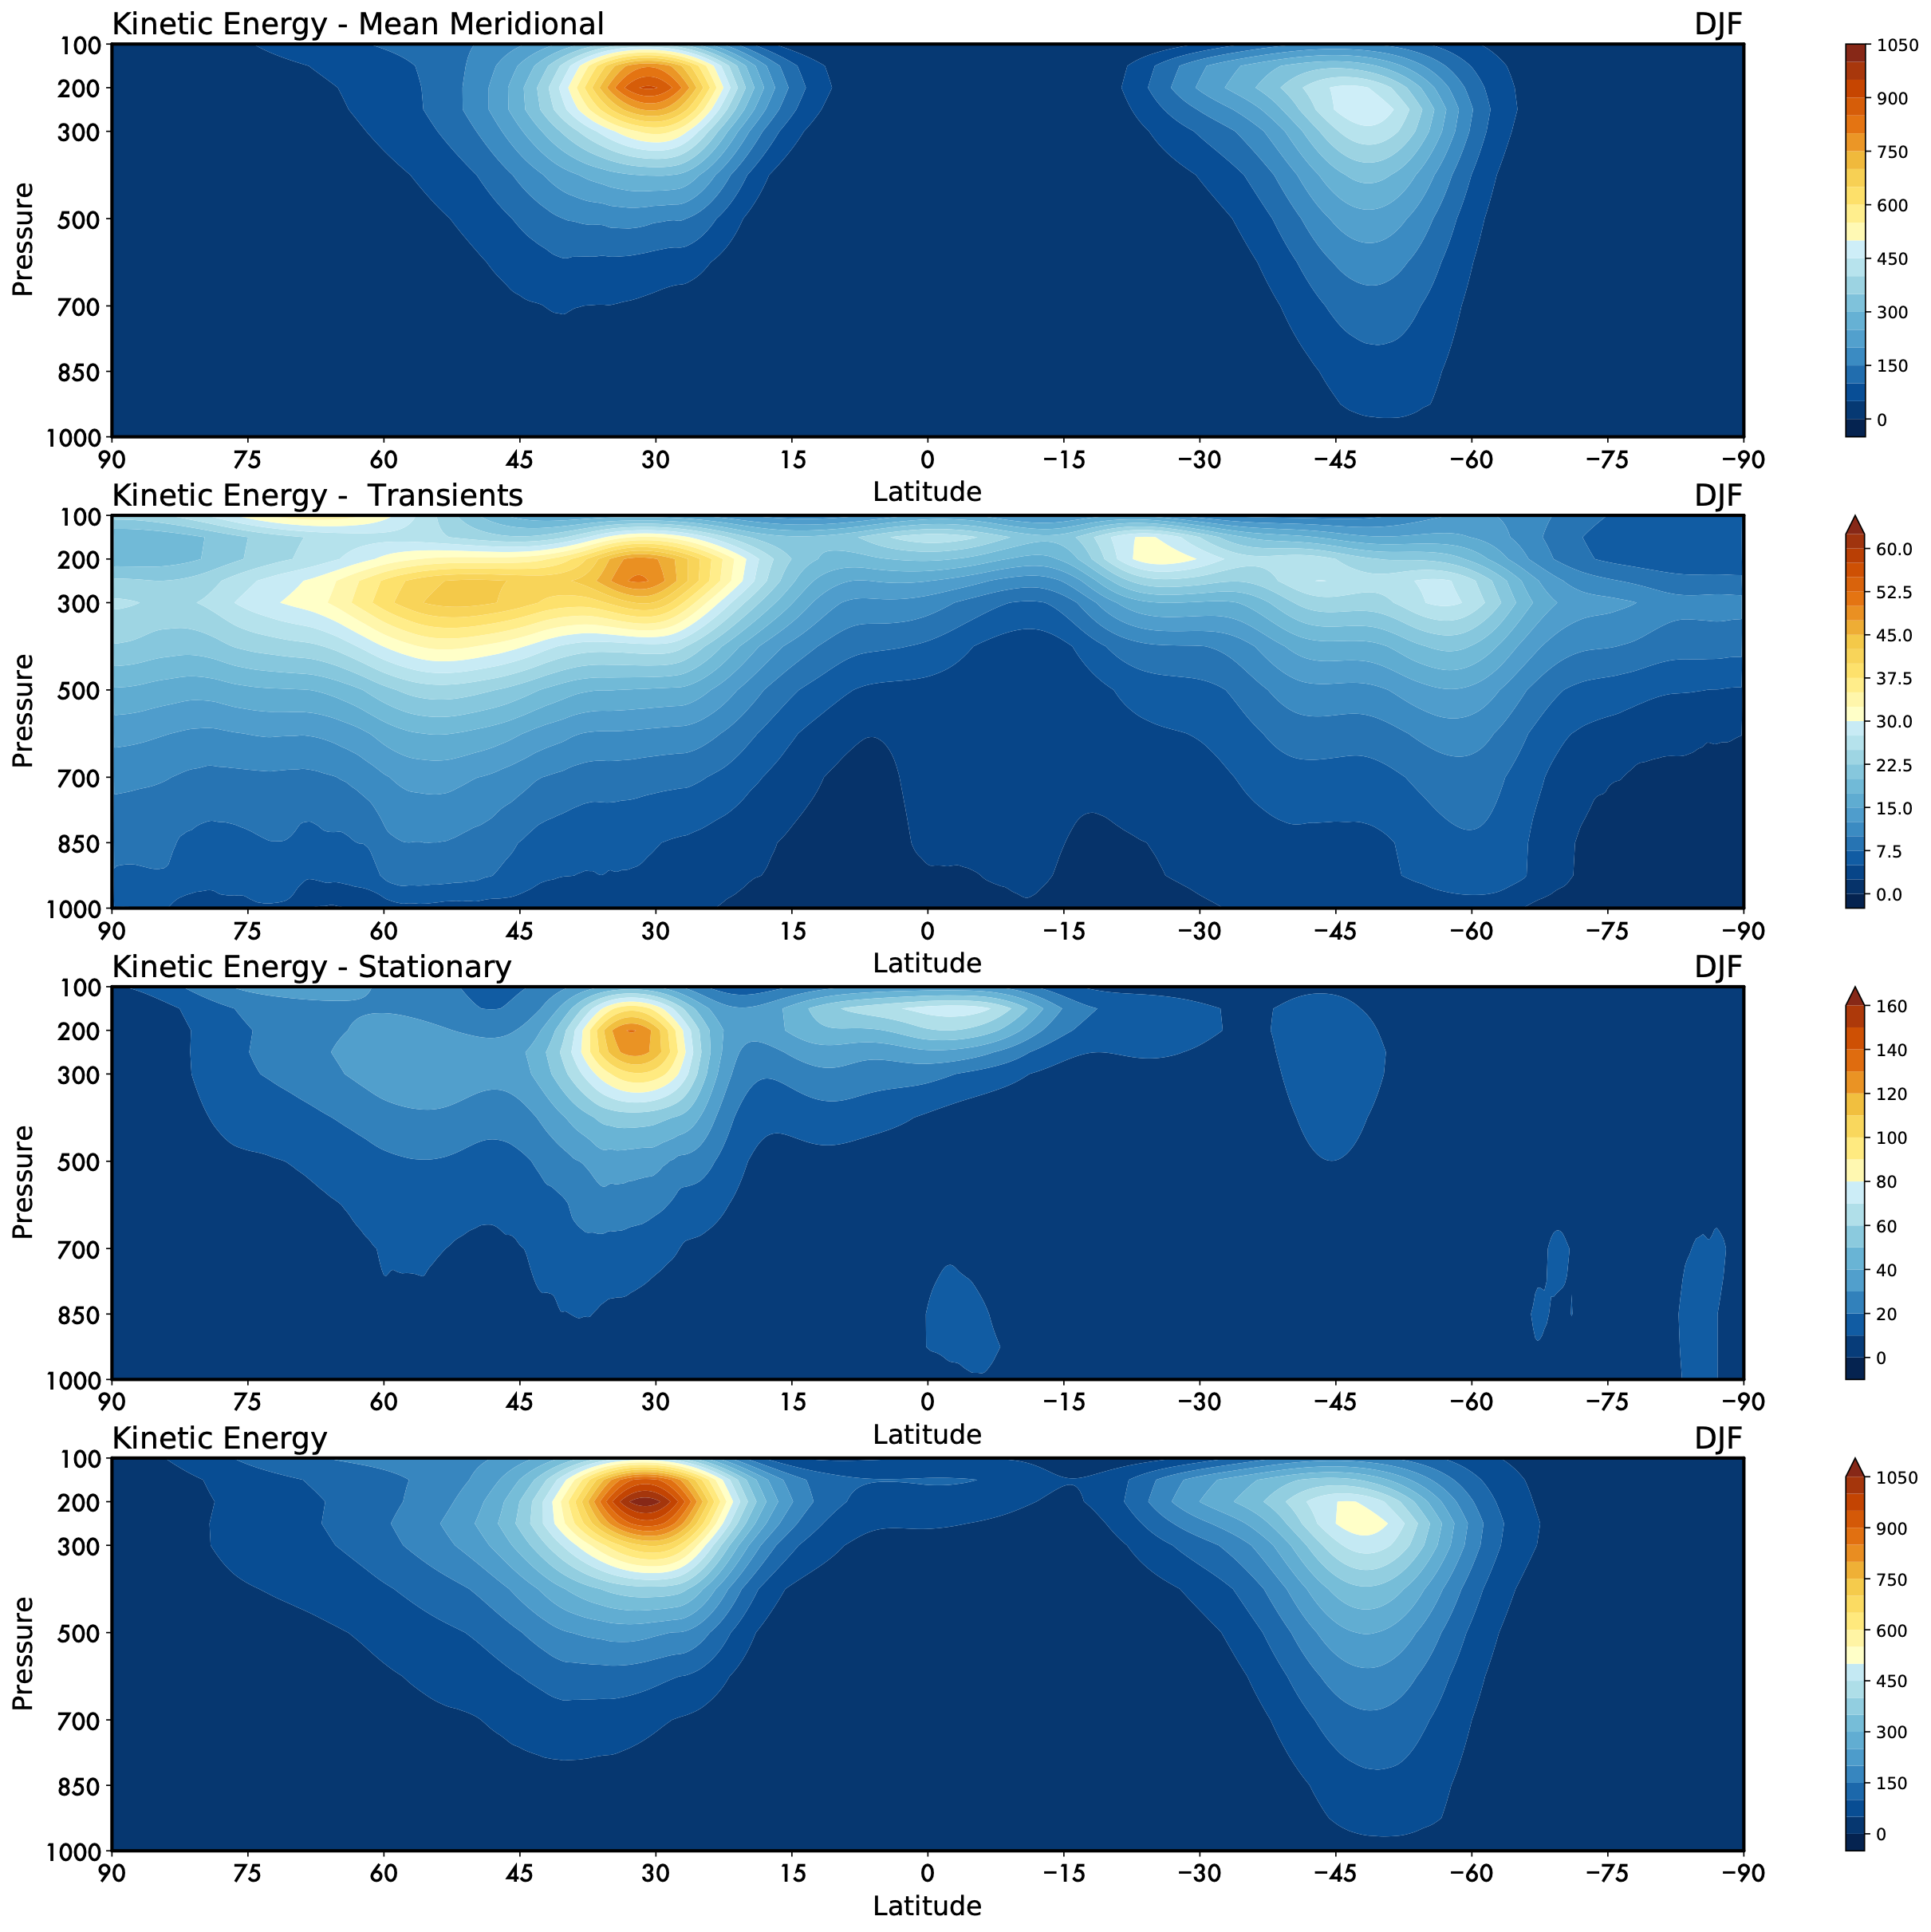
\includegraphics[width = .7 \textwidth]{figs/GD/DJFKEFlux.png}
\caption{}\label{}
\end{figure}

And finally the total kinetic energy \(K_T\) in northern hemisphere
Winter (bottom panel of Fig. \texttt{fig:70}) , shows a clear
correlation in the location of the zonal jets, both in latitude and
altitude.

\begin{figure}
\centering
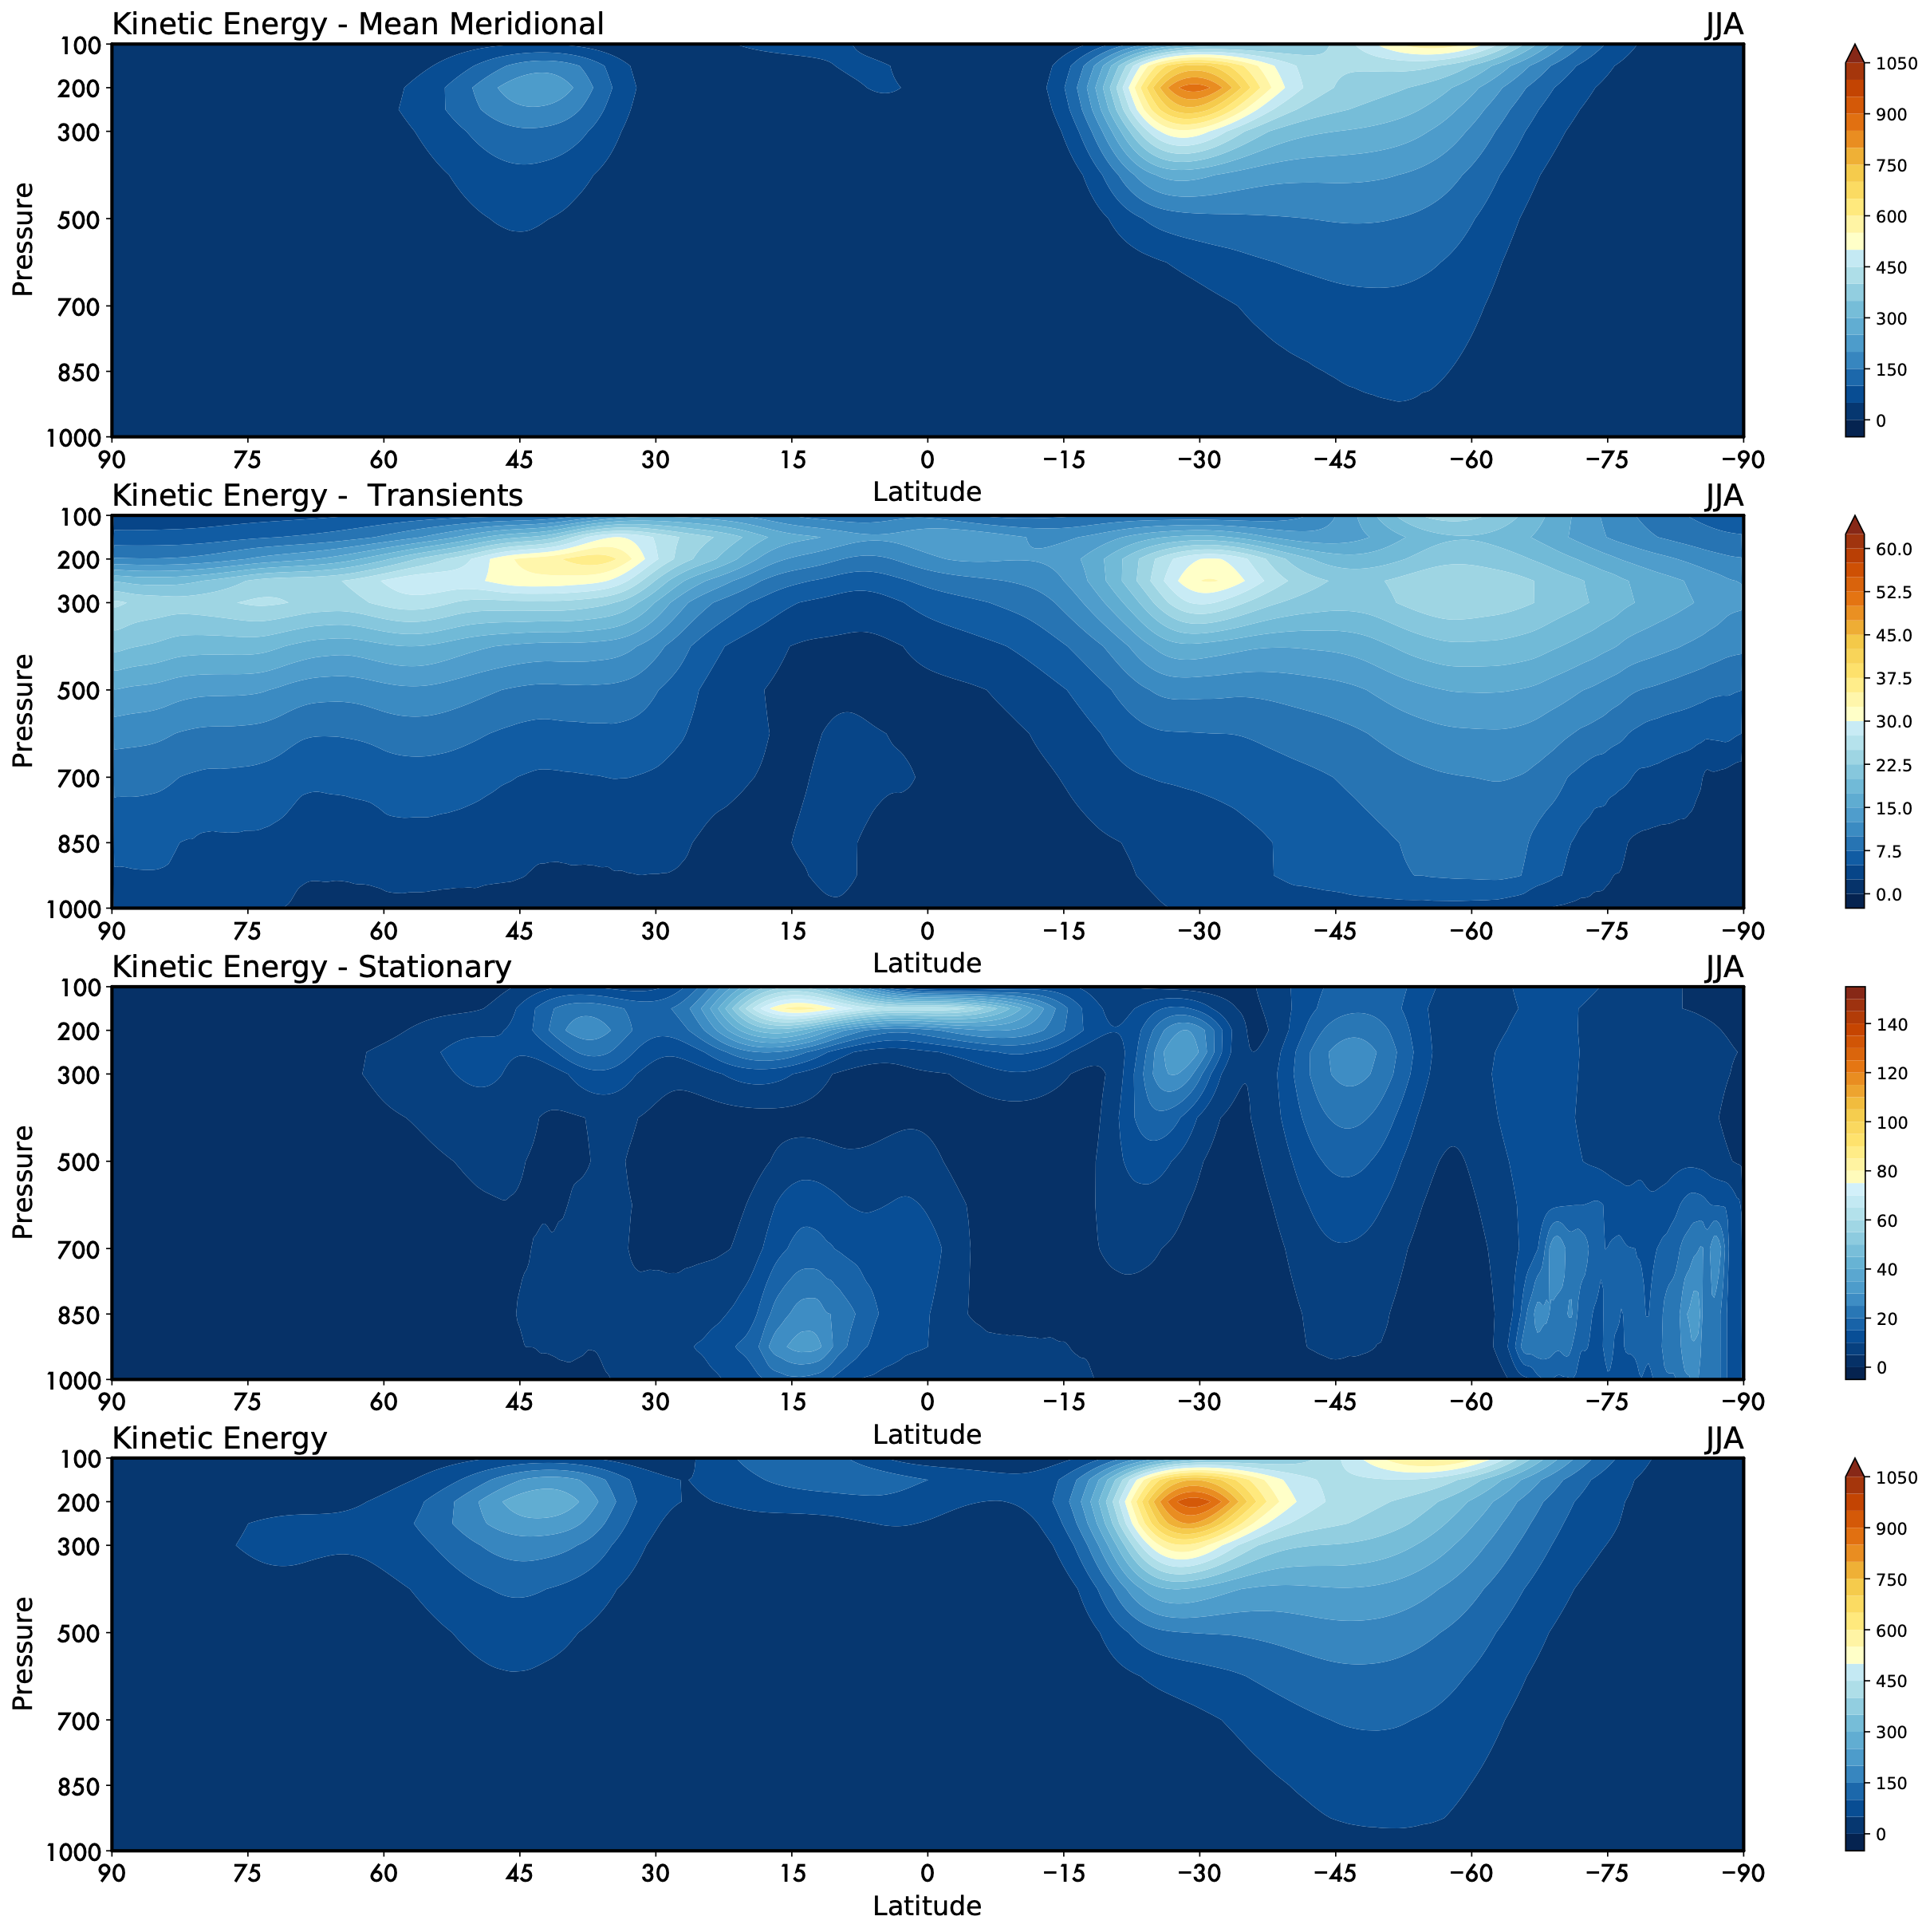
\includegraphics[width = .7 \textwidth]{figs/GD/JJAKEFlux.png}
\caption{}\label{}
\end{figure}

A similar situation is described in \texttt{fig:705} for JJA. Also in
this case the kinetic energy is colocated with the jet locations, but it
is possible to see that the standing eddies (third panel) are weaker
than in the Northern Hemisphereand a certain amount of transients is
still present in the Northern Hemisphere.

\subsection{The Meridional Momentum
Flux}\label{the-meridional-momentum-flux}

\begin{figure}
\centering
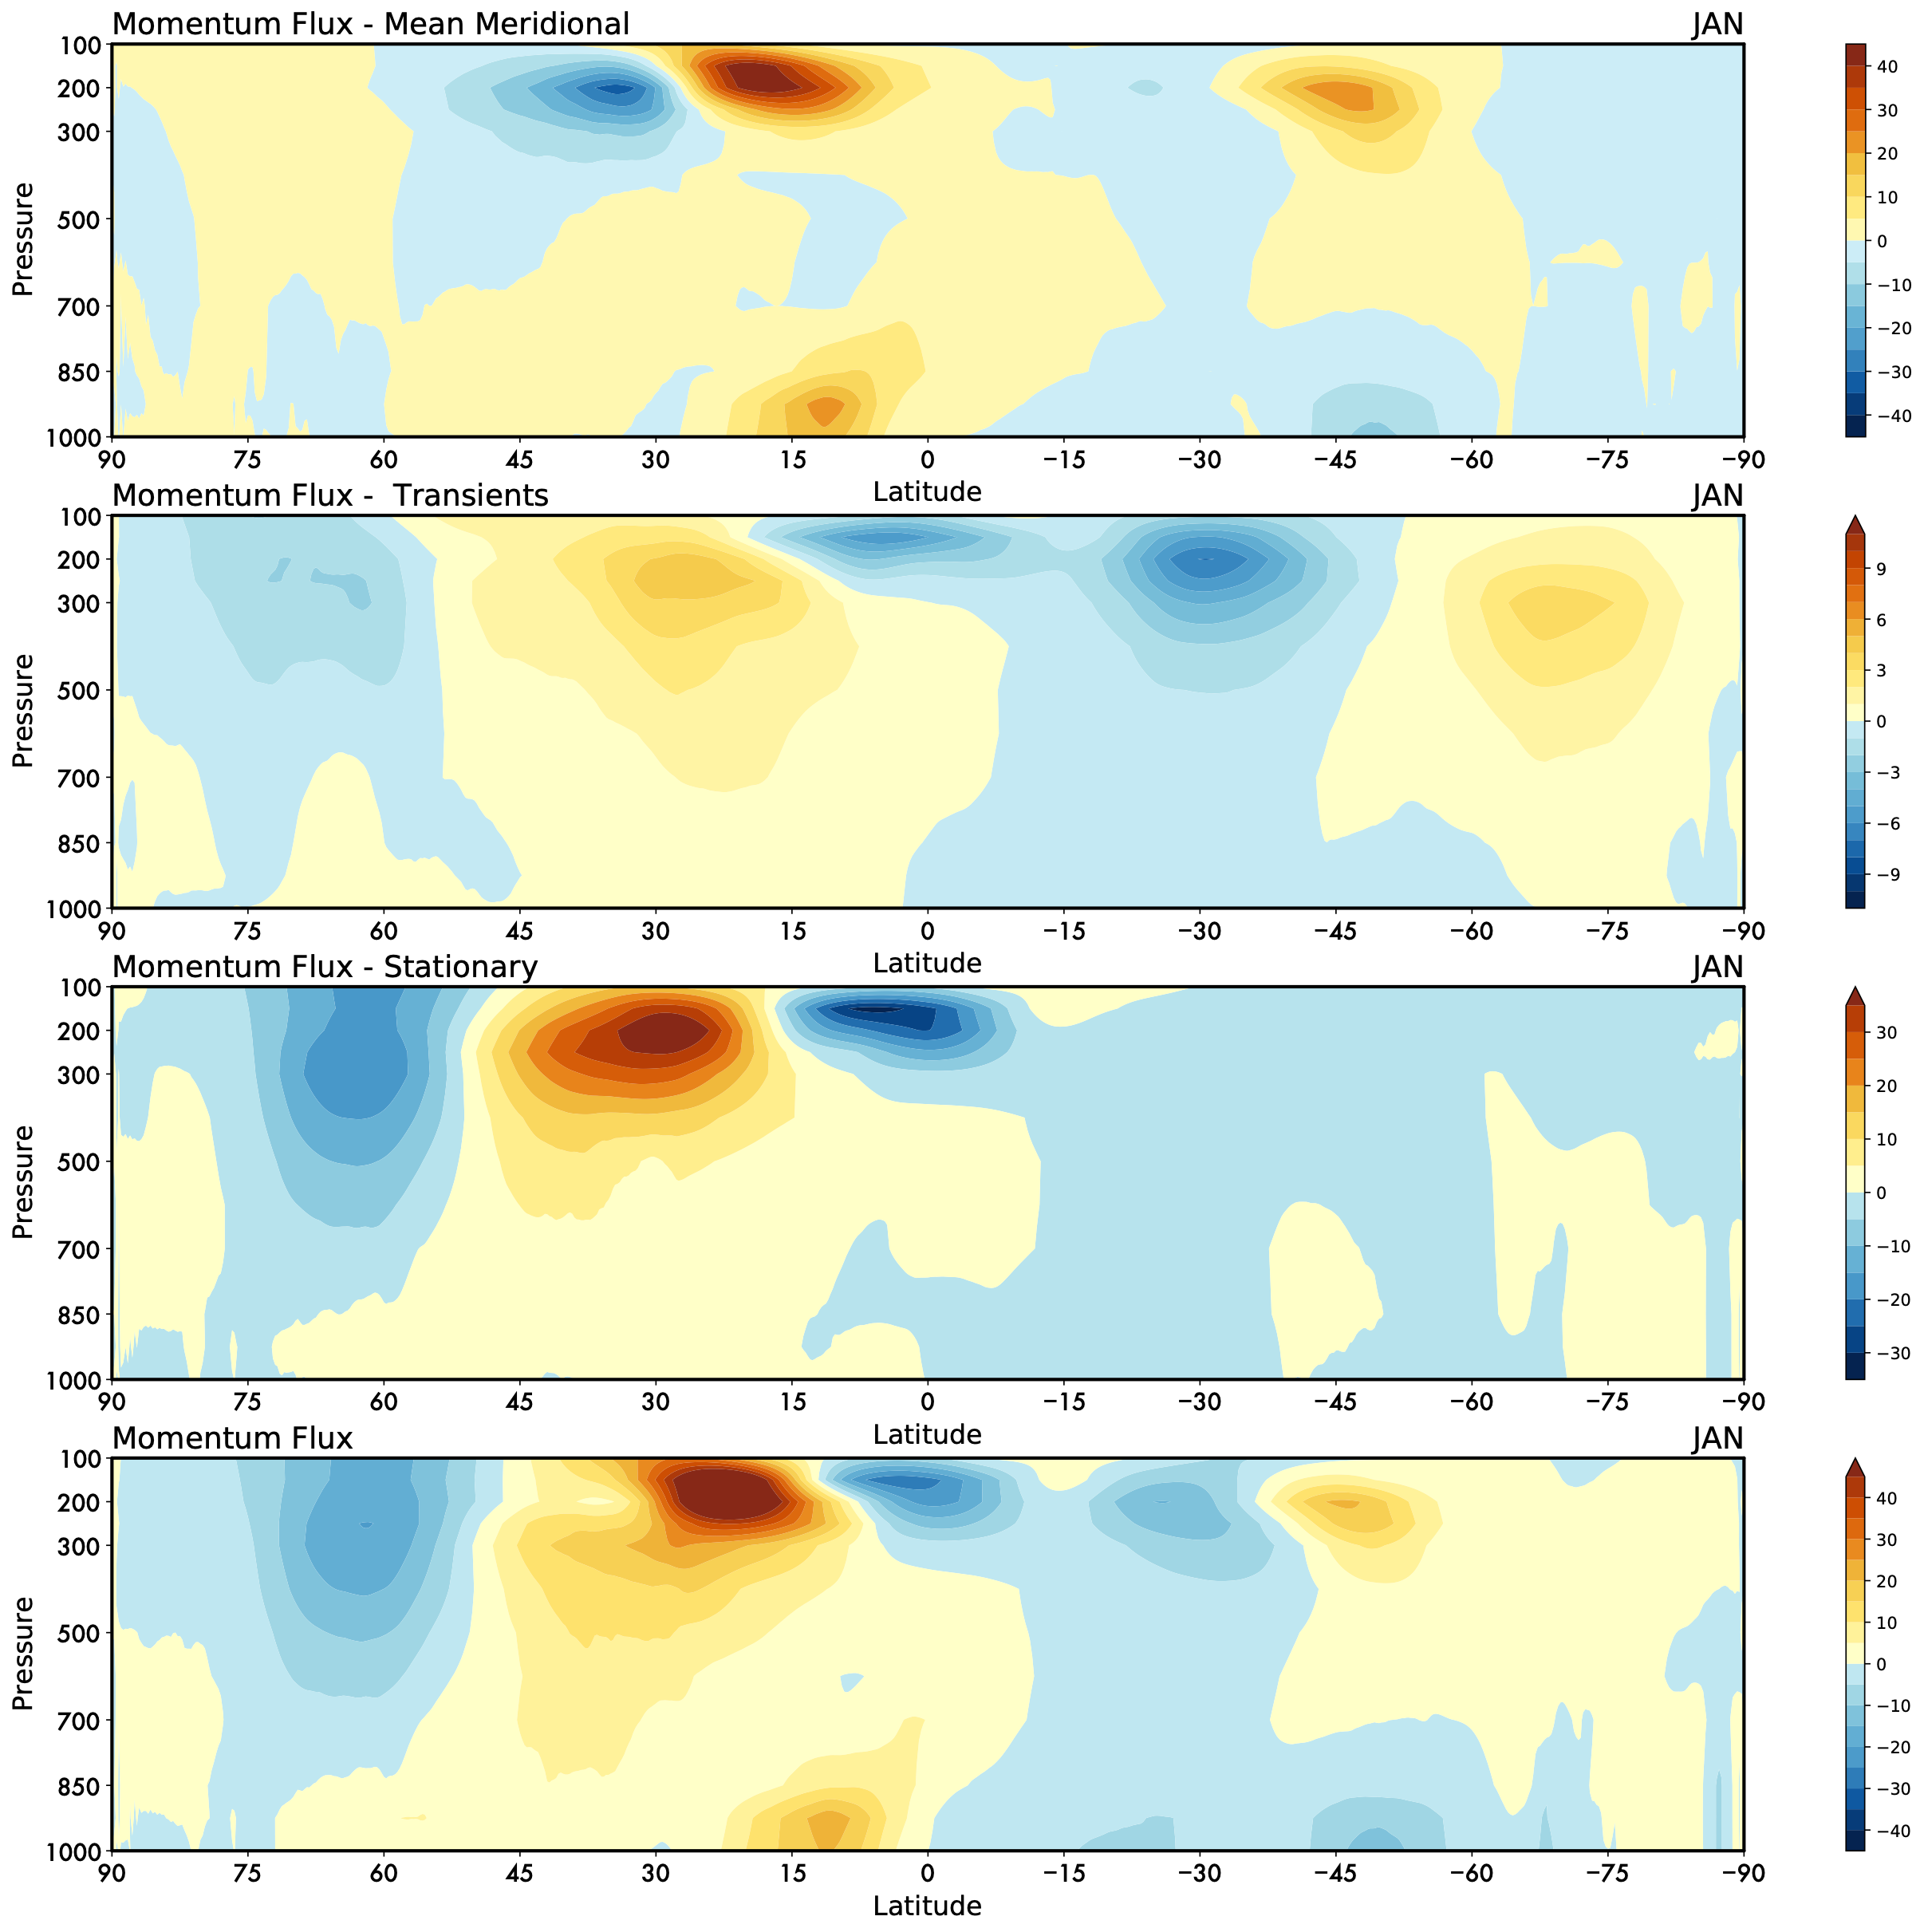
\includegraphics[width = .7 \textwidth]{figs/GD/JANUVFlux.png}
\caption{}\label{}
\end{figure}

\begin{figure}
\centering
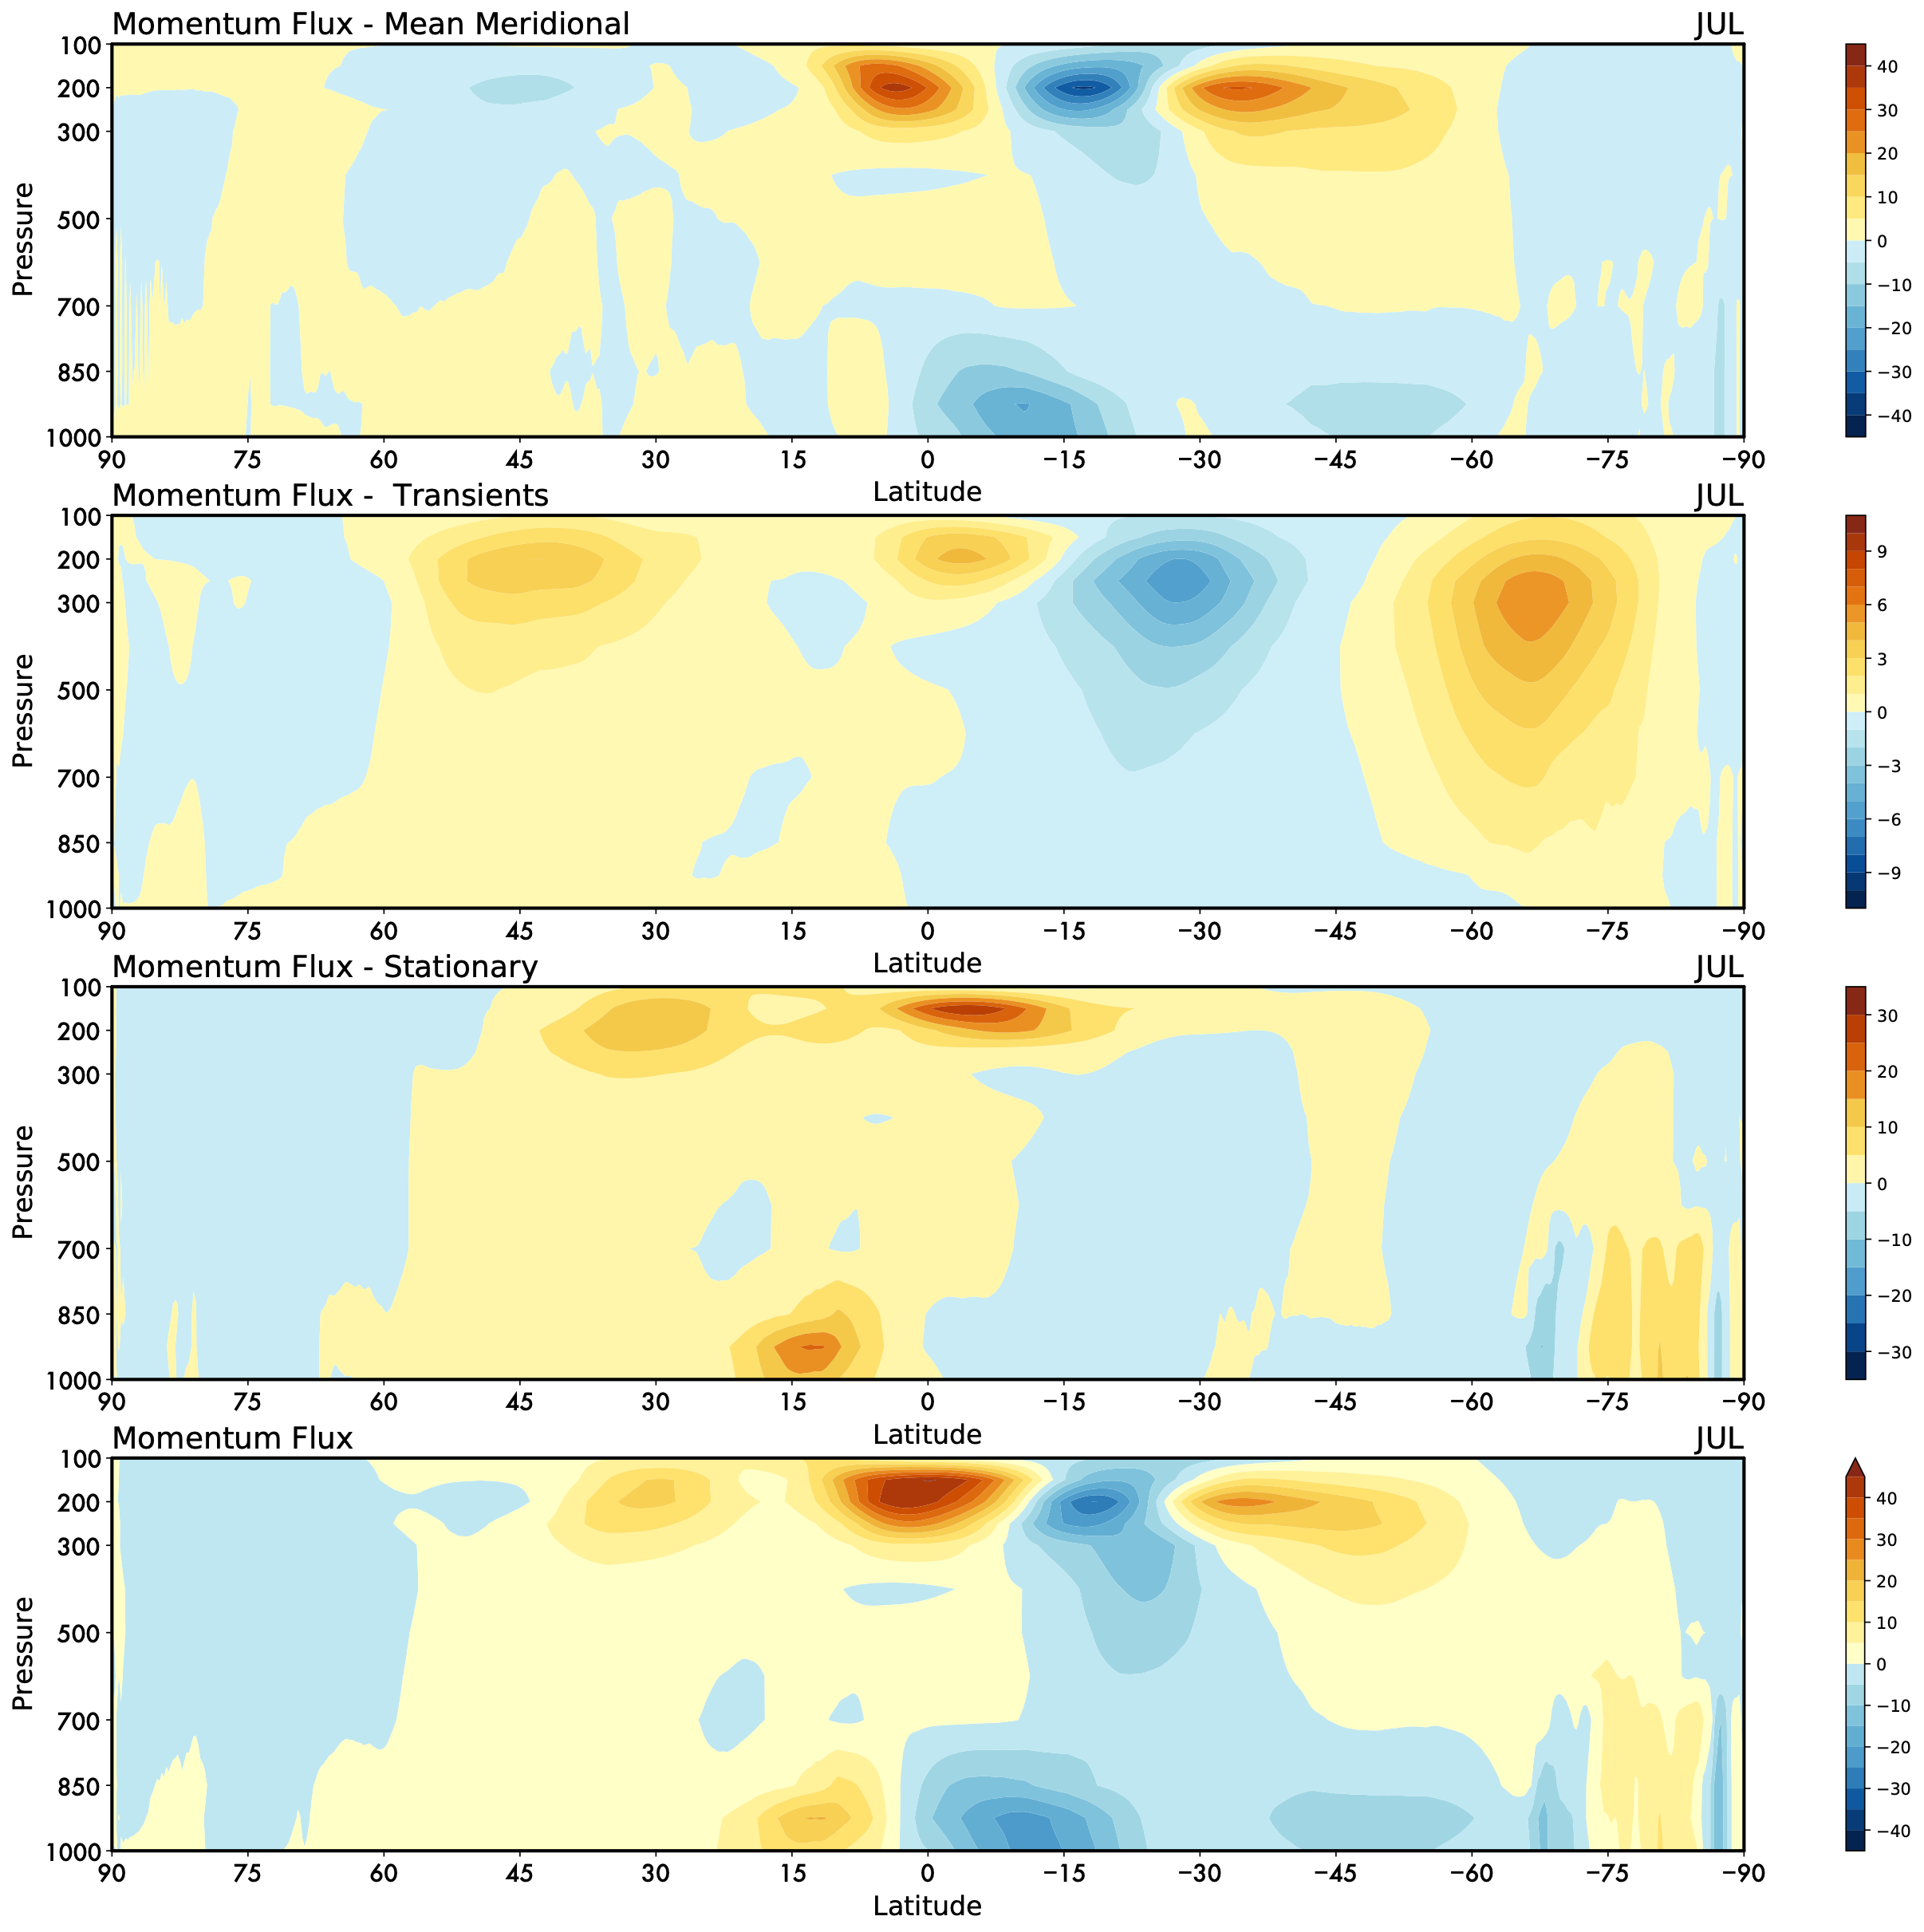
\includegraphics[width = .7 \textwidth]{figs/GD/JULUVFlux.png}
\caption{}\label{}
\end{figure}

\subsection{The Meridional Heat Flux}\label{the-meridional-heat-flux}

\begin{figure}
\centering
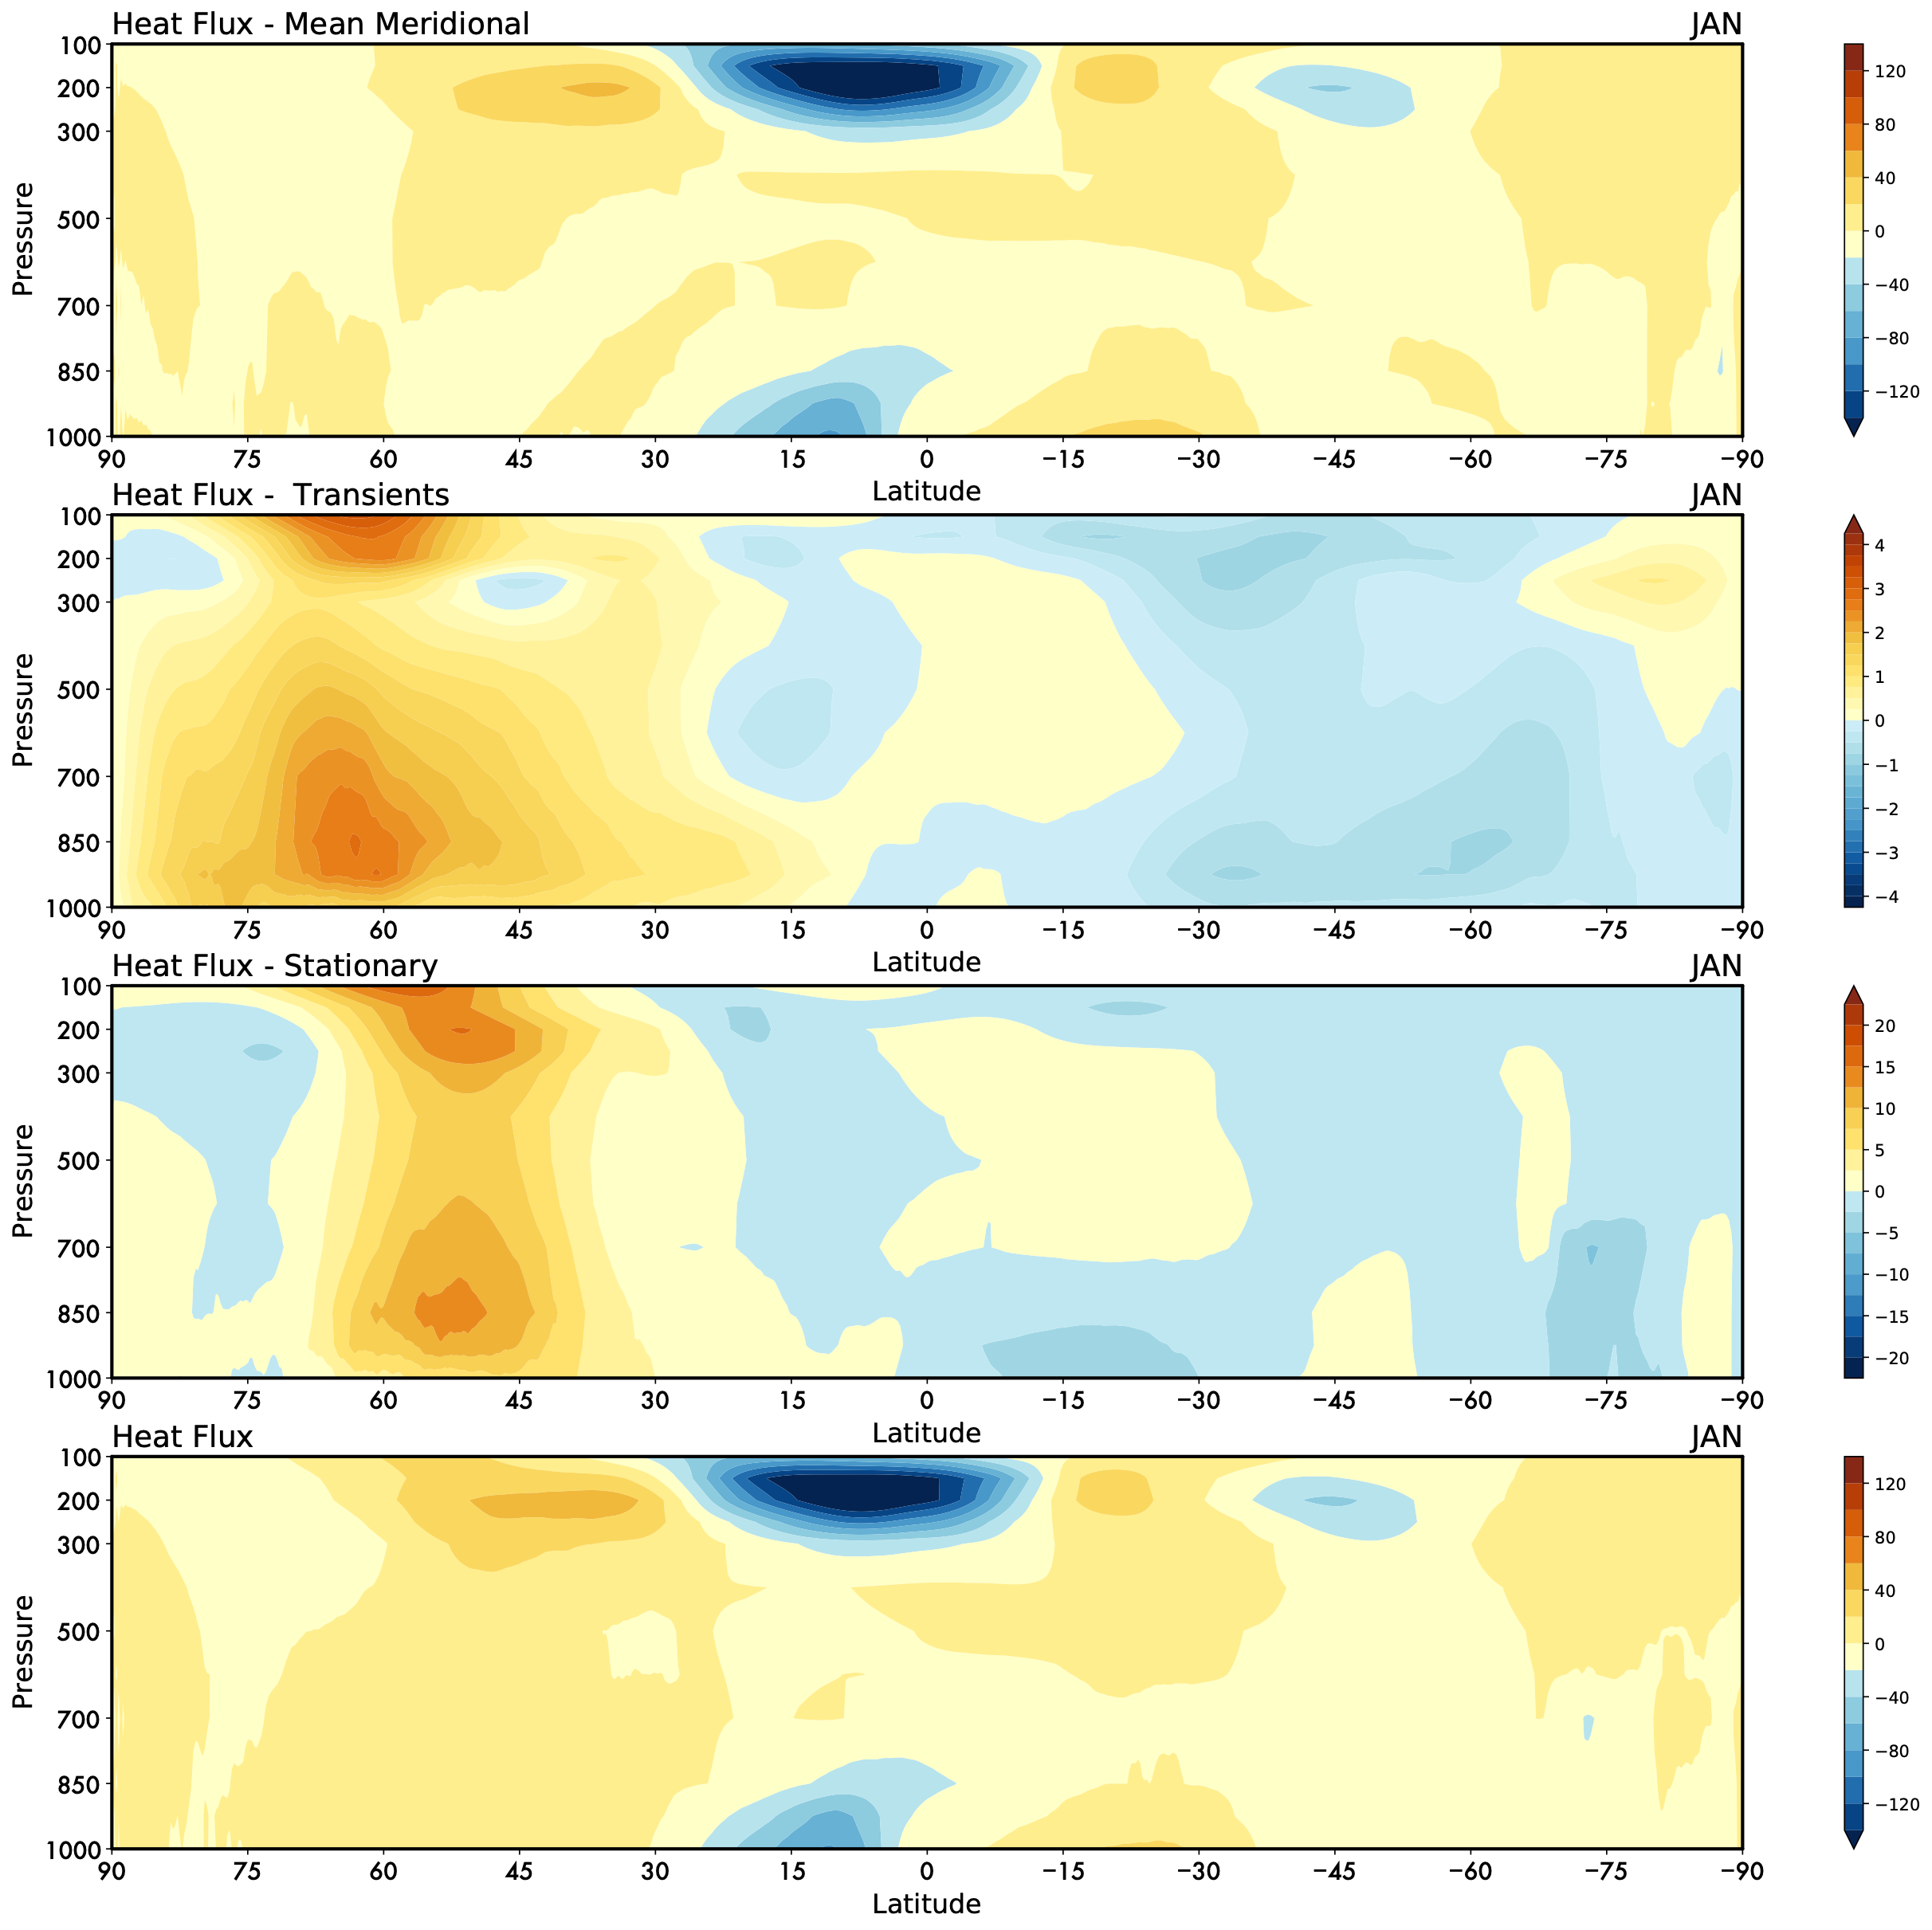
\includegraphics[width = .7 \textwidth]{figs/GD/JANTVFlux.png}
\caption{}\label{}
\end{figure}

\begin{figure}
\centering
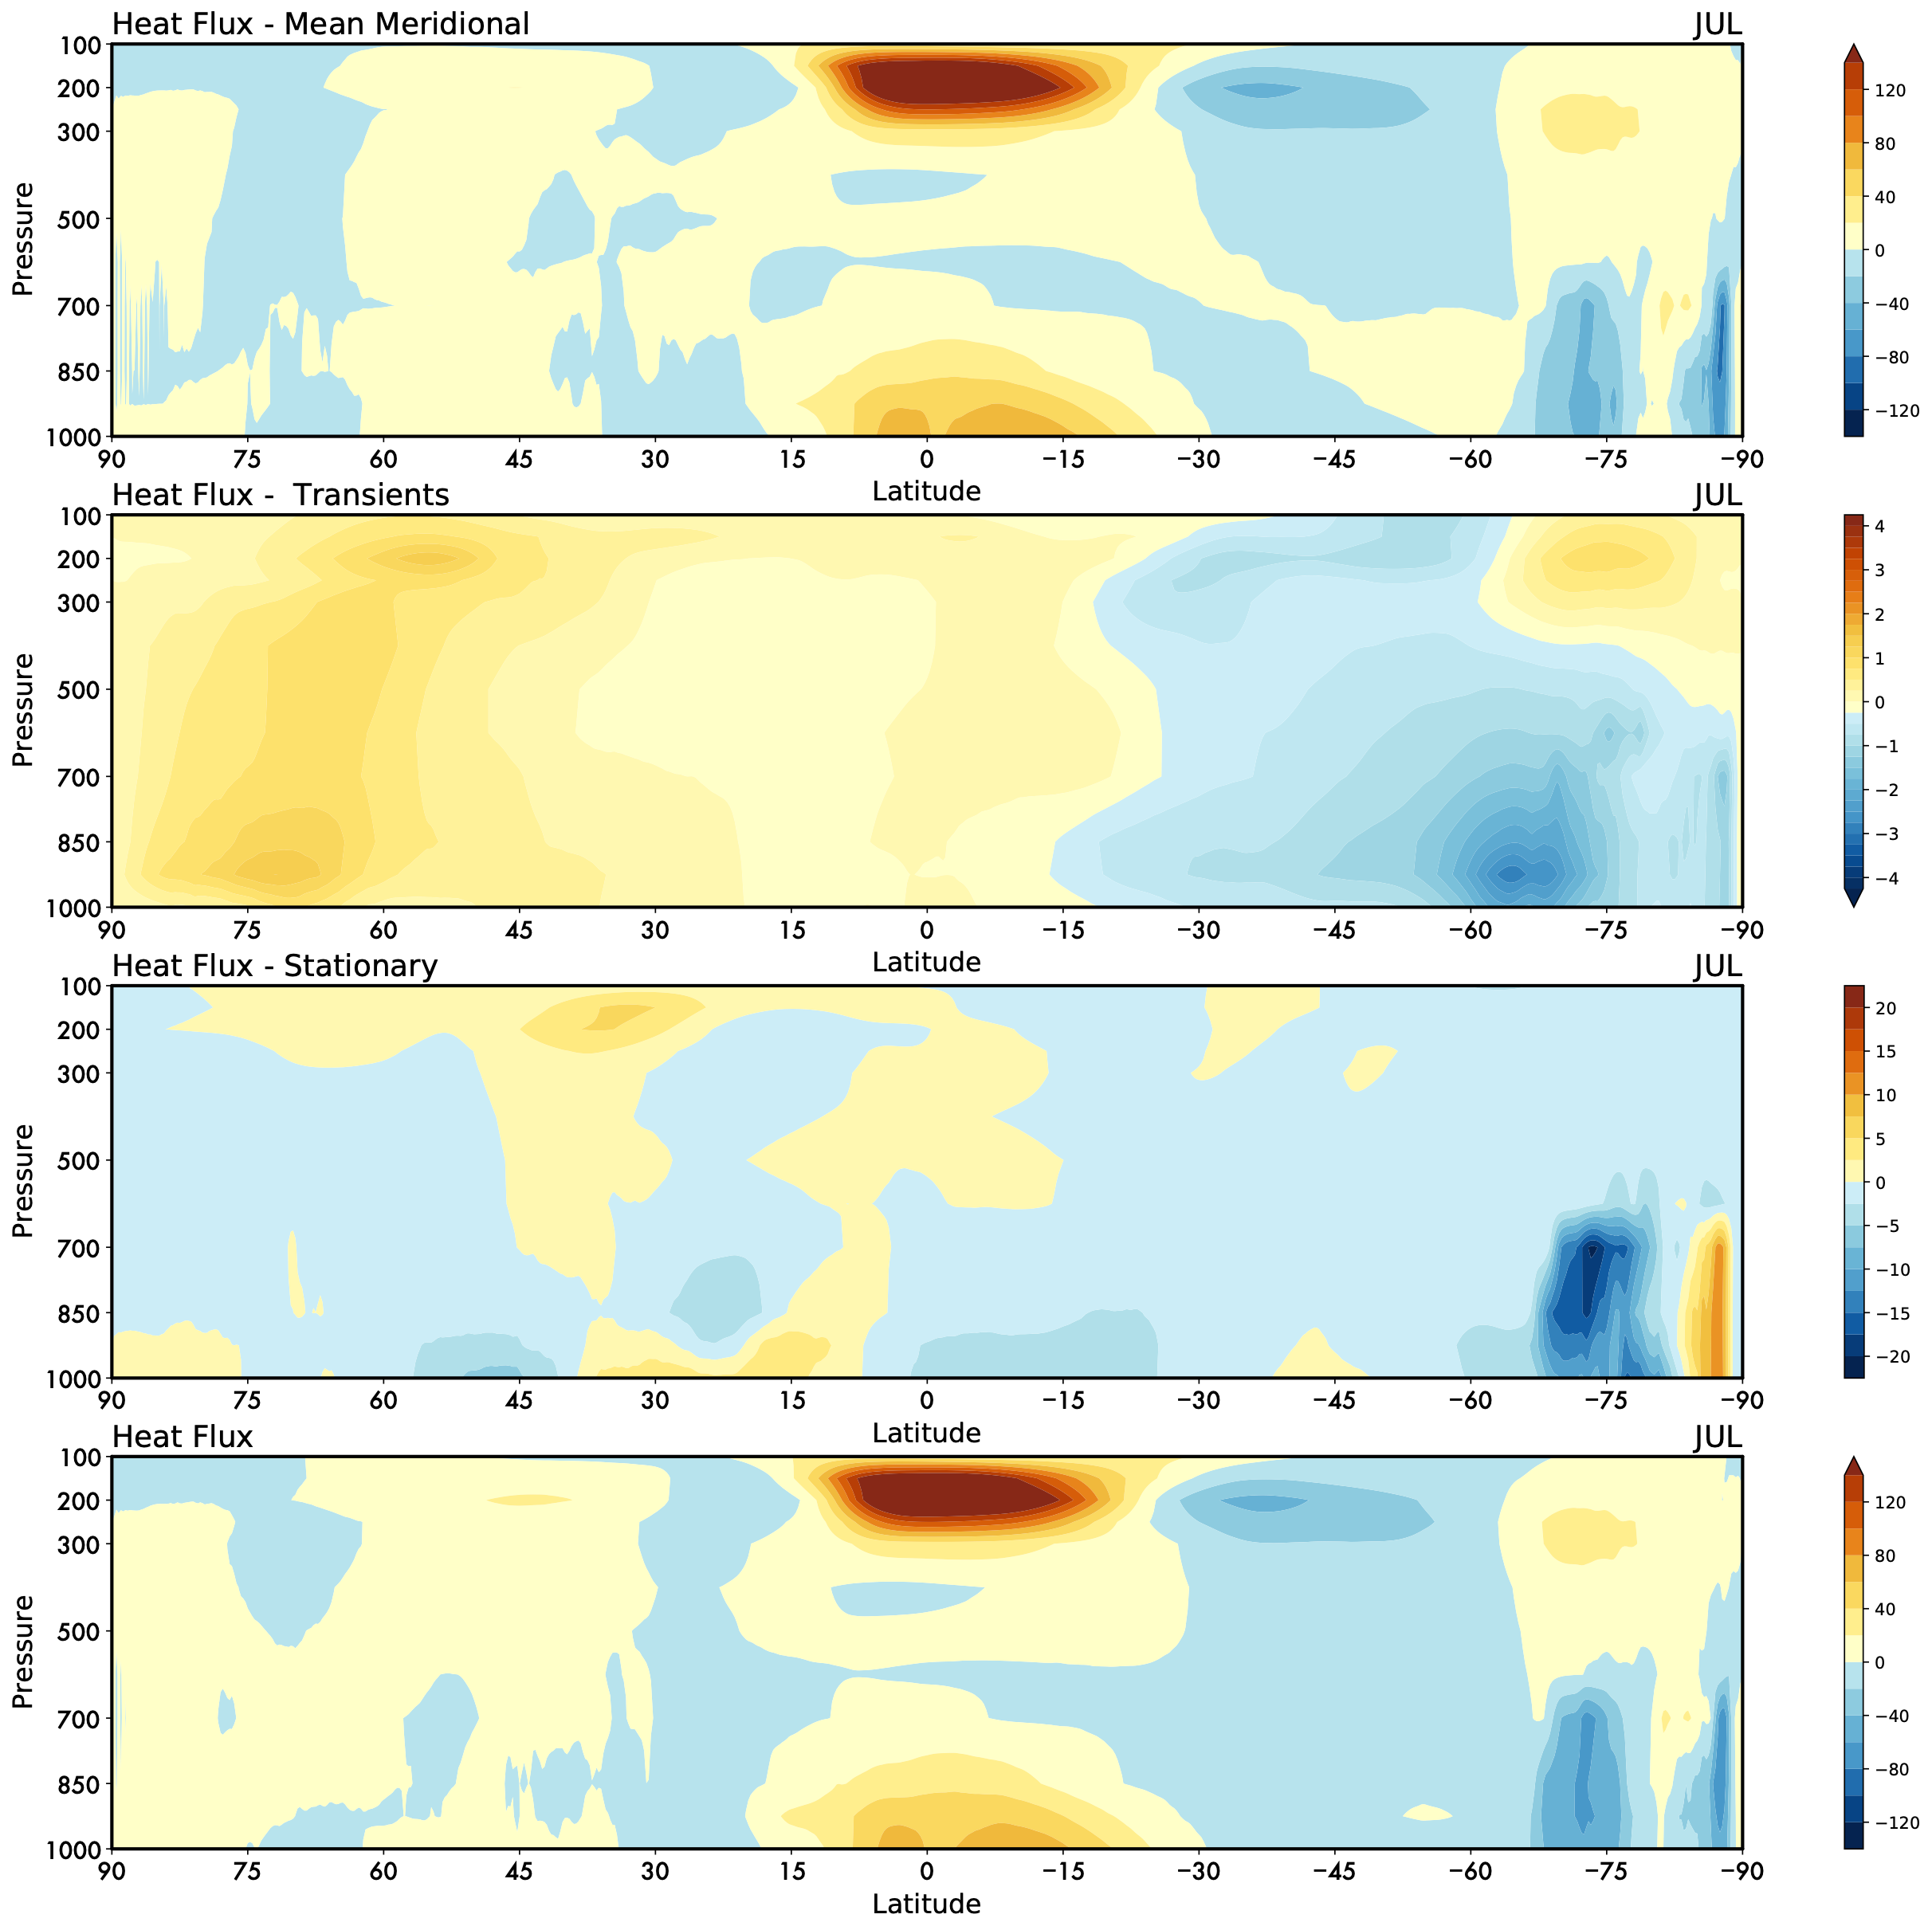
\includegraphics[width = .7 \textwidth]{figs/GD/JULTVFlux.png}
\caption{}\label{}
\end{figure}

The seasonal picture are in the appendix

    \section{The General Circulation of the
Oceans}\label{the-general-circulation-of-the-oceans}

The oceans show a general circulation similar to the atmospheric because
together they contribue to the equilibium energy balance of the planet.
The spherical symmetry of the atmosphere is lost because the presence of
the continents fragment the circulation and impose important constraints
on the circulation. On the other hand they are also a powerful system to
transfer momentum from the rotating solid planet to the fluid envelopes.
We will illustrate the ocean structure and circulation using the Global
Reanalaysis from cipollone2021teco that uses powerful methods to blend
observations and dynamical constraints to obtain a consistent picture of
the fields.

The ocean circulation is shaped by powerful forces, both dynamical and
thermodynamical. The energy balance at the surface has been shown in the
previous chapter, but the wind at the surface is certainly a dominant
factor. Fig. \texttt{fig:600} show the streamlines in both seasons of
the wind very close to the surface at the pressure level of 1000mb that
over the ocean is very close to the surface. The color is proportional
to the modulus of the wind vector, i.e. the speed.

\begin{figure}
\centering
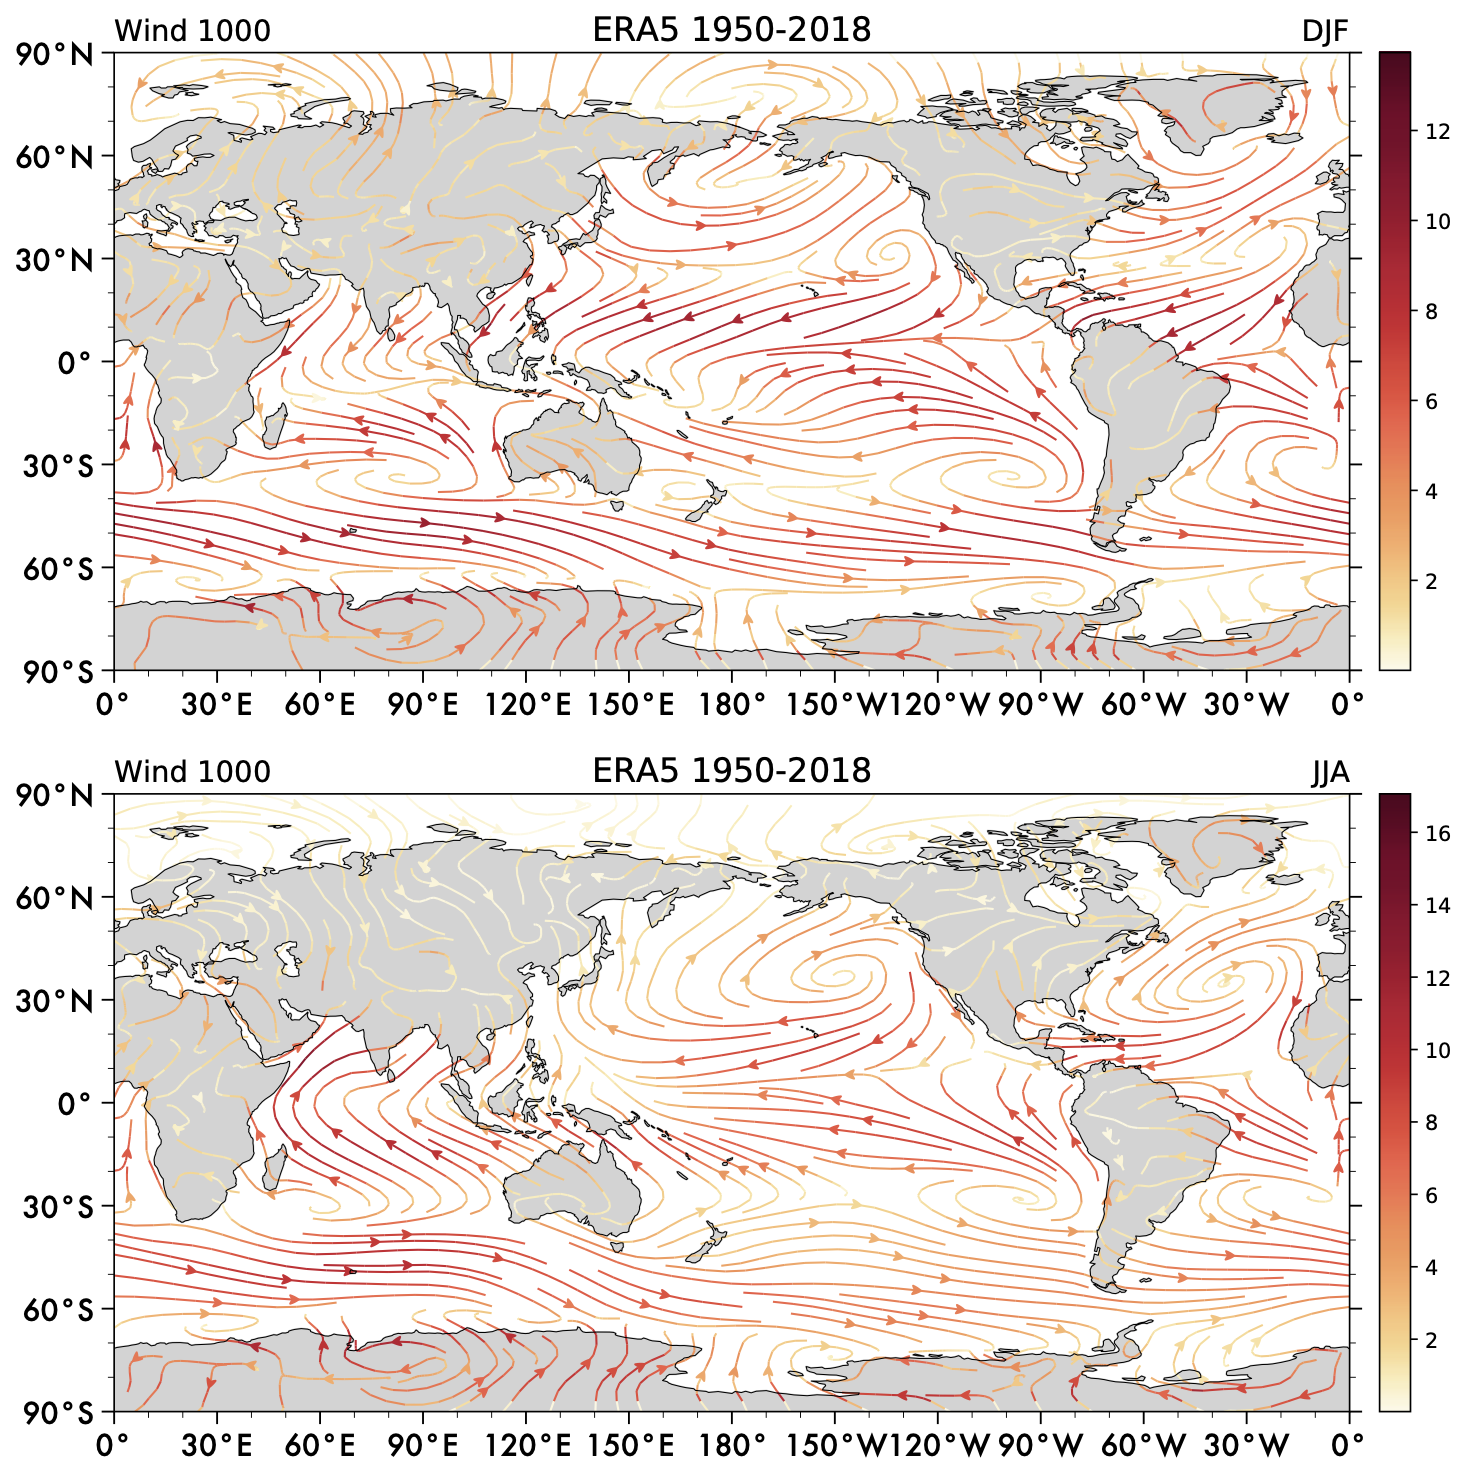
\includegraphics[width = .7 \textwidth]{figs/GD/Wind1000.png}
\caption{} \label{fig:}
\end{figure}

\subsection{The thermal structure of the
Ocean}\label{the-thermal-structure-of-the-ocean}

The temperature structure of the oceans is shown in Fig.
\texttt{fig:610}. The top panel shows the temperature near the surface
at a nominal depth of 5m. We notice that there is a strong latitudinal
gradient as the equatorial zone tends to have warmer temperatures and
colder areas develop towards the polar areas. It is simple to connect
this structure with the radiation balance indicating a positive balance
in the equatorial zone and a negative one in the polar regions.

However, the latitudinal structure is broken in several areas. There are
significant gradients along the Equator both in the Pacific and in the
Atlantic basins and in general the East side of the basin tend to be
colder than the West side. Furthermore significant cold area exist along
the Equator in the Pacific in the East and along the South American
coast. A careful analysis shows that also in the midlatitudes there are
strong East-West differences, as the East side of the basins tend to be
warmer than the West. And just to avoid confusion we have to become
familiar with the fact that the East side of an ocean basin is bordering
with the \emph{West coasts} of the respective continent.

\begin{figure}
\centering
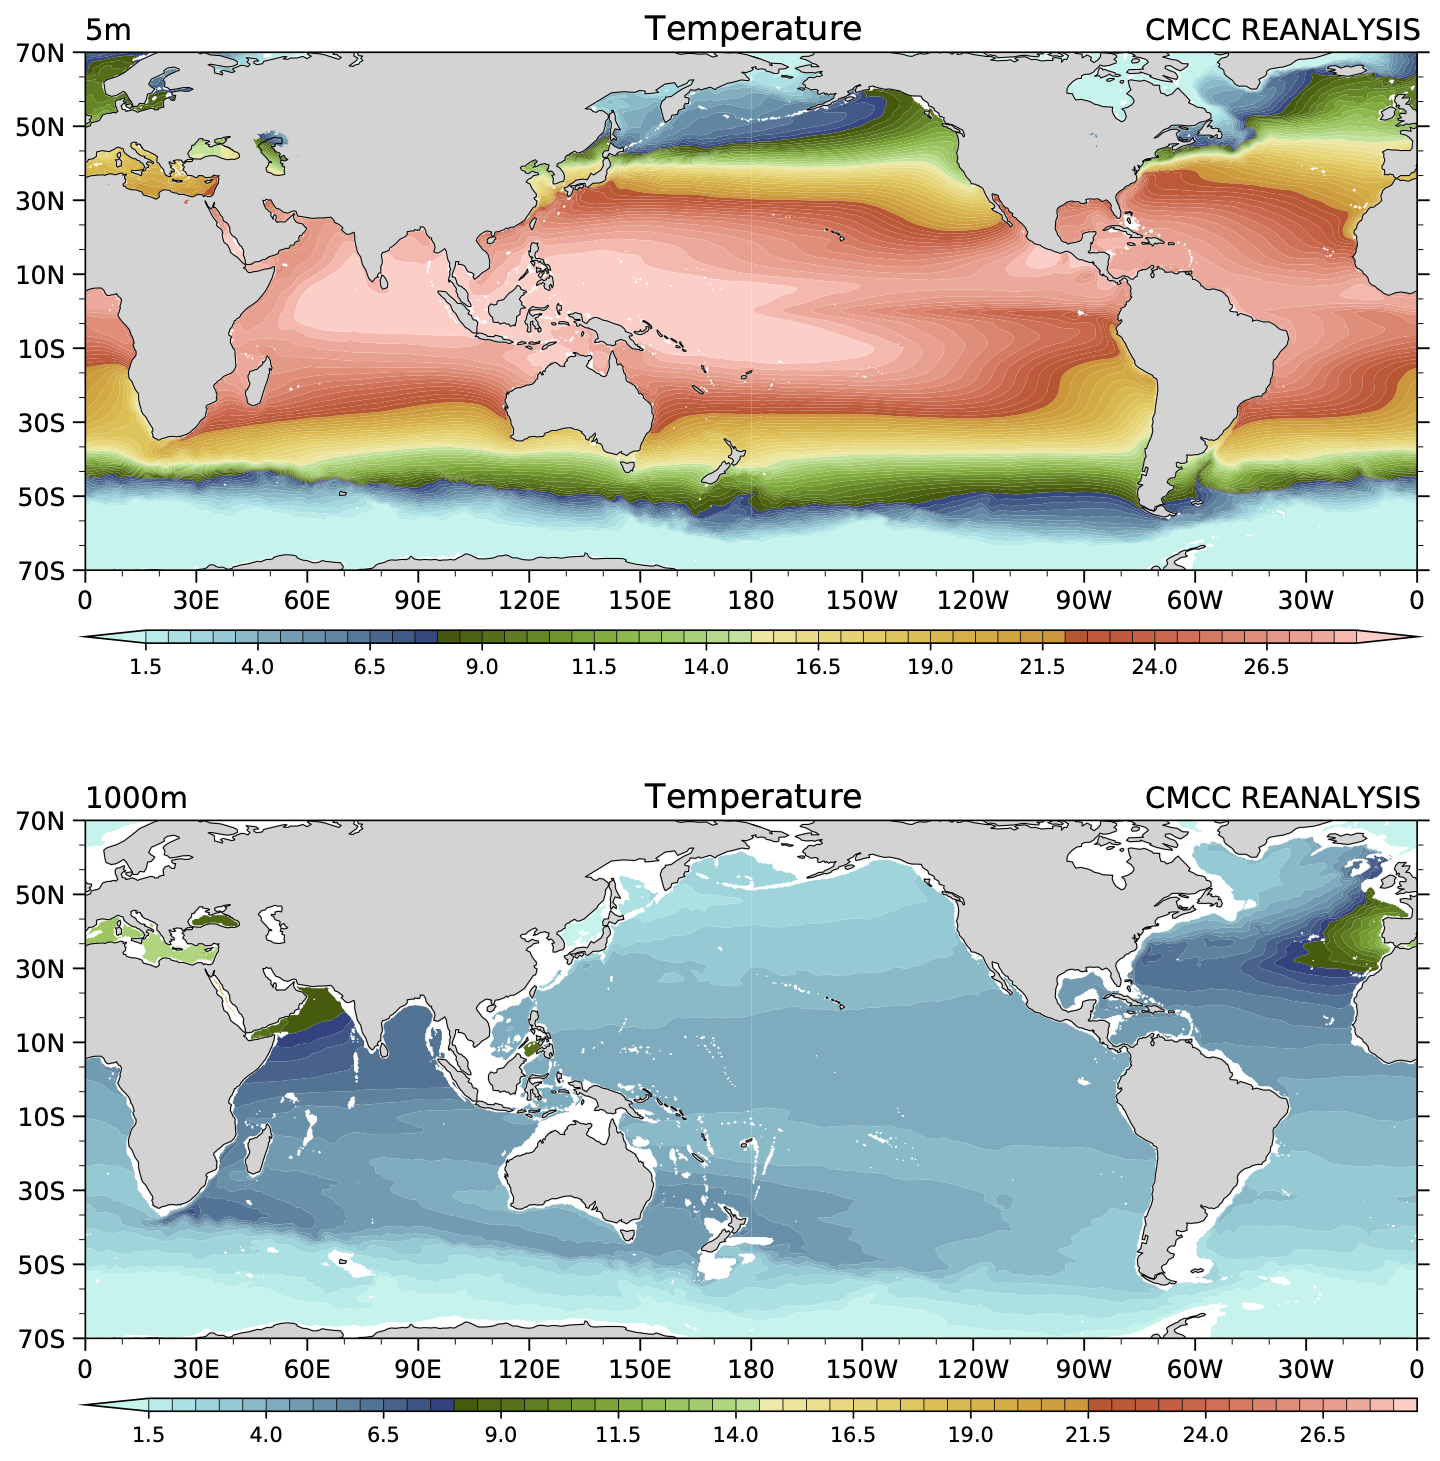
\includegraphics[width = .7 \textwidth]{figs/GD/Temp5-1000.png}
\caption{} \label{fig:}
\end{figure}

At the deeper depth pf 1000m (bottom panel) the ocean tends to be much
colder. We are using here the same scale to give a feeling of the
temperature drop. We can see that the general signature of the structure
that we have identified at the surface is still present, but there are
some interesting deviations.

In the North Atlantic the water is significantly warmer than the same
latitudes in the Pacific and it is easy to see that the origin of the
water is the Mediterranean that is contributing very warm waters to the
Atlantic via the Gibraltar Straits. The Mediterranean water penetrate
deeply into the Atlantic, basically up to the American coast.

\begin{figure}
\centering
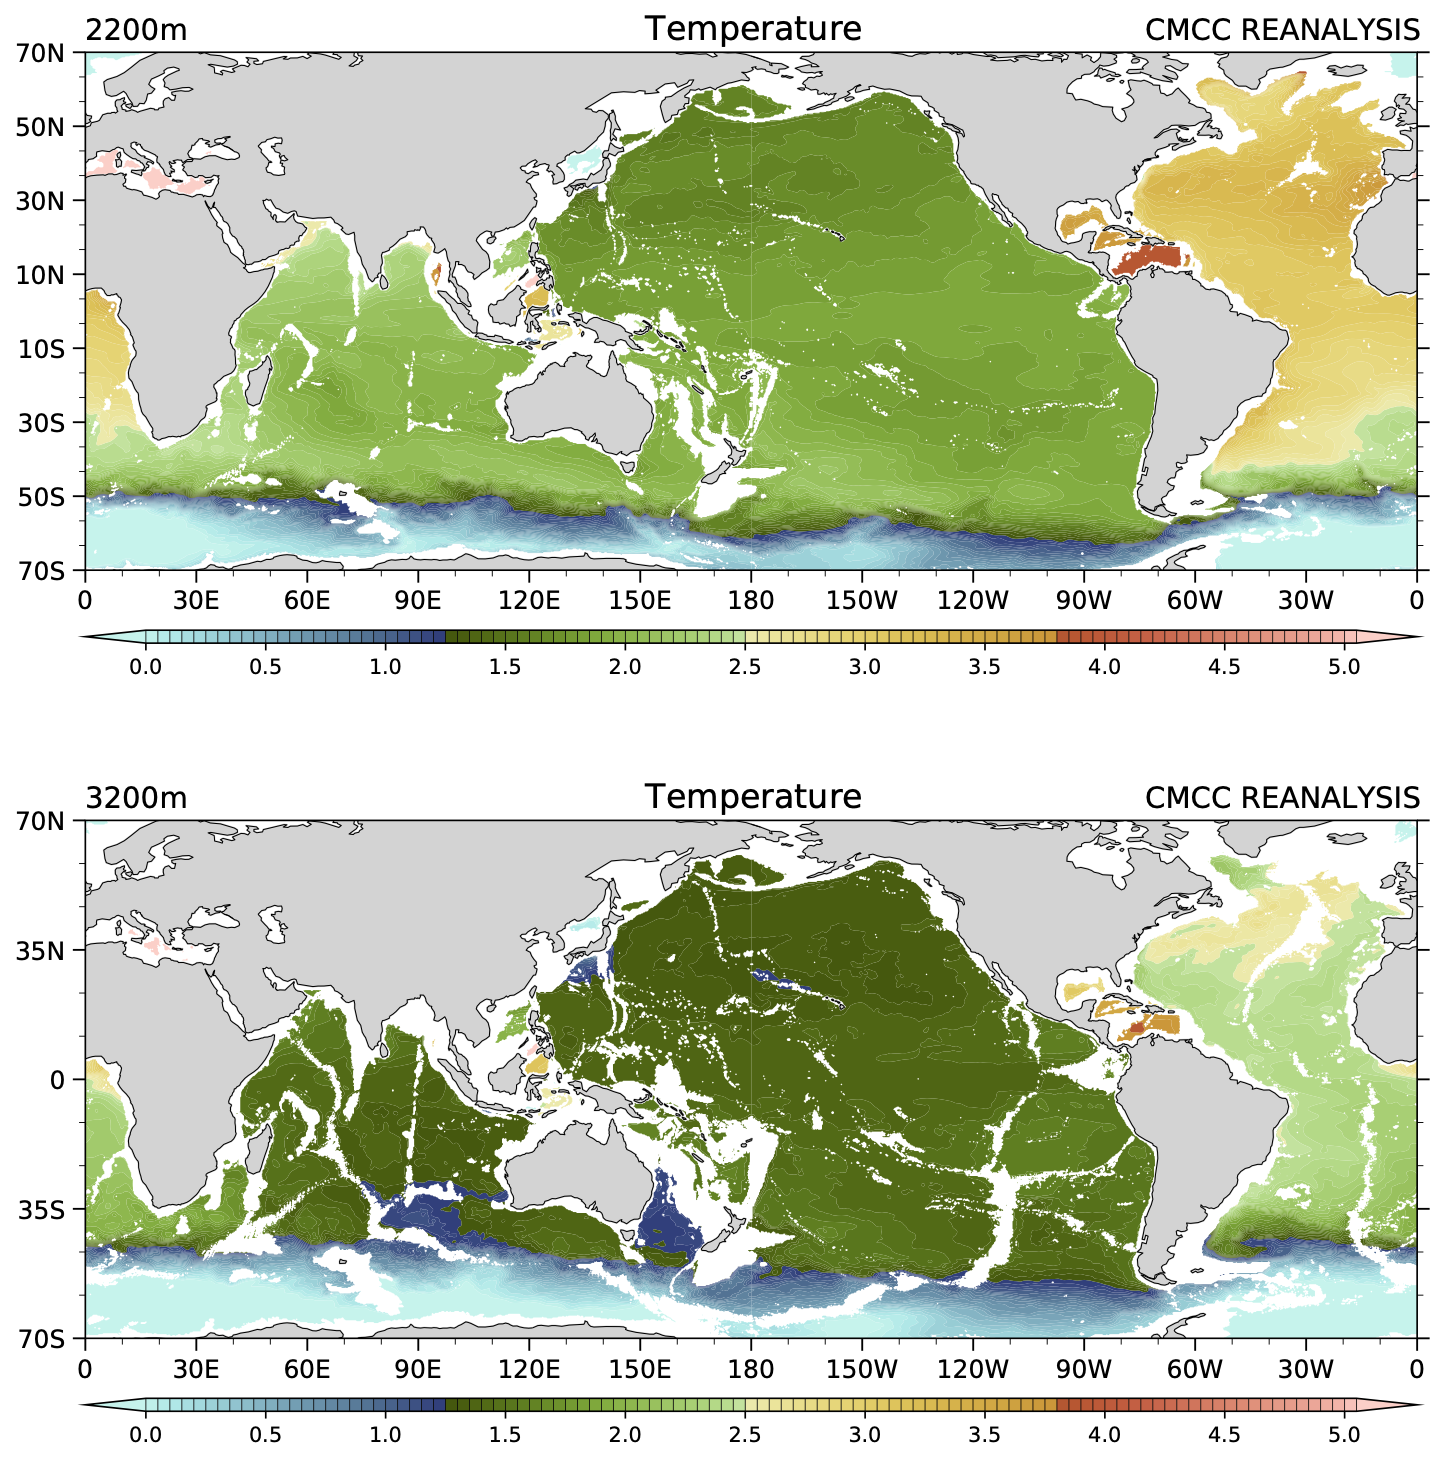
\includegraphics[width = .7 \textwidth]{figs/GD/Temp2200-3200.png}
\caption{} \label{fig:}
\end{figure}

Going even deeper (Fig. \texttt{fig:611}) we have to change drastically
the temperature scale. The typical temperature is now only a few
degrees. The Southern Ocean is very cold and the water is hovering
around 1.0 degree. The abyssal waters (Fig. \texttt{fig:612}) are
definitely colder and it is only the pressure that keeps them from
freezing when they get close to zero degrees. We cam also see
empirically how the average depth of the oceans is close to 4000 meter
as there are only limited areas that reach deeper depths. A precise,
quantitative calculation will yield the value of 4200? meters for the
average depth of the oceans.

\begin{figure}
\centering
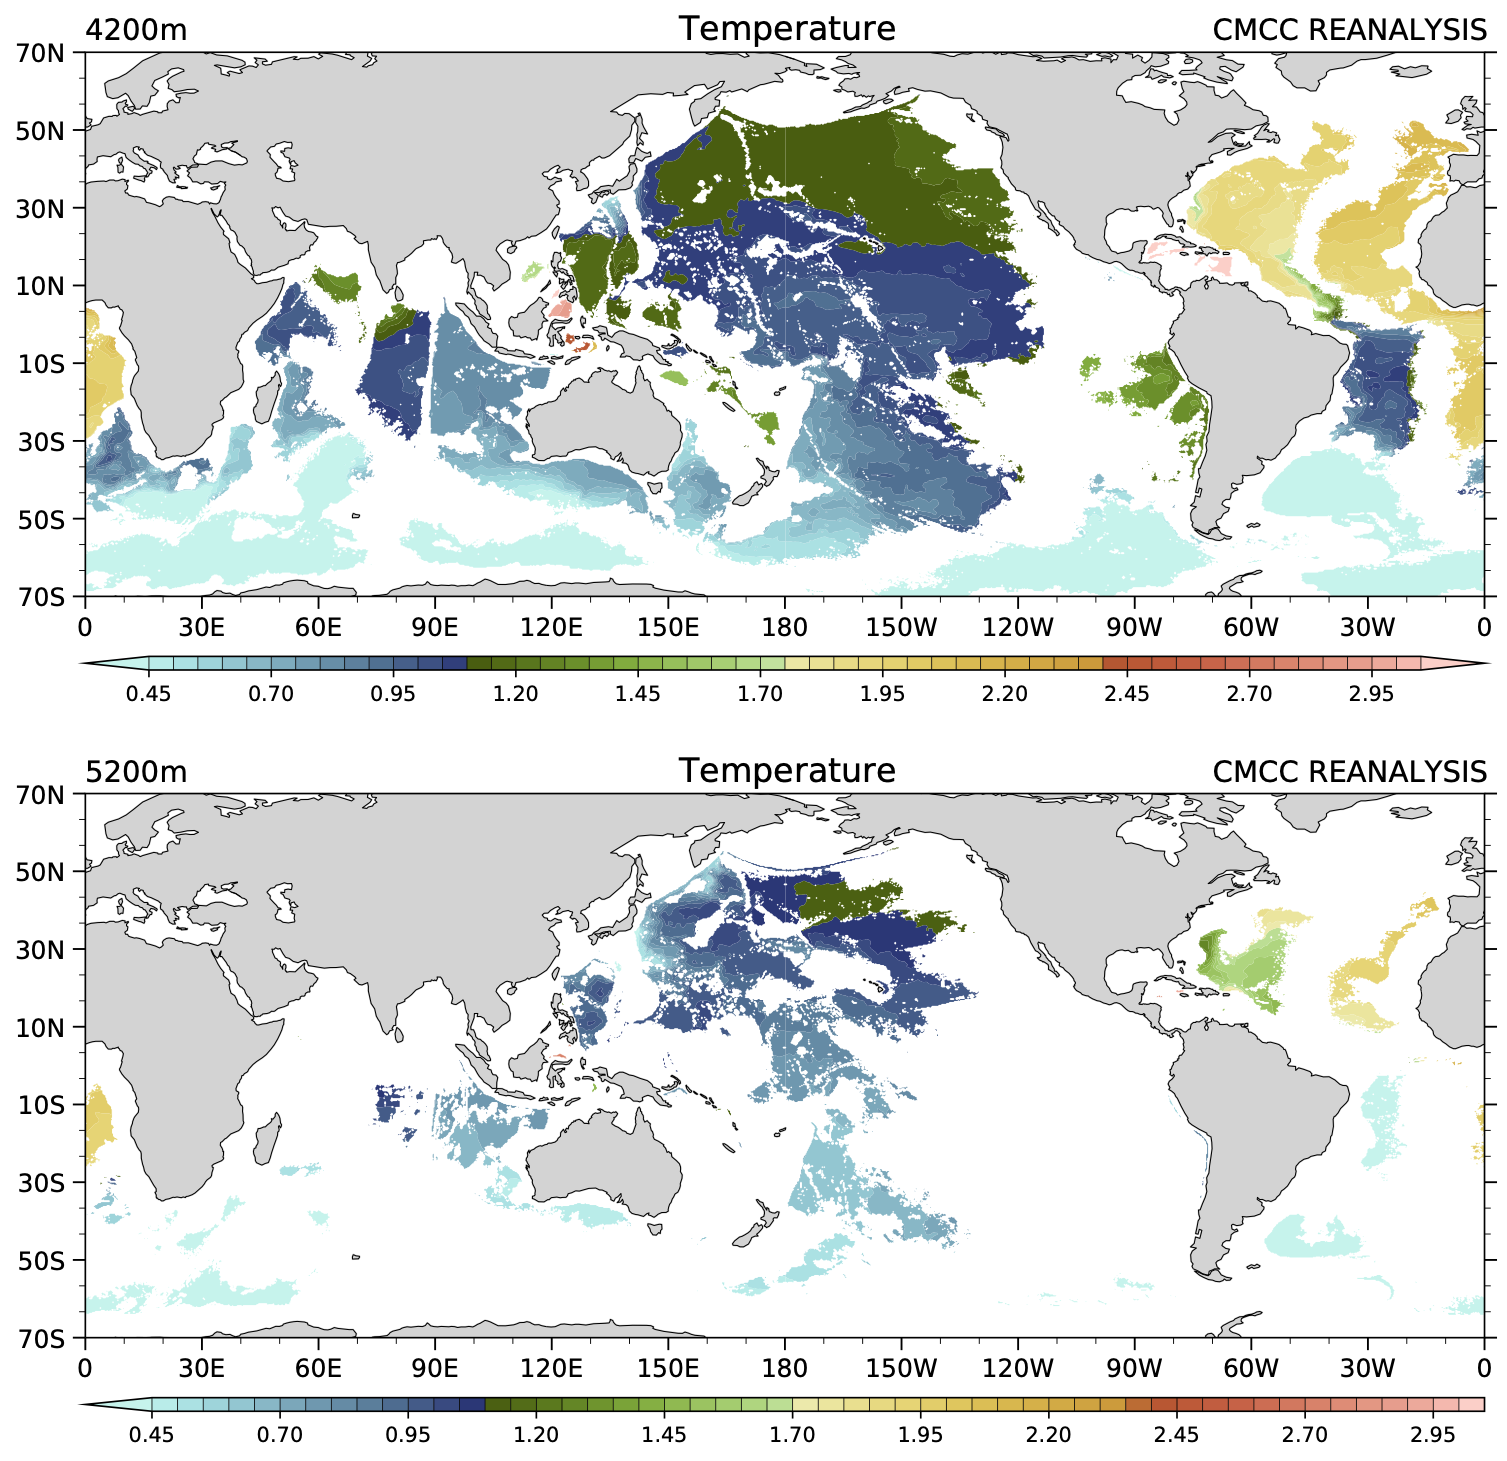
\includegraphics[width = .7 \textwidth]{figs/GD/Temp4200-5200.png}
\caption{} \label{fig:}
\end{figure}

A qualitative look at this pictures already gives the impression of the
diversity among the various Oceans. We can guess that the dynamics of
the Souther Ocean, colder and basically unimpeded by continental
boundaries in a single circle around the South Pole is probably going to
be different from all others. By the same token, the warmer Atlantic,
deeply affected by the Mediterranean inflow is going to show different
characteristics from the Northern Pacific, colder and larger.

A closer look will reveal further differences between the mid-latitude
oceans and the tropical oceans. Looking at the North Atlantic (Fig.
\texttt{fig:613}) we notice the strong gradients along the North
American Coast that persists up to 1000m. Strong temperature gradients
are presumably to be connected to the existence of currents, but we will
need to check the density, depending on the salinity later, to be really
sure. Anyway, this picture is giving a strong indication of the
existence of something remarkable and intense along the western boundary
of the Atlantic ocean.

\begin{figure}
\centering
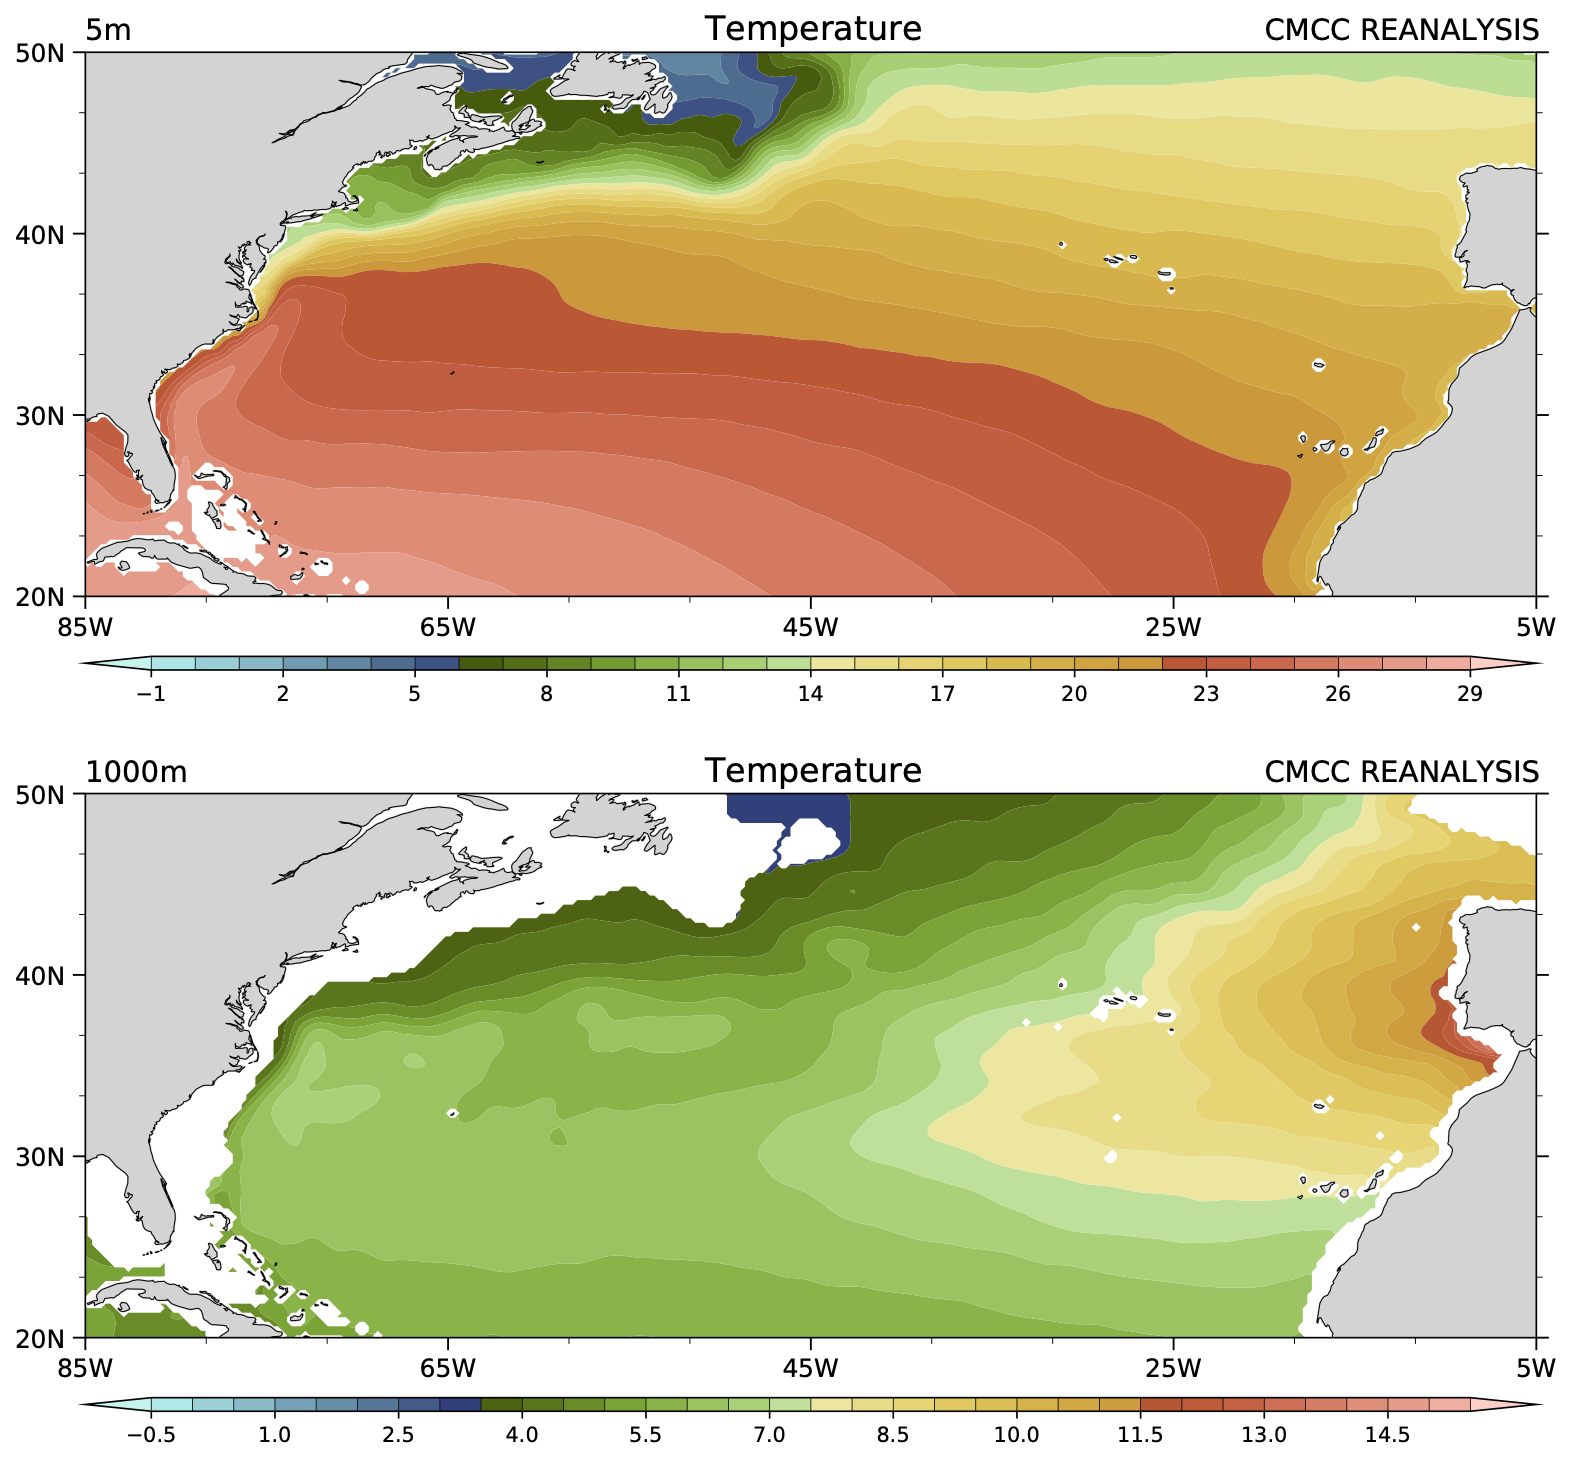
\includegraphics[width = .7 \textwidth]{figs/GD/Gulf1000.png}
\caption{} \label{fig:}
\end{figure}

Warm waters are protruding from the Gibraltar Straits into the Atlantic.
They are not very visible at the surface, but they are remarkably well
clear at depth, for instance the 100m shown here. The warm water is
sinking, indicating that its density is higher than the surrounding
water, notwithstanding the higher temperature.

The North Pacific shows something similar along the Japan coast and
therefore we can start to suspect that this has to do with the presence
of the continental boundary. Without the Mediterranean, the vertical
structure is more uniform and we can notice a progressive cooling of the
water.

\begin{figure}
\centering
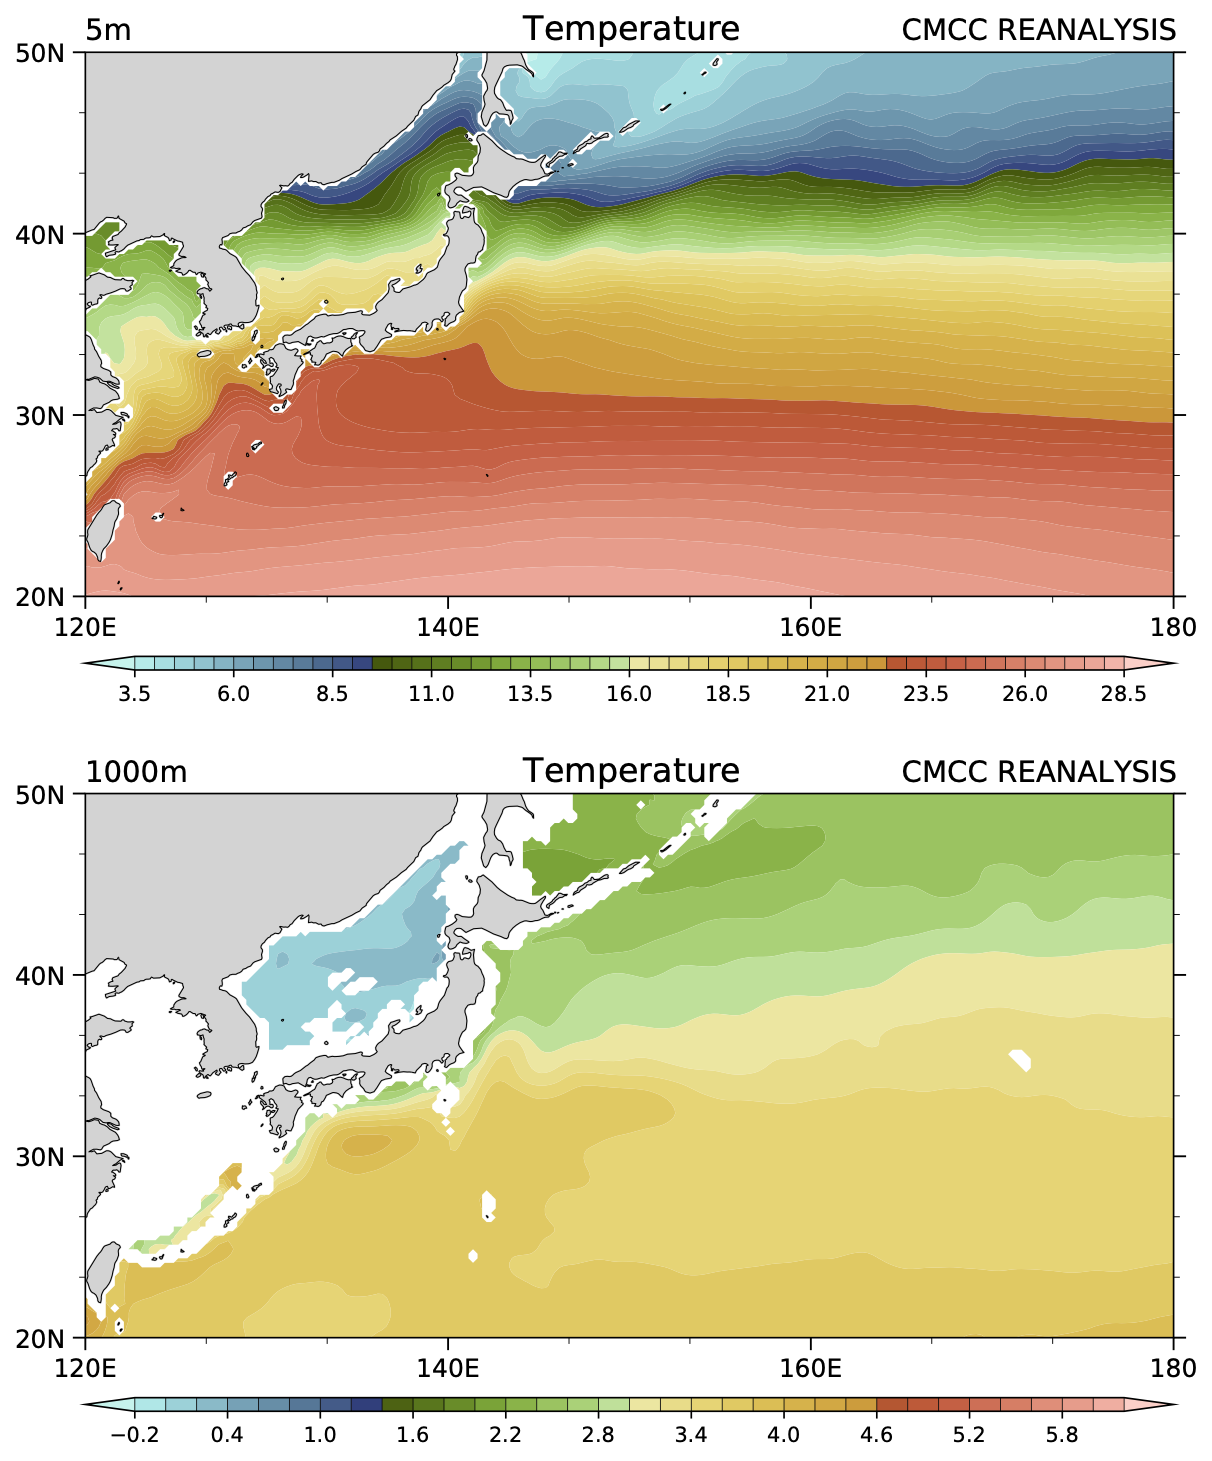
\includegraphics[width = .7 \textwidth]{figs/GD/Kur1000.png}
\caption{} \label{fig:}
\end{figure}

The preliminary analysis is giving us hints of a strong vertical
structure of the oceans, soit may be useful to look at the vertical
distribution somewhat more in detail. Fig. \texttt{fig:6100} shows a
North-South section along the longitude of 25W, roughly in the middle of
the Atlantic Ocean. The bottom panel reaches to 5000m, it is very
evident the strong stratification of the ocean. An area of high
variation, where the temperature cools down quickly, appears around
800-1000m, more prominent in the Southern Hemisphere, below that the
ocean is more uniform and very cold. This sharp transition region is
called \emph{thermocline}.

It is interesting to note how layers of water of the same temperature
can reach the surface, as it can be seen from the picture and, in more
detail, from the top panel. The layers connect even considerable depths,
like is the case for the very cold water around 2-4 C that rises from
the bottom of the Southern Ocean surfacing into the Antarctic region.

\begin{figure}
\centering
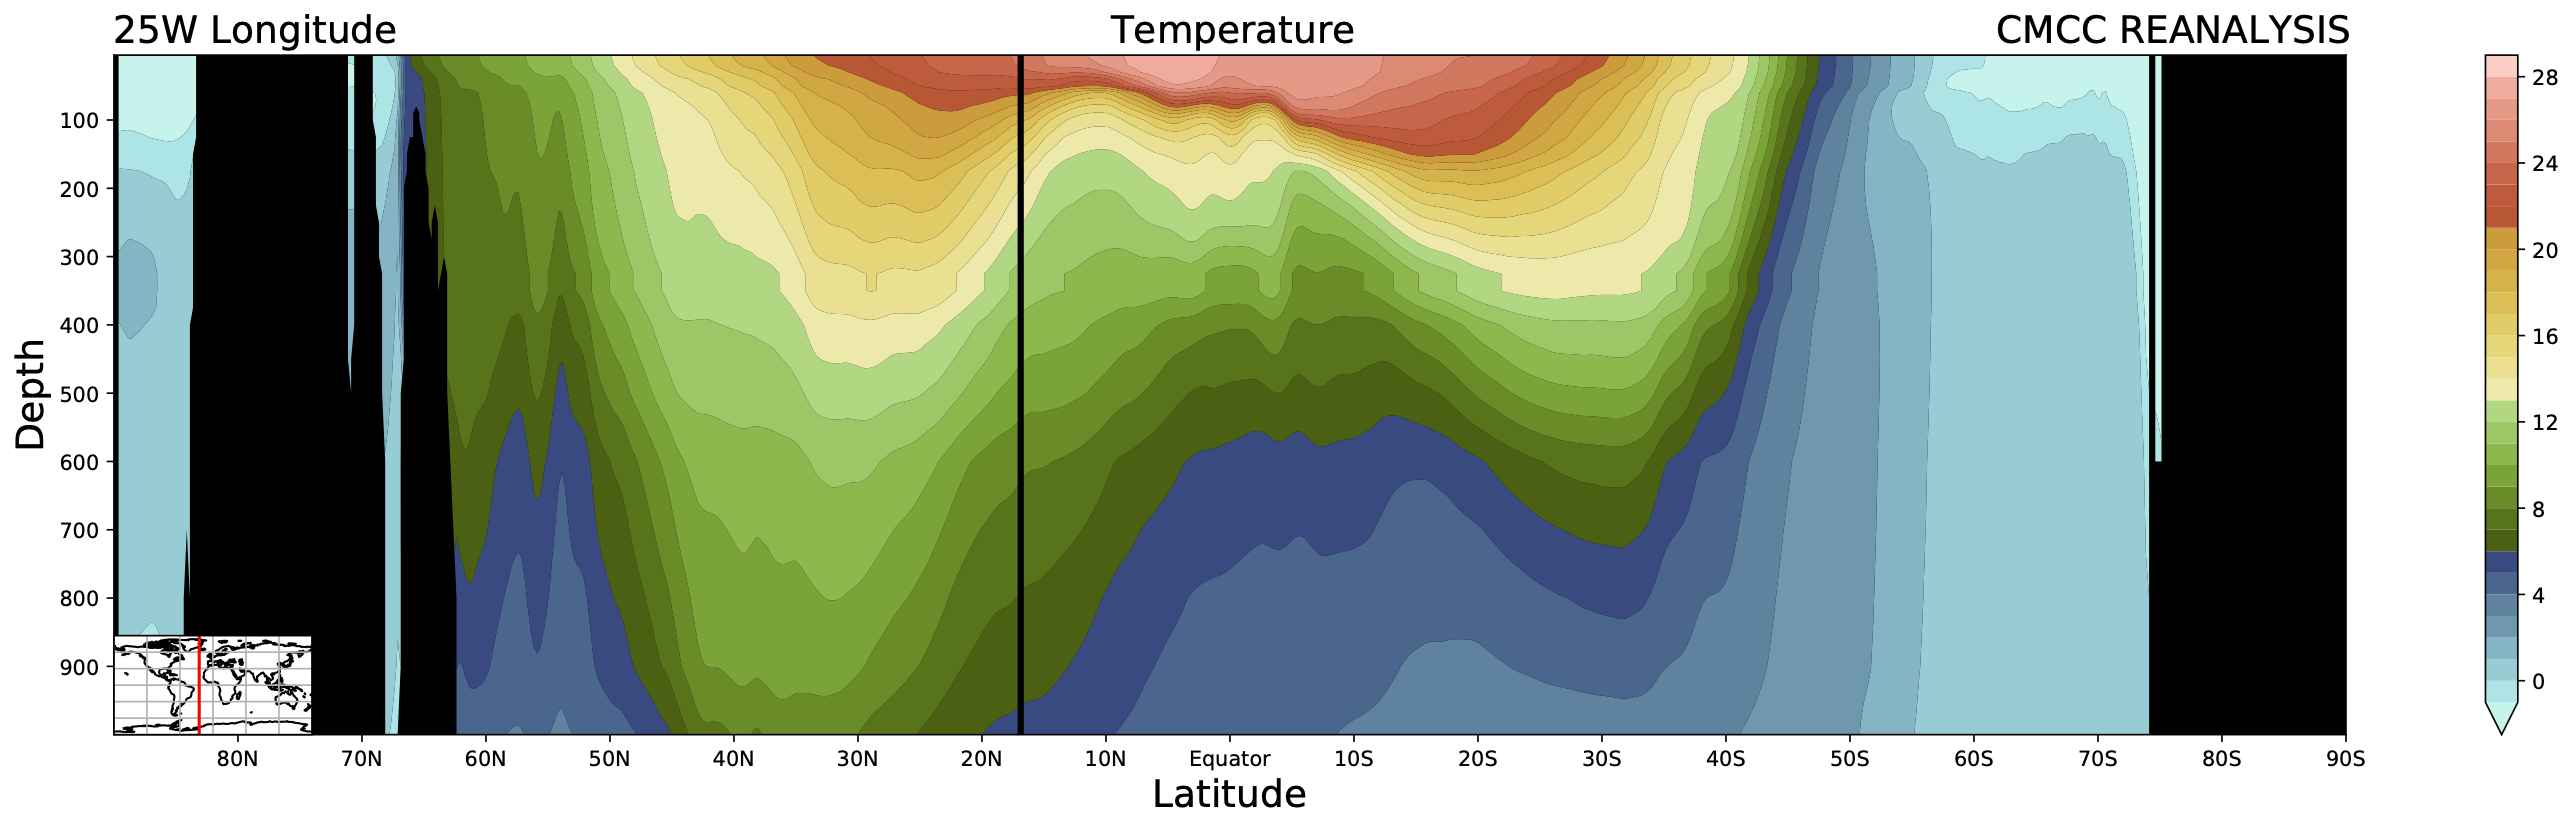
\includegraphics[width = .7 \textwidth]{figs/GD/Sect25W1000.png}
\caption{} \label{fig:}
\end{figure}

\begin{figure}
\centering
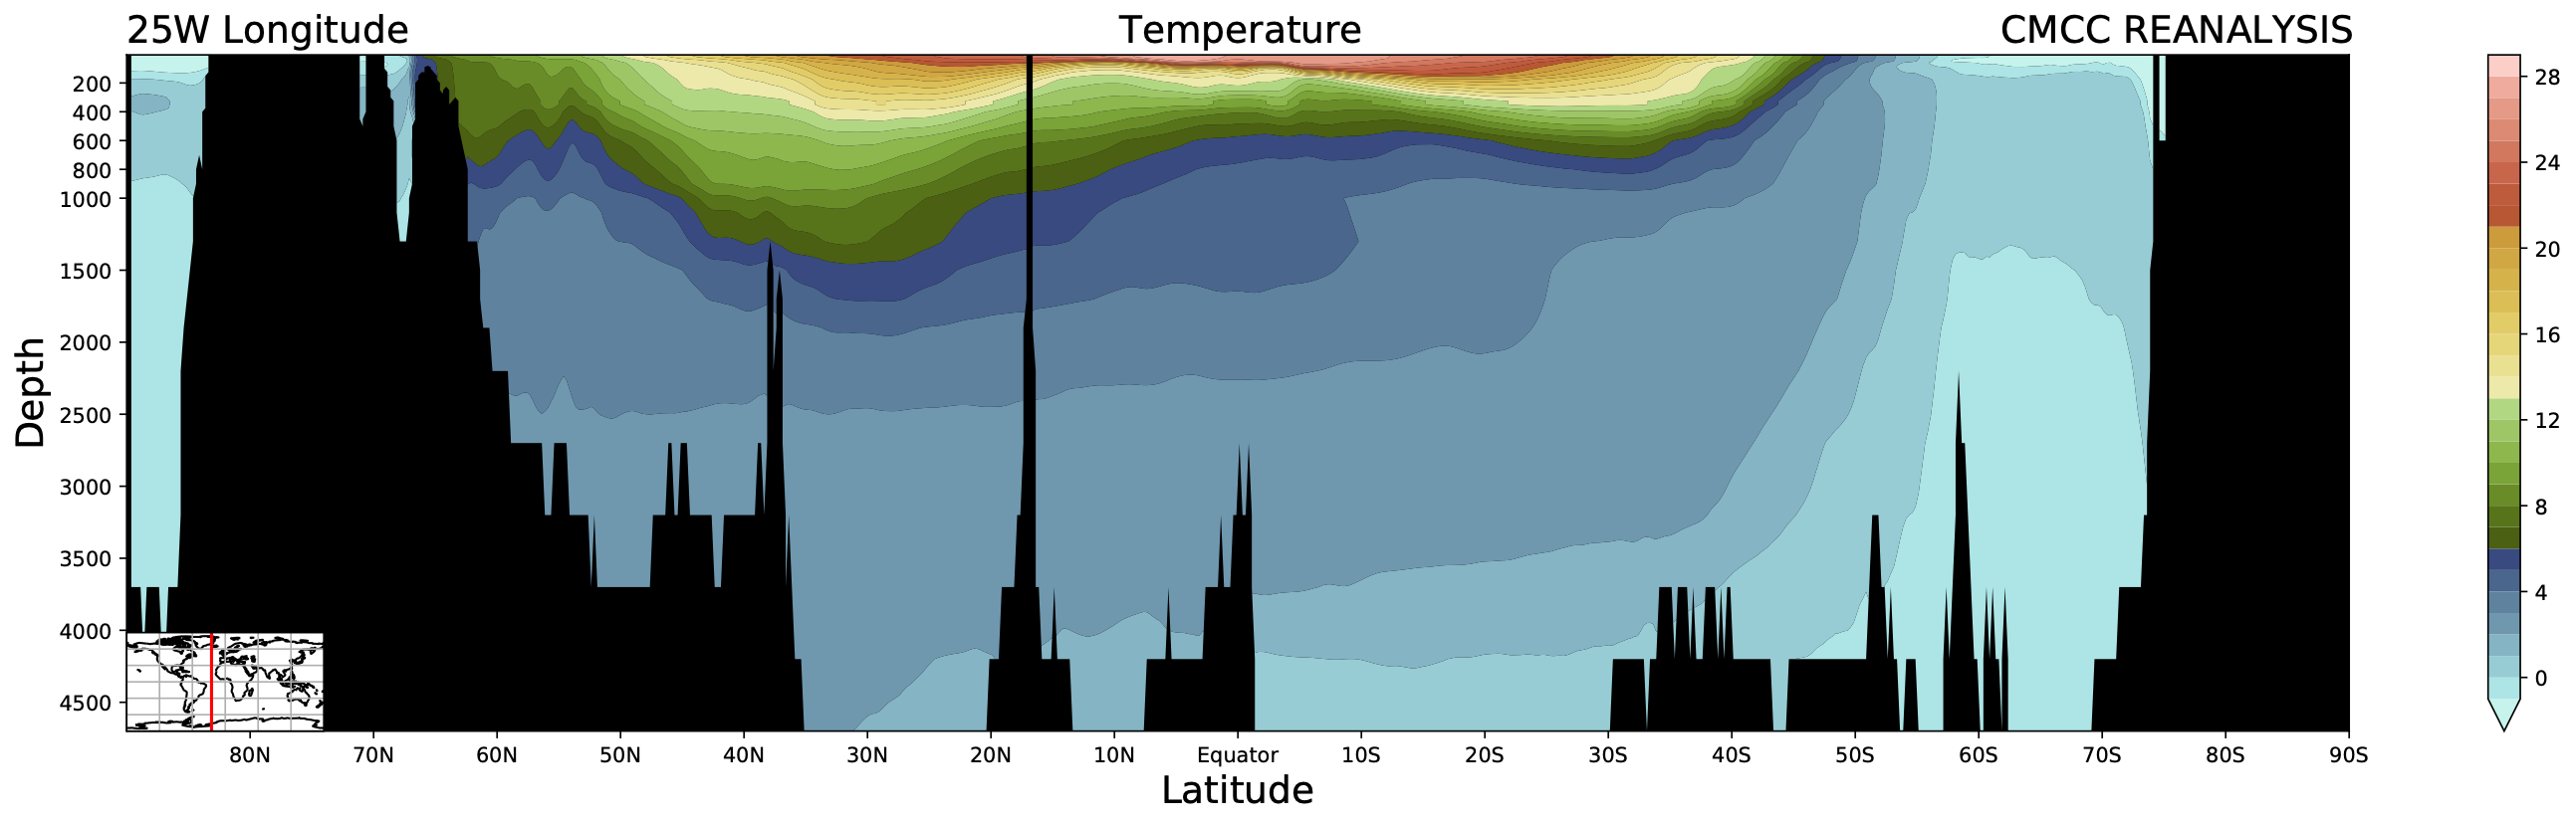
\includegraphics[width = .7 \textwidth]{figs/GD/Sect25W5000.png}
\caption{} \label{fig:}
\end{figure}

The signature of the Mediterranean outflow can be seen in the asymmetry
between the hemispheres that pushes relatively warmer water down in the
Northern Atlantic relatively to the Southern part of the ocean.

\begin{figure}
\centering
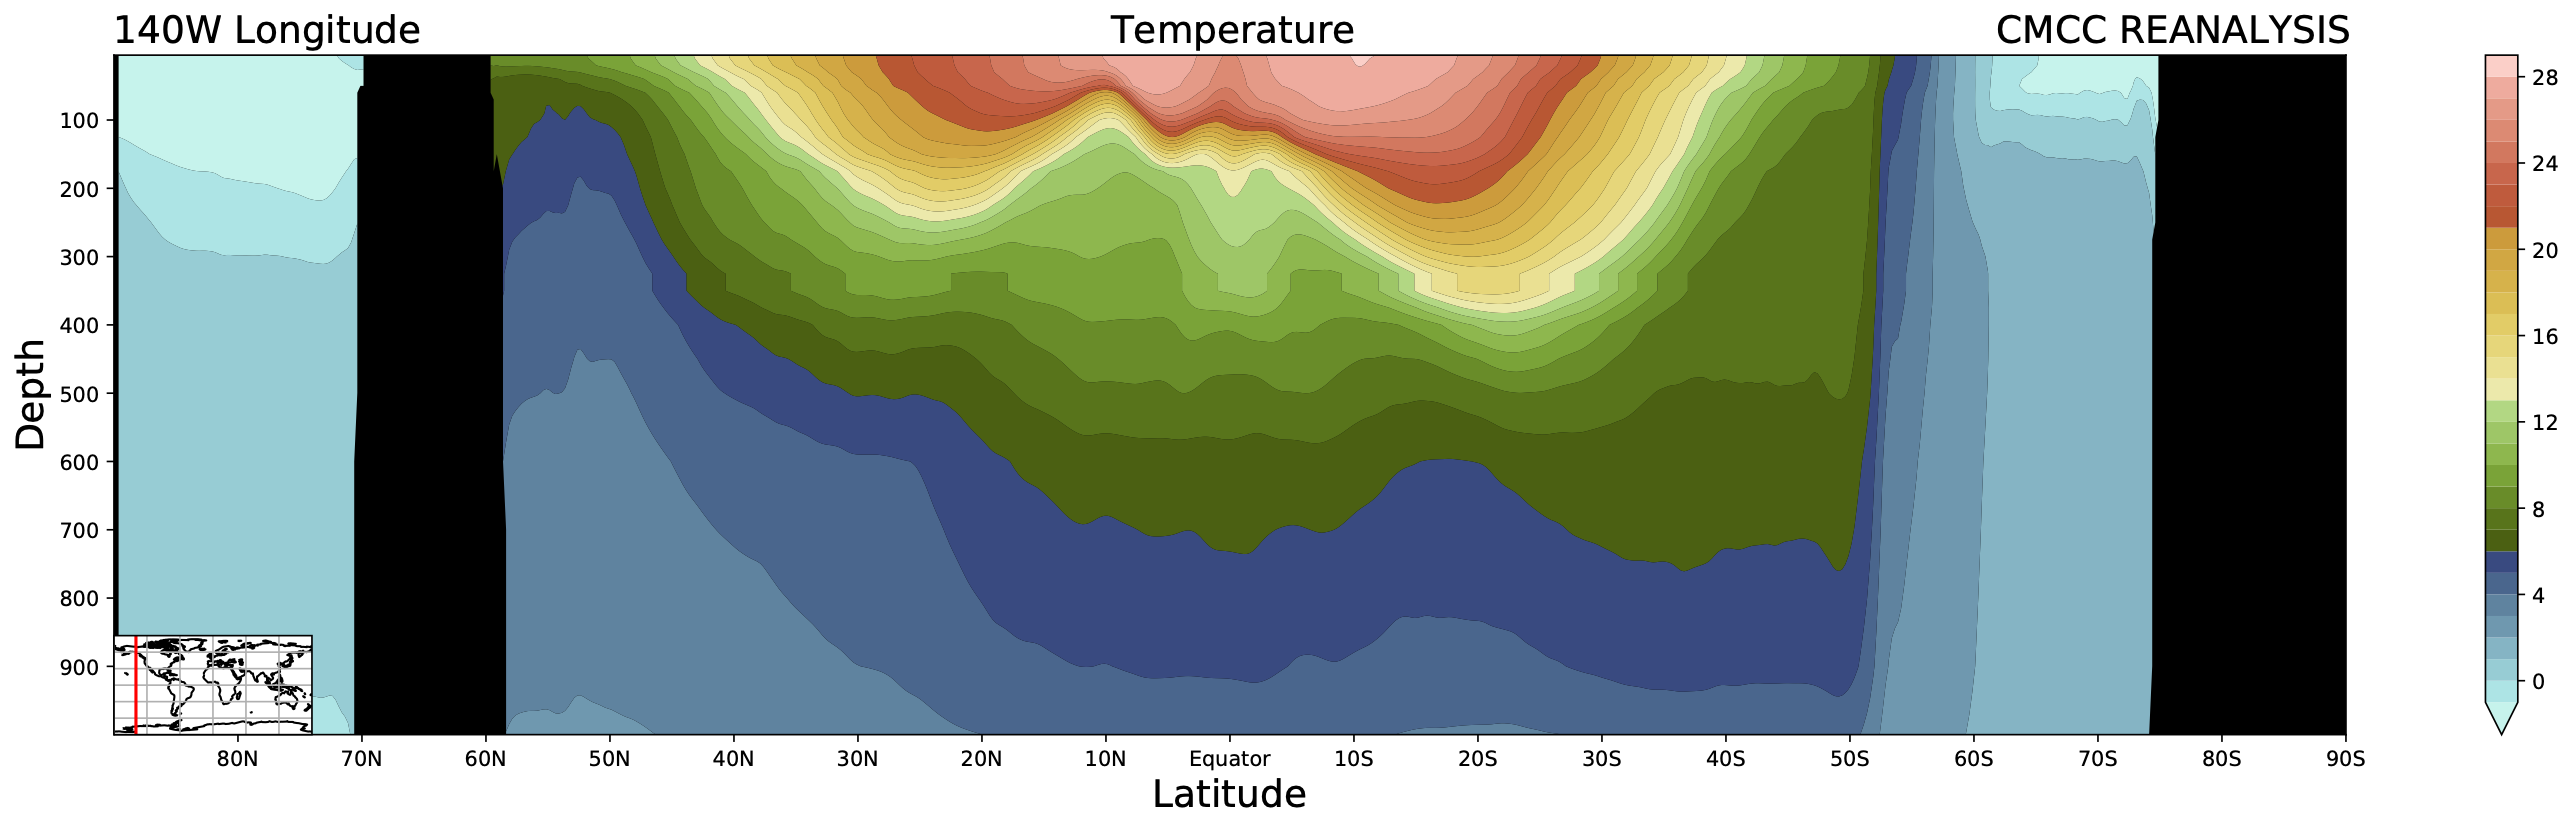
\includegraphics[width = .7 \textwidth]{figs/GD/Sect140W1000.png}
\caption{As in Fig. \texttt{fig:6100} but for 140W longitude}
\end{figure}

\begin{figure}
\centering
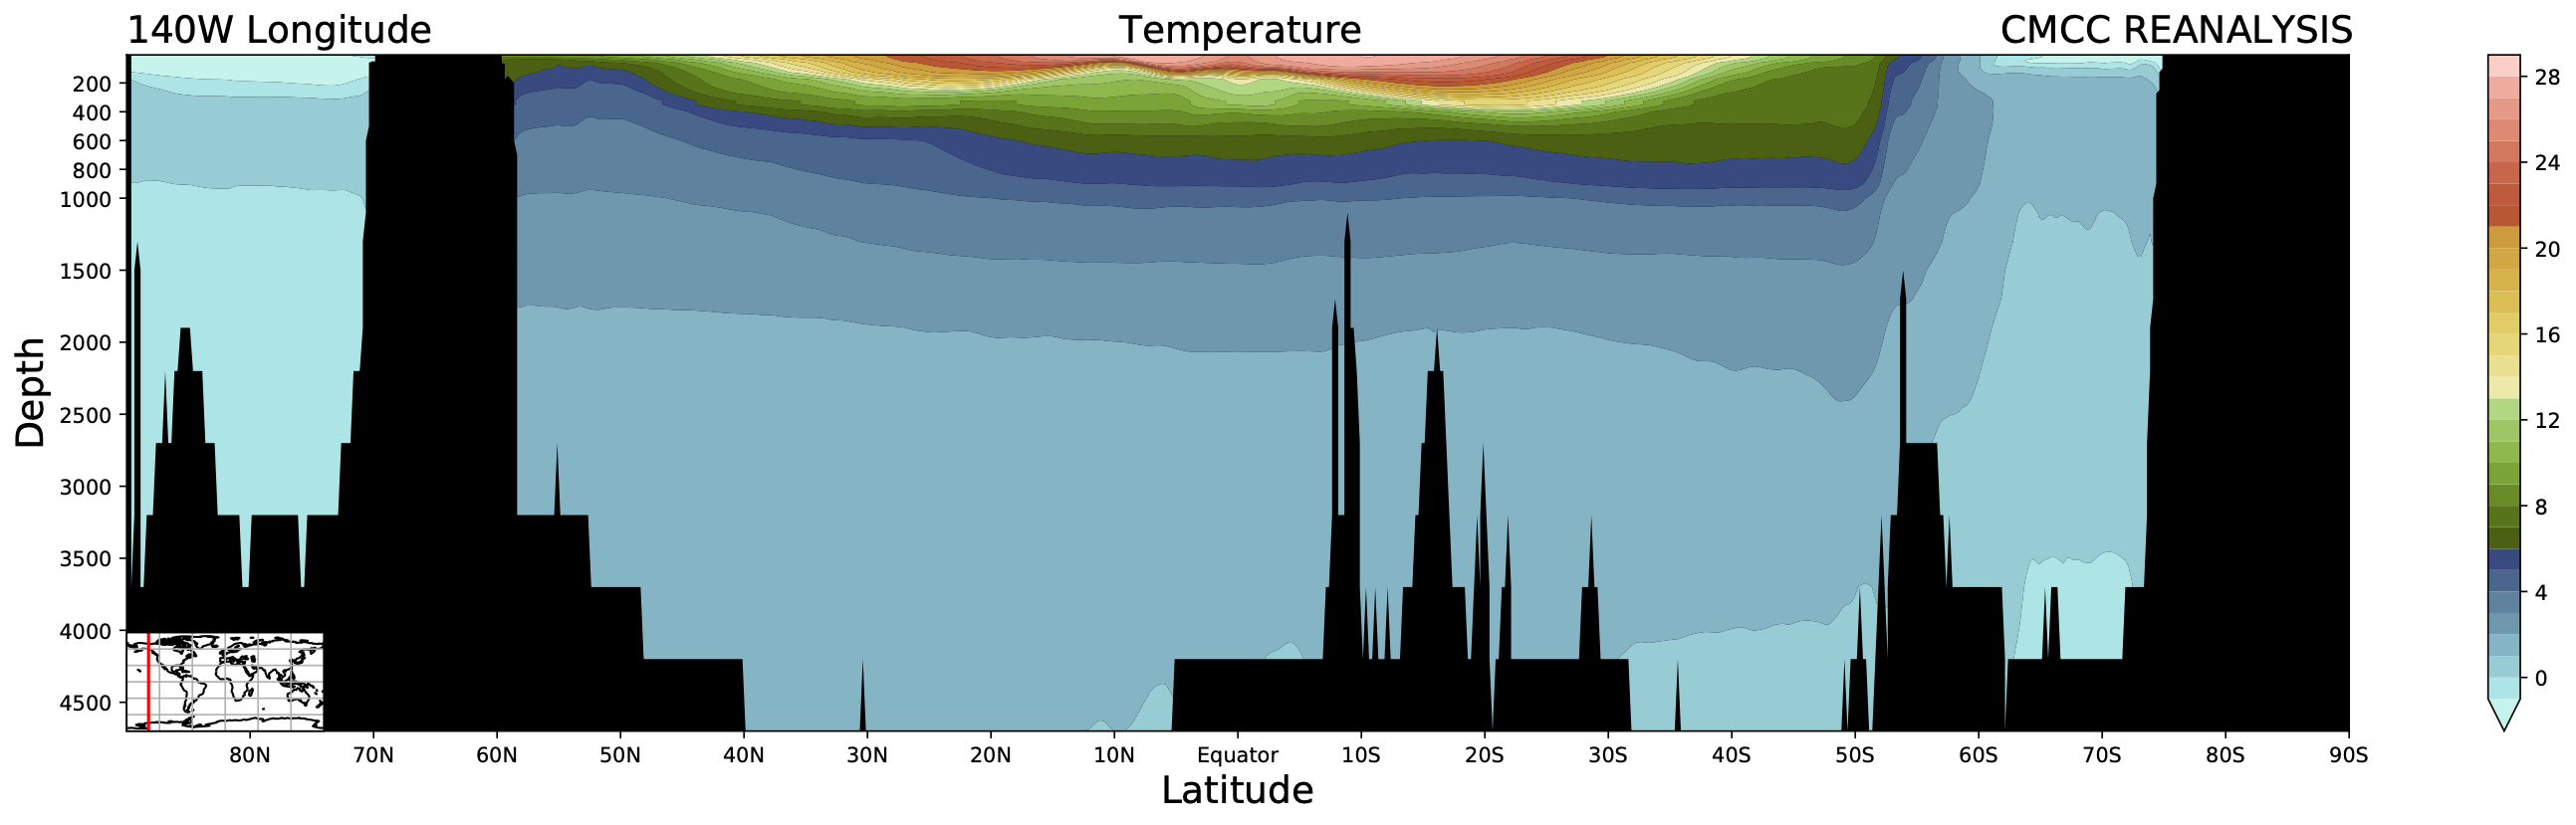
\includegraphics[width = .7 \textwidth]{figs/GD/Sect140W5000.png}
\caption{As in Fig. \texttt{fig:6100a} but for 140W longitude}
\end{figure}

Looking at a similar section in the middle of the Pacific Ocean at 140W
longitude we see a different situation. The relatively warm waters are
confined to a much shallower region confined to the subtropics. In this
basin is also more noticeable a phenomenon that was present also in the
Atlantic, namely the raising of cold water in the equatorial region that
is the signature of the cold tongue of equatorial water that lays in the
equatorial Pacific Ocean. Also in this case the layers of different
temperature reach the surface at different latitudes. Especially in the
Southern Hemisphere is possible to see the deep, cold abyssal water
connecting with the surface at very high southern latitudes.

\begin{figure}
\centering
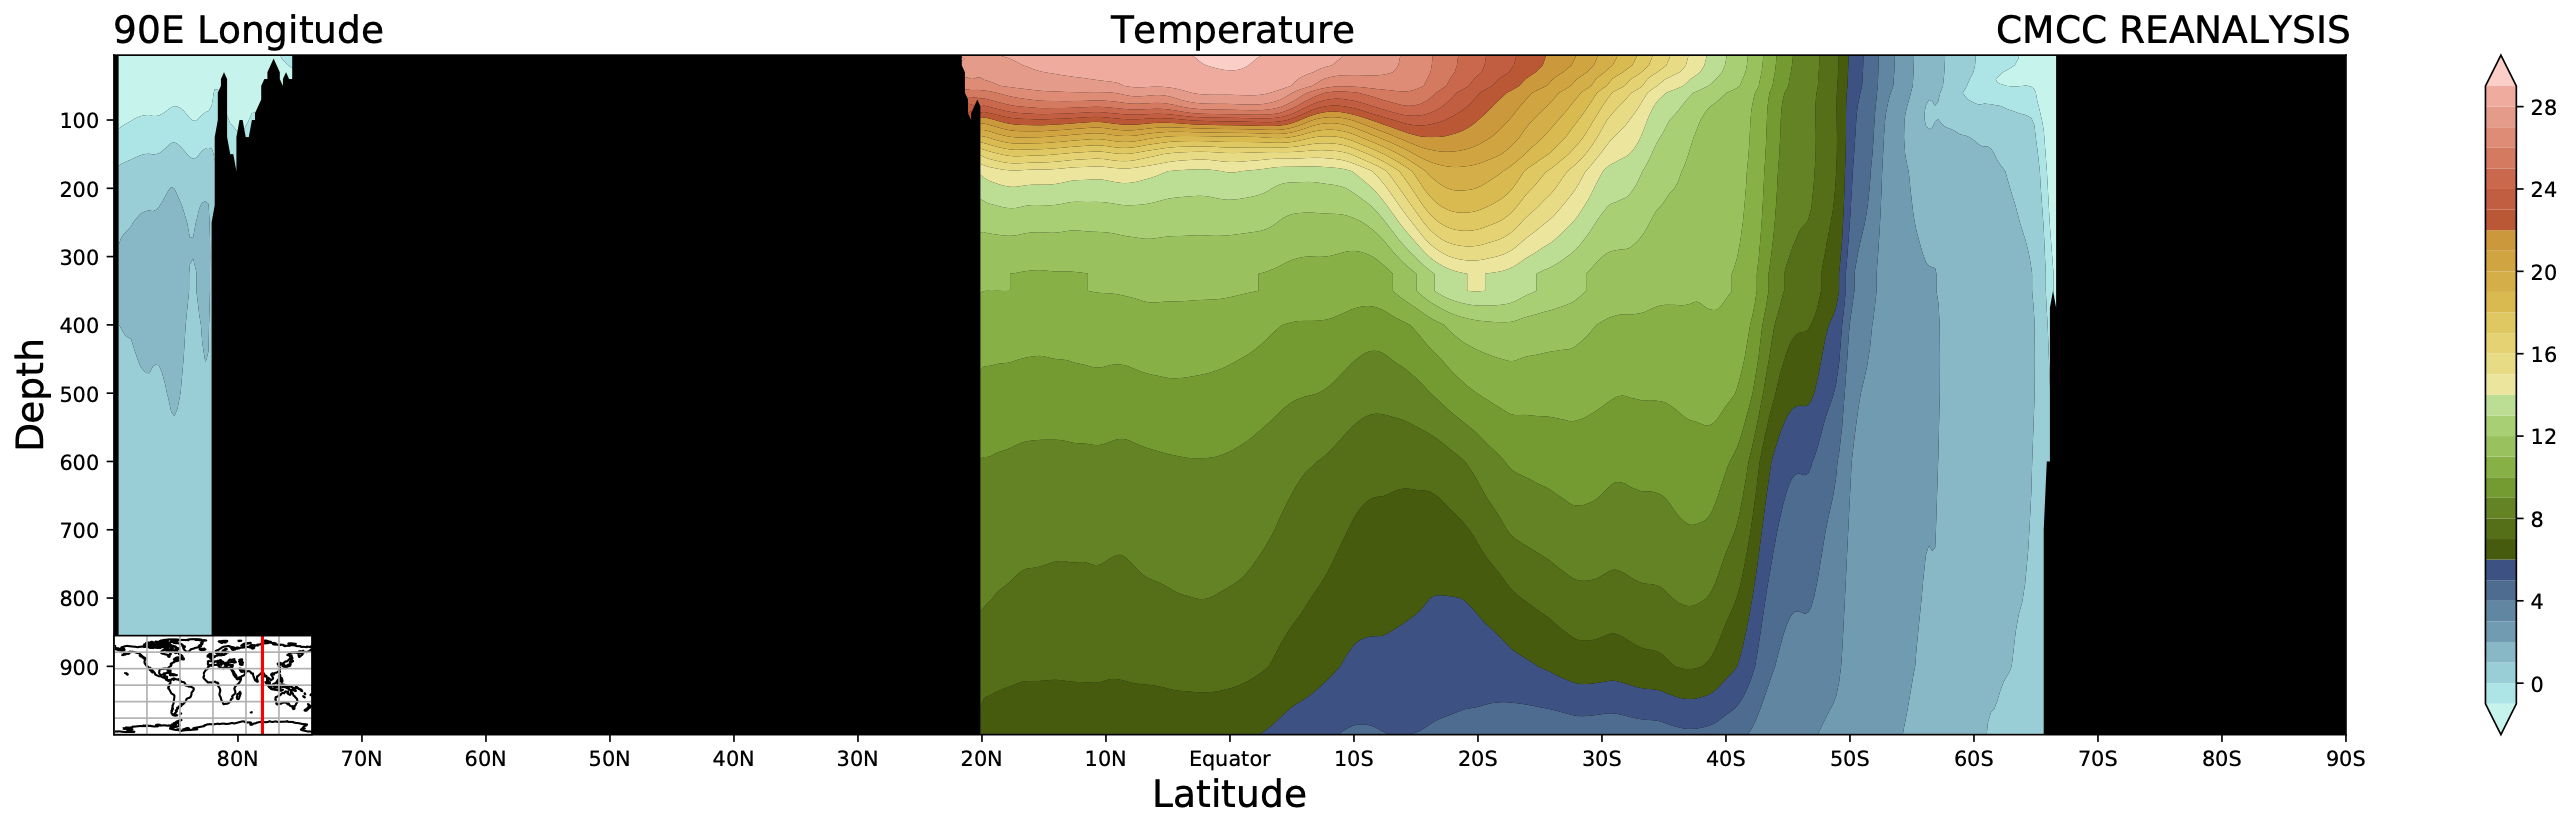
\includegraphics[width = .7 \textwidth]{figs/GD/Sect90E1000.png}
\caption{As in Fig. \texttt{fig:6100} but for 90E longitude}
\end{figure}

\begin{figure}
\centering
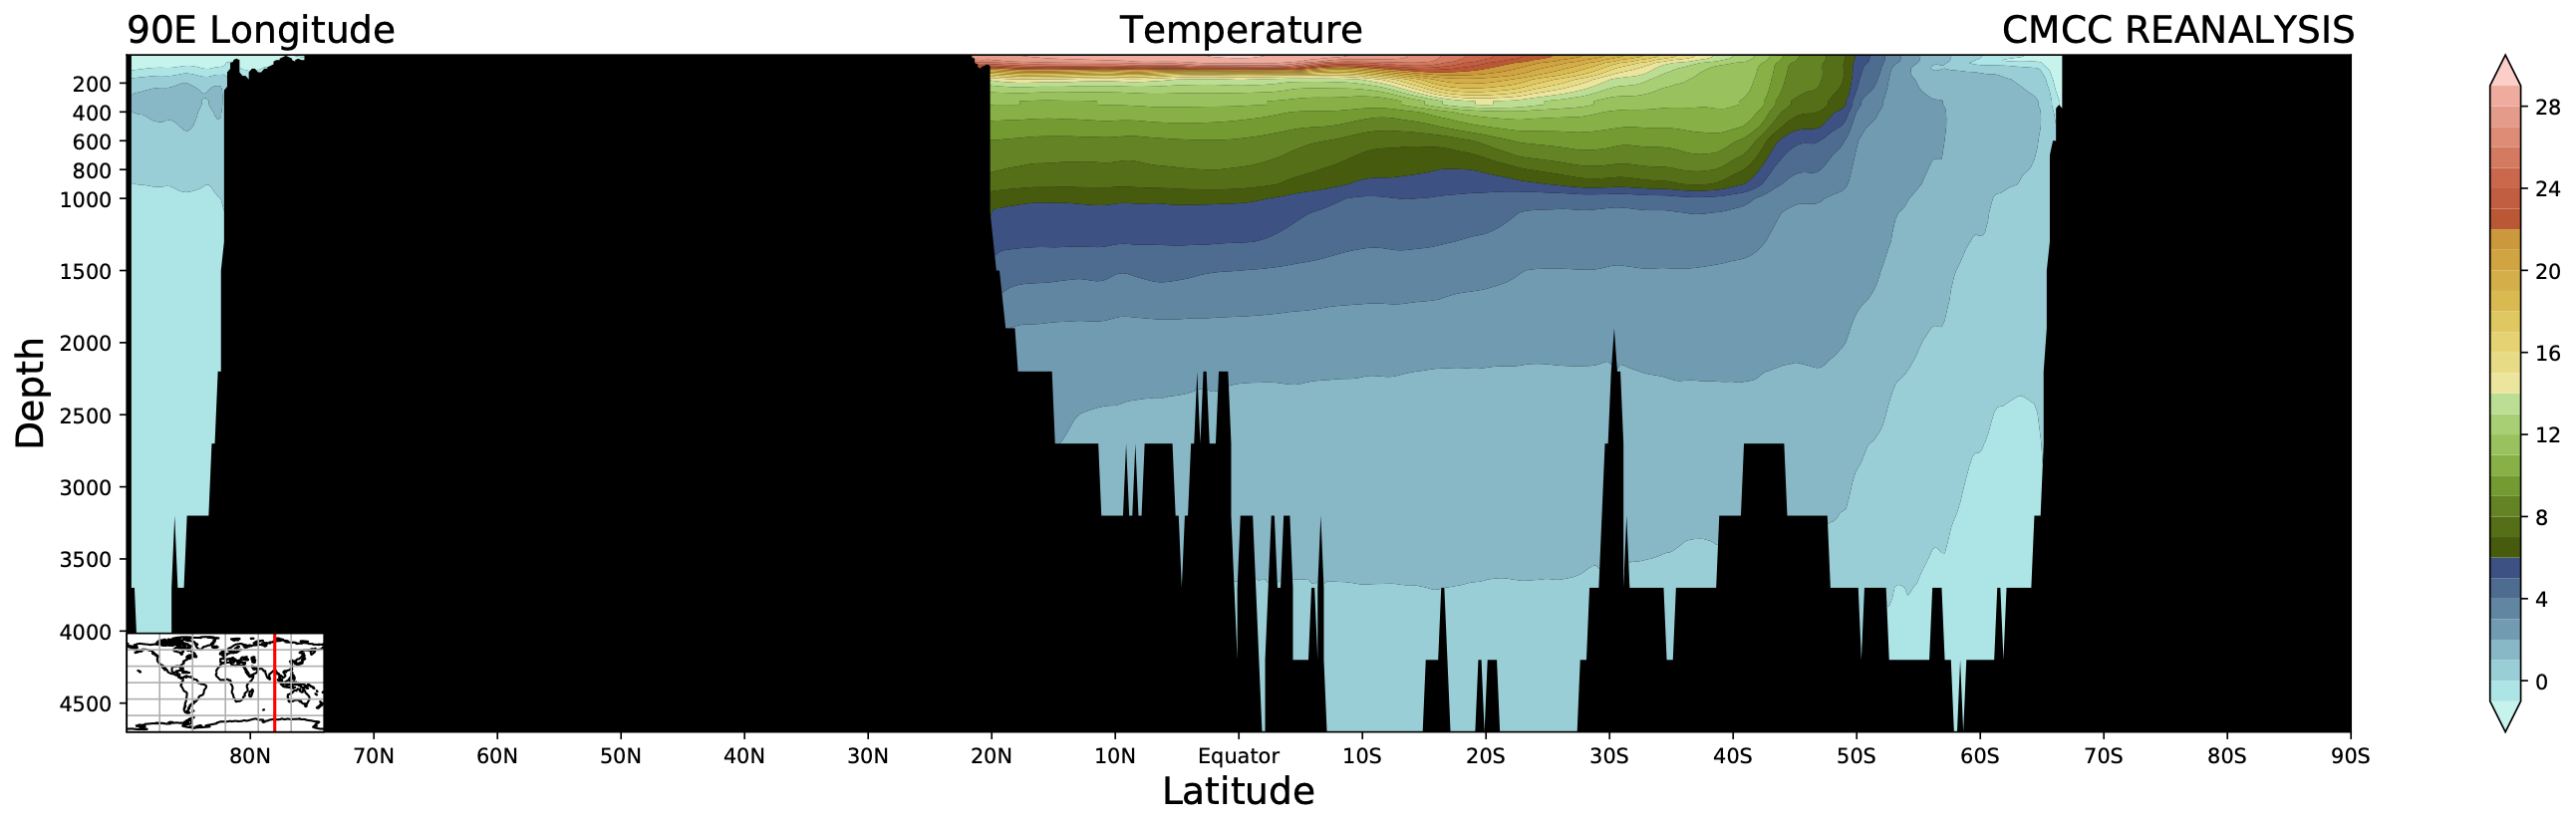
\includegraphics[width = .7 \textwidth]{figs/GD/Sect90E5000.png}
\caption{As in Fig. \texttt{fig:6100a} but for 90E longitude}
\end{figure}

The Indian Ocean (Fig. \texttt{fig:6102}) shown here as a section
cutting essentially through the Bay of Bengal, shows a similar strong
stratification, but there are only weak signs of an equatorial upwelling
of cold water.

\begin{figure}
\centering
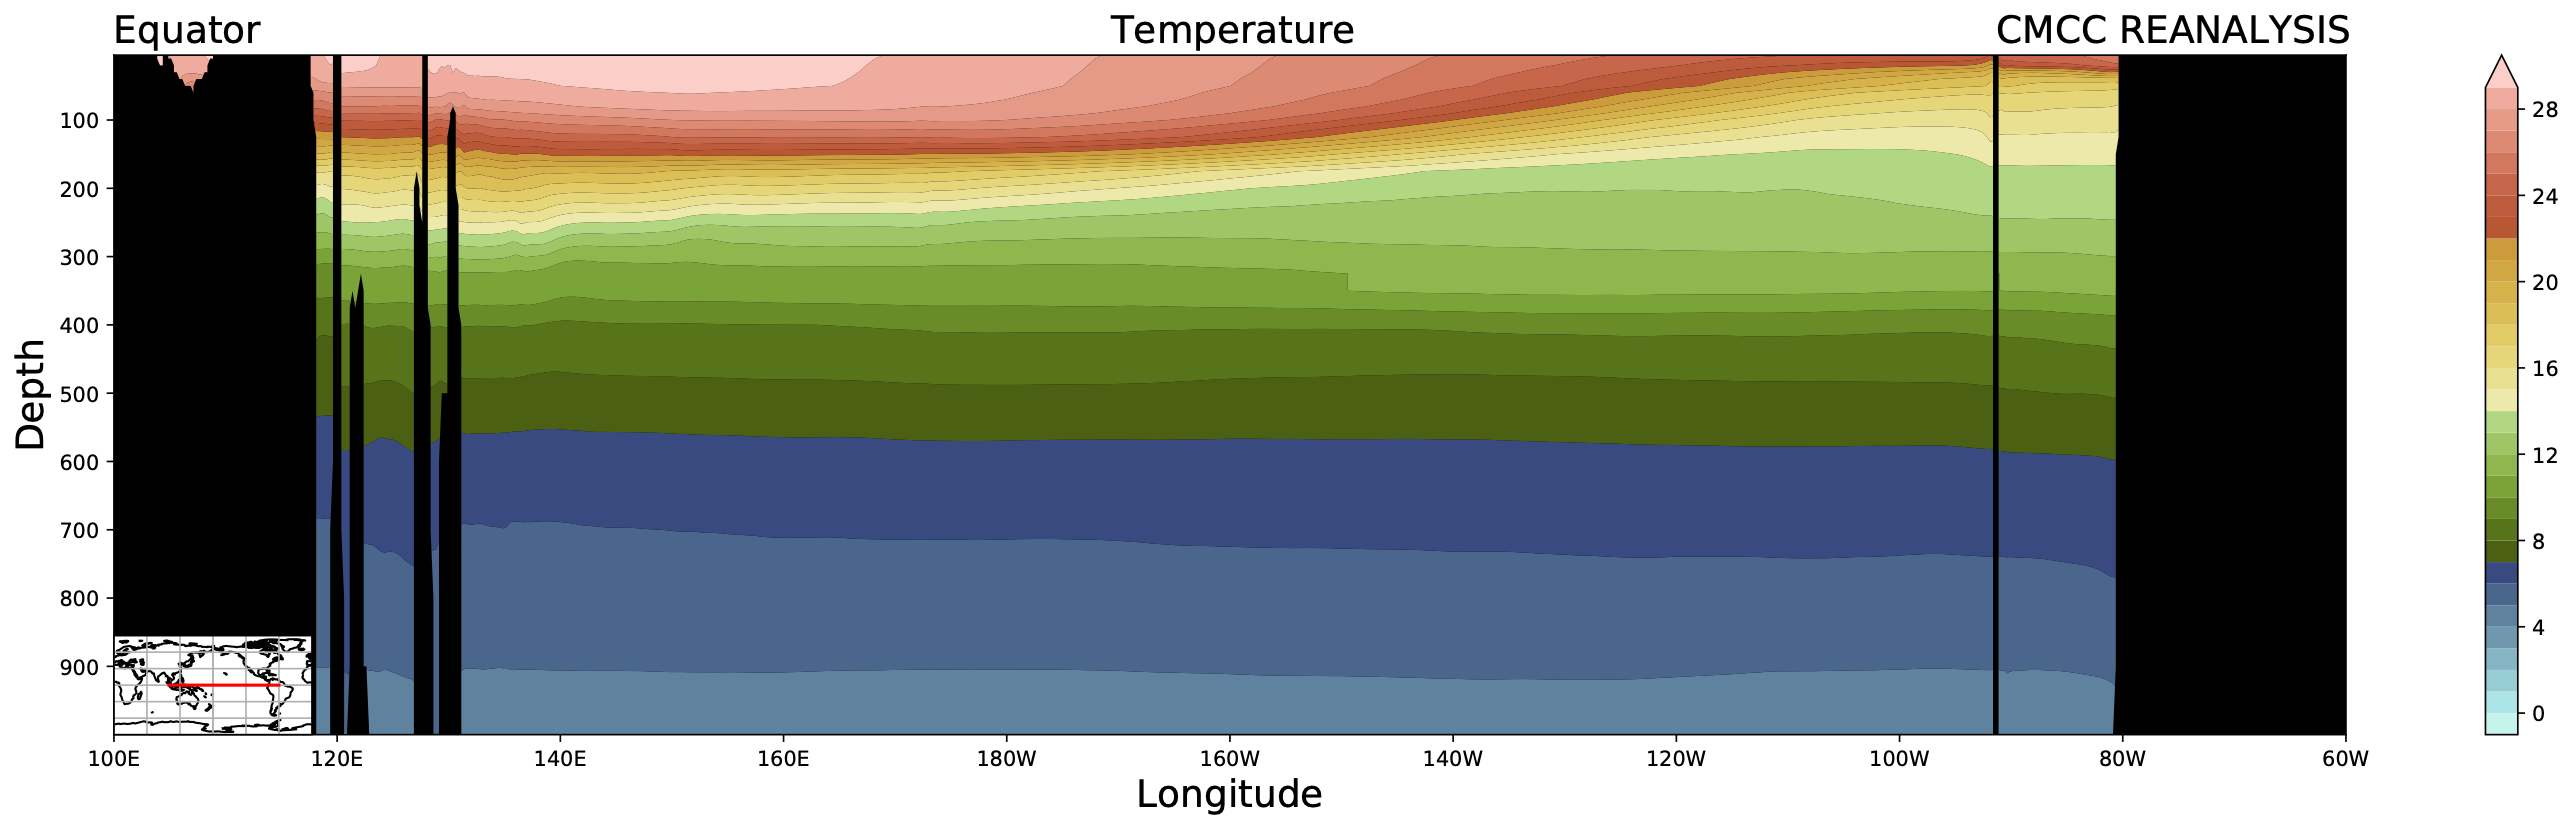
\includegraphics[width = .7 \textwidth]{figs/GD/SectEquator1000.png}
\caption{} \label{fig:}
\end{figure}

We can gain more insights in the equatorial structure by looking at a
longitudinal section along the Equator in the Pacific (Fig.
\texttt{fig:6103}). The thermocline is clearly visible, but there is a
clear east-west inclination of the thermocline with a significant
deepening in the West Pacific and a mush shallower layer in the East,
close to the South American coast. The thermal gradient is really strong
and it crosses several degrees in a few tens of meters.

\subsection{The salinity structure of the
Ocean}\label{the-salinity-structure-of-the-ocean}

The salinity structure of the oceans is shown in Fig. \texttt{fig:710}.
The top panel shows the salinity near the surface at a nominal depth of
5m. We notice that there is a complex structure with low salinity
(fresher) waters at the poles and progressively more saline water moving
towards the Equator, but then salinity decreases again at the equator.
It is probably instructive to look at the latitudinal distribution of
the precipitation (Fig. \texttt{fig:70a}). We can notice that the peaks
of precipitation in the midlatitude and at the Equator are correlated
with the low-salinity areas, whereas the subtropical regions are regions
of strong evaporation, whose signature is the high salinity of the
surface waters.

The Pacific Ocean is fresher than the Atlantic or even the Indian Ocean.
We can see from the map at 1000m that sources of saline waters are
marginal seas like the Mediterranean and the Persian Gulf. These areas
are evaporative basins that produce water so saline that it dominates
over the temperature effect and becomes denser so that we can find
Mediterranean water nelow the surface.

\begin{figure}
\centering
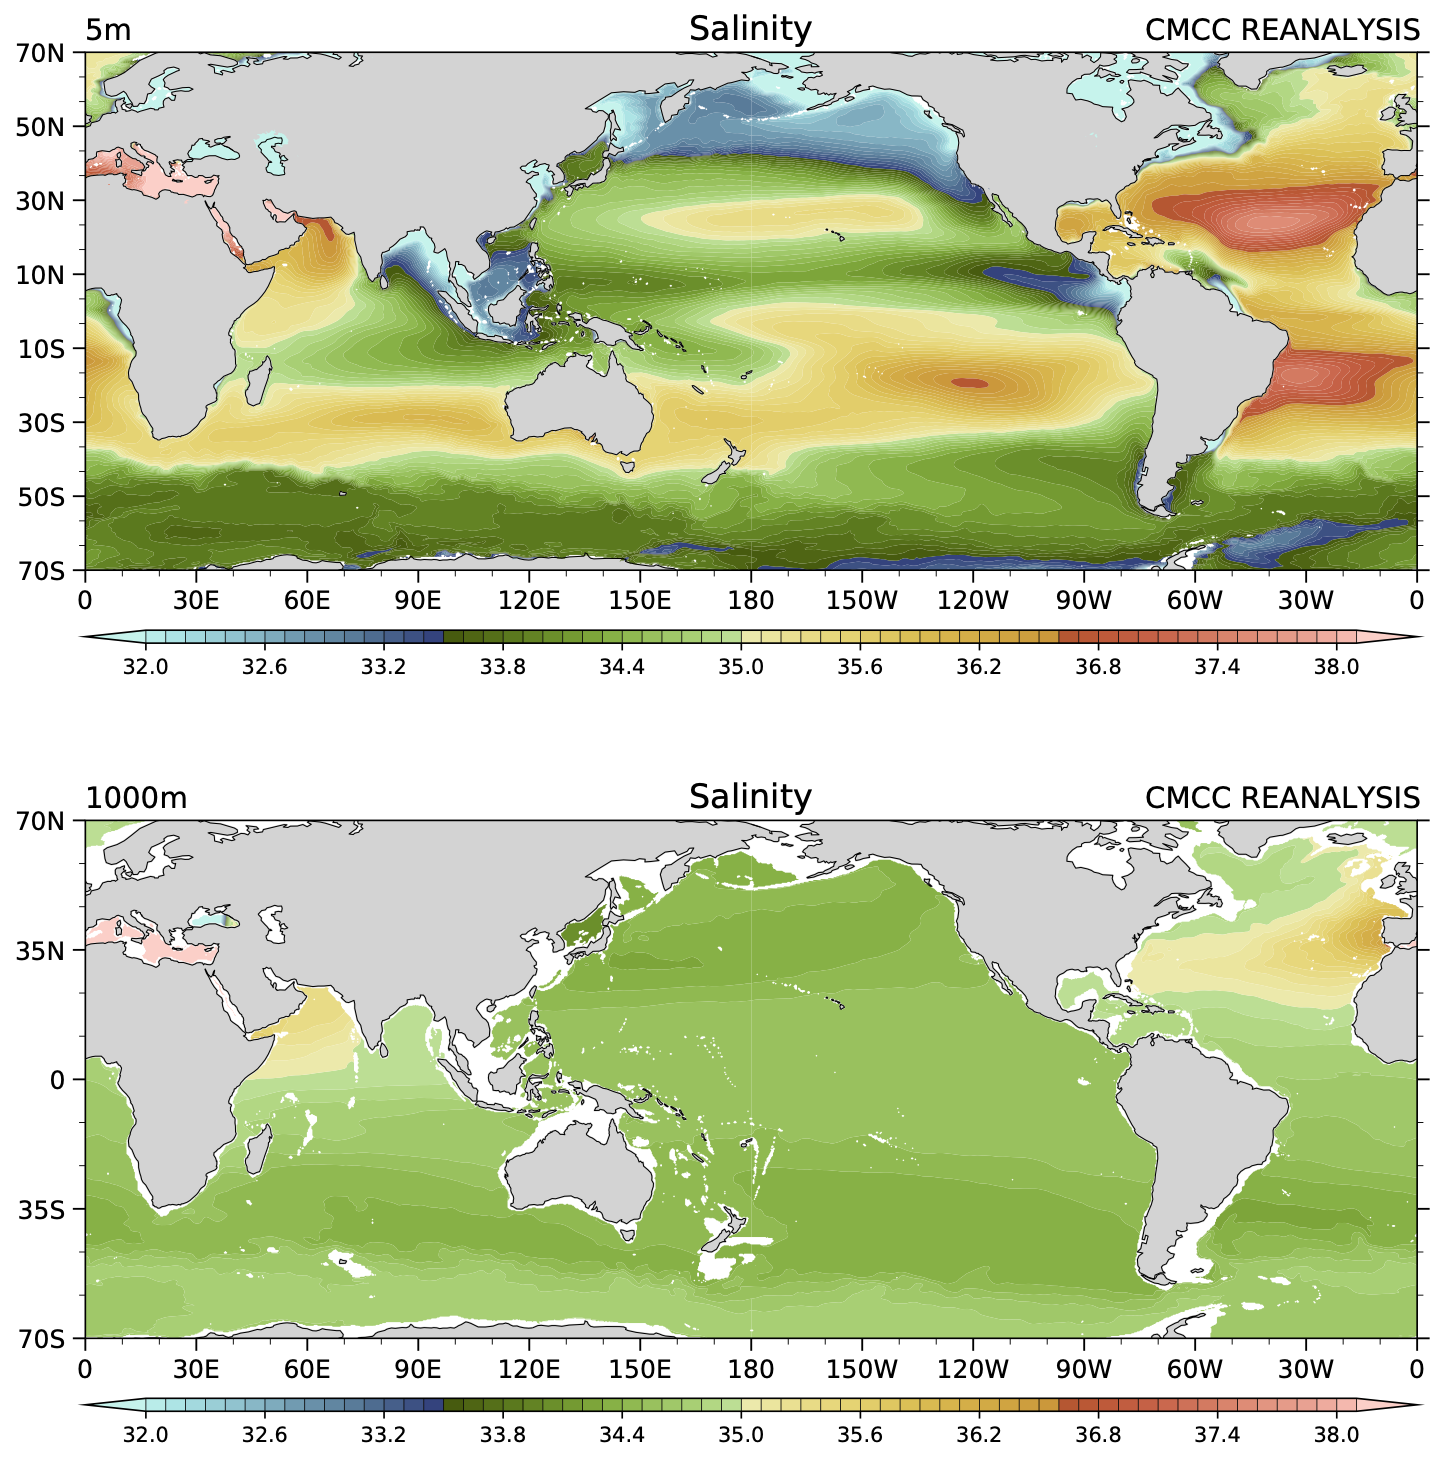
\includegraphics[width = .7 \textwidth]{figs/GD/Sal5-1000.png}
\caption{} \label{fig:}
\end{figure}

The effect of the precipitation is less visible at the deeper depth pf
1000m (bottom panel), where the ocean tends to be fresher and more
uniform. We are using here the same scale to give a feeling of the
changes in salinity, except for the Atlantic and the east Indian Ocean,
the salinity is around 34 psu. The situation does not change much lower
down (Fig. \texttt{fig:7110}).

The effect of the runoff from major river systems is visible along the
Atlantic coast of South America where the Amazon river discharges and in
the Bay of Bengal and around Indochina from the run-off the major rivers
there, the Ganges and the Mekong.

\begin{figure}
\centering
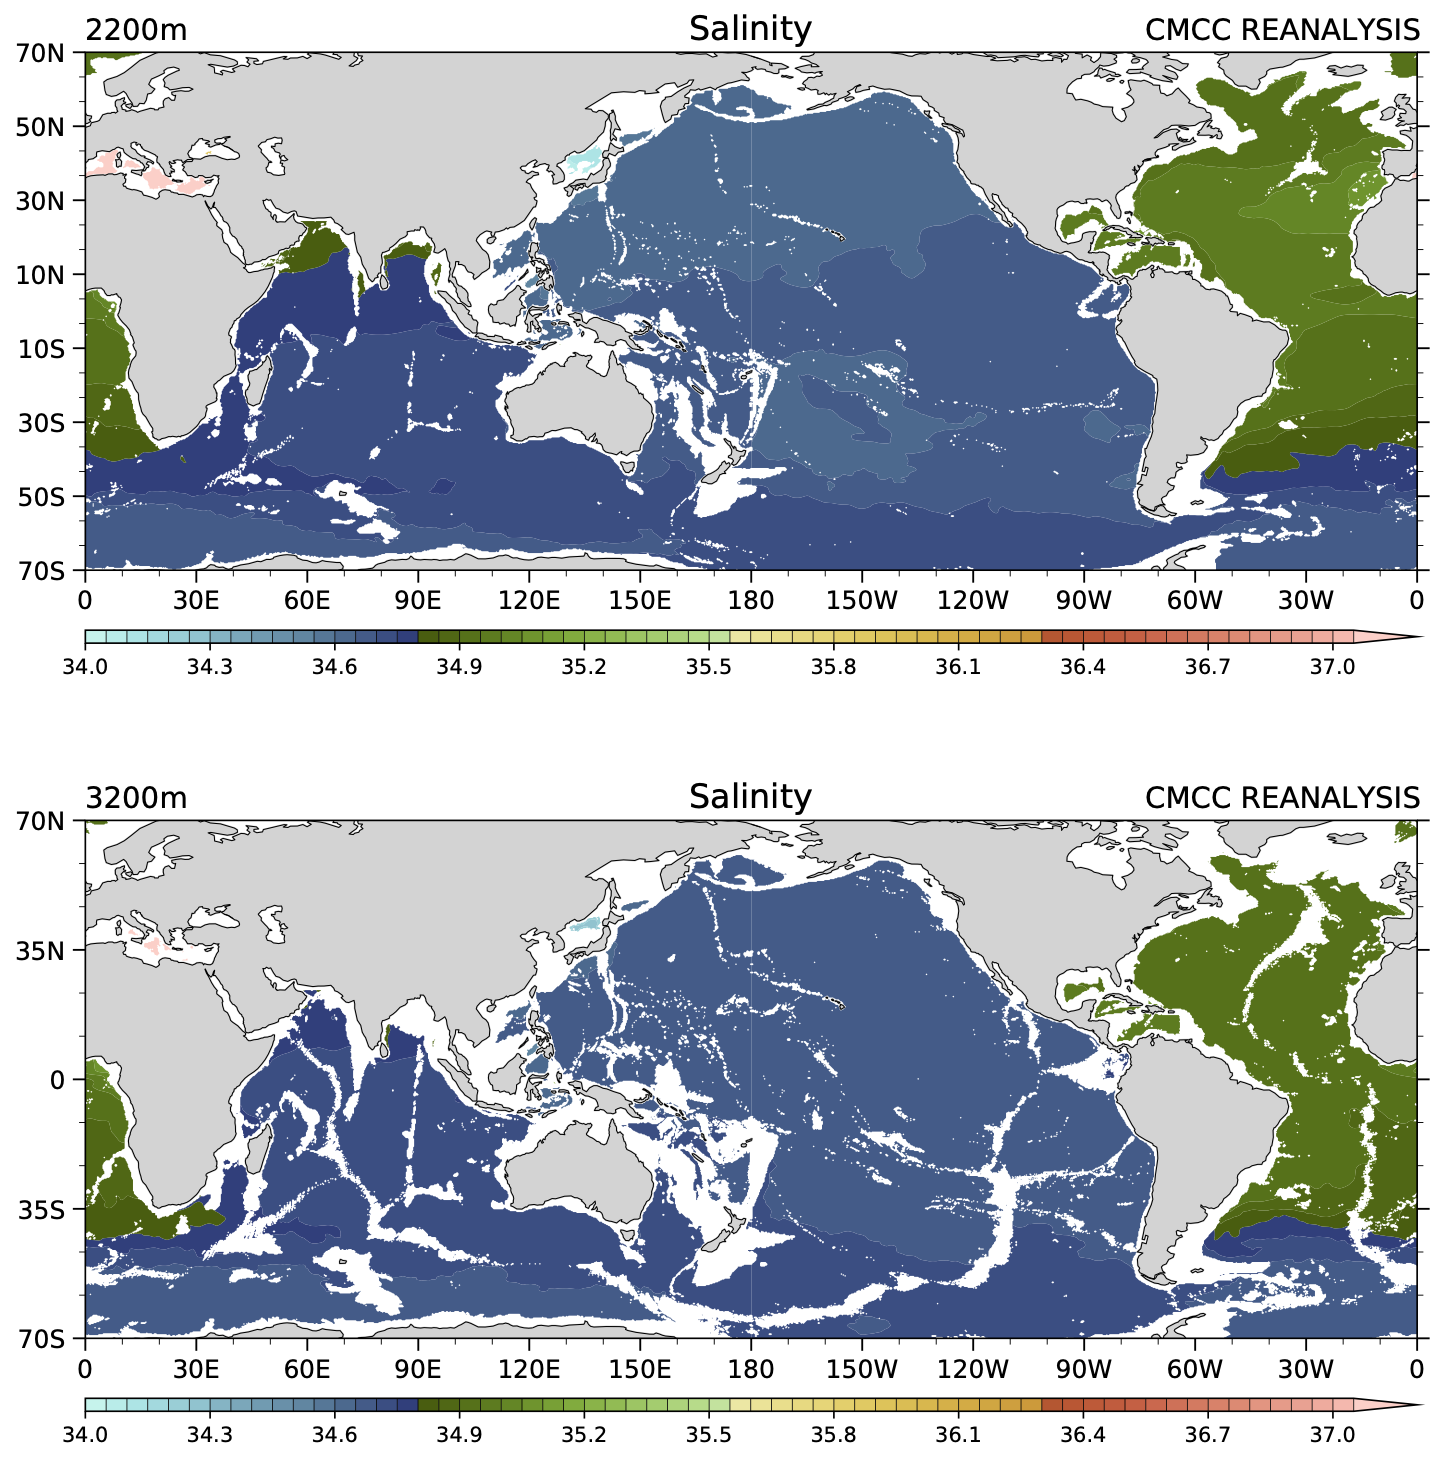
\includegraphics[width = .7 \textwidth]{figs/GD/Sal2200-3200.png}
\caption{} \label{fig:}
\end{figure}

Going even deeper (Fig. \texttt{fig:712}) we have to change drastically
the scale. The oceans are remarkably uniform and the salinity deviations
are really small.

\begin{figure}
\centering
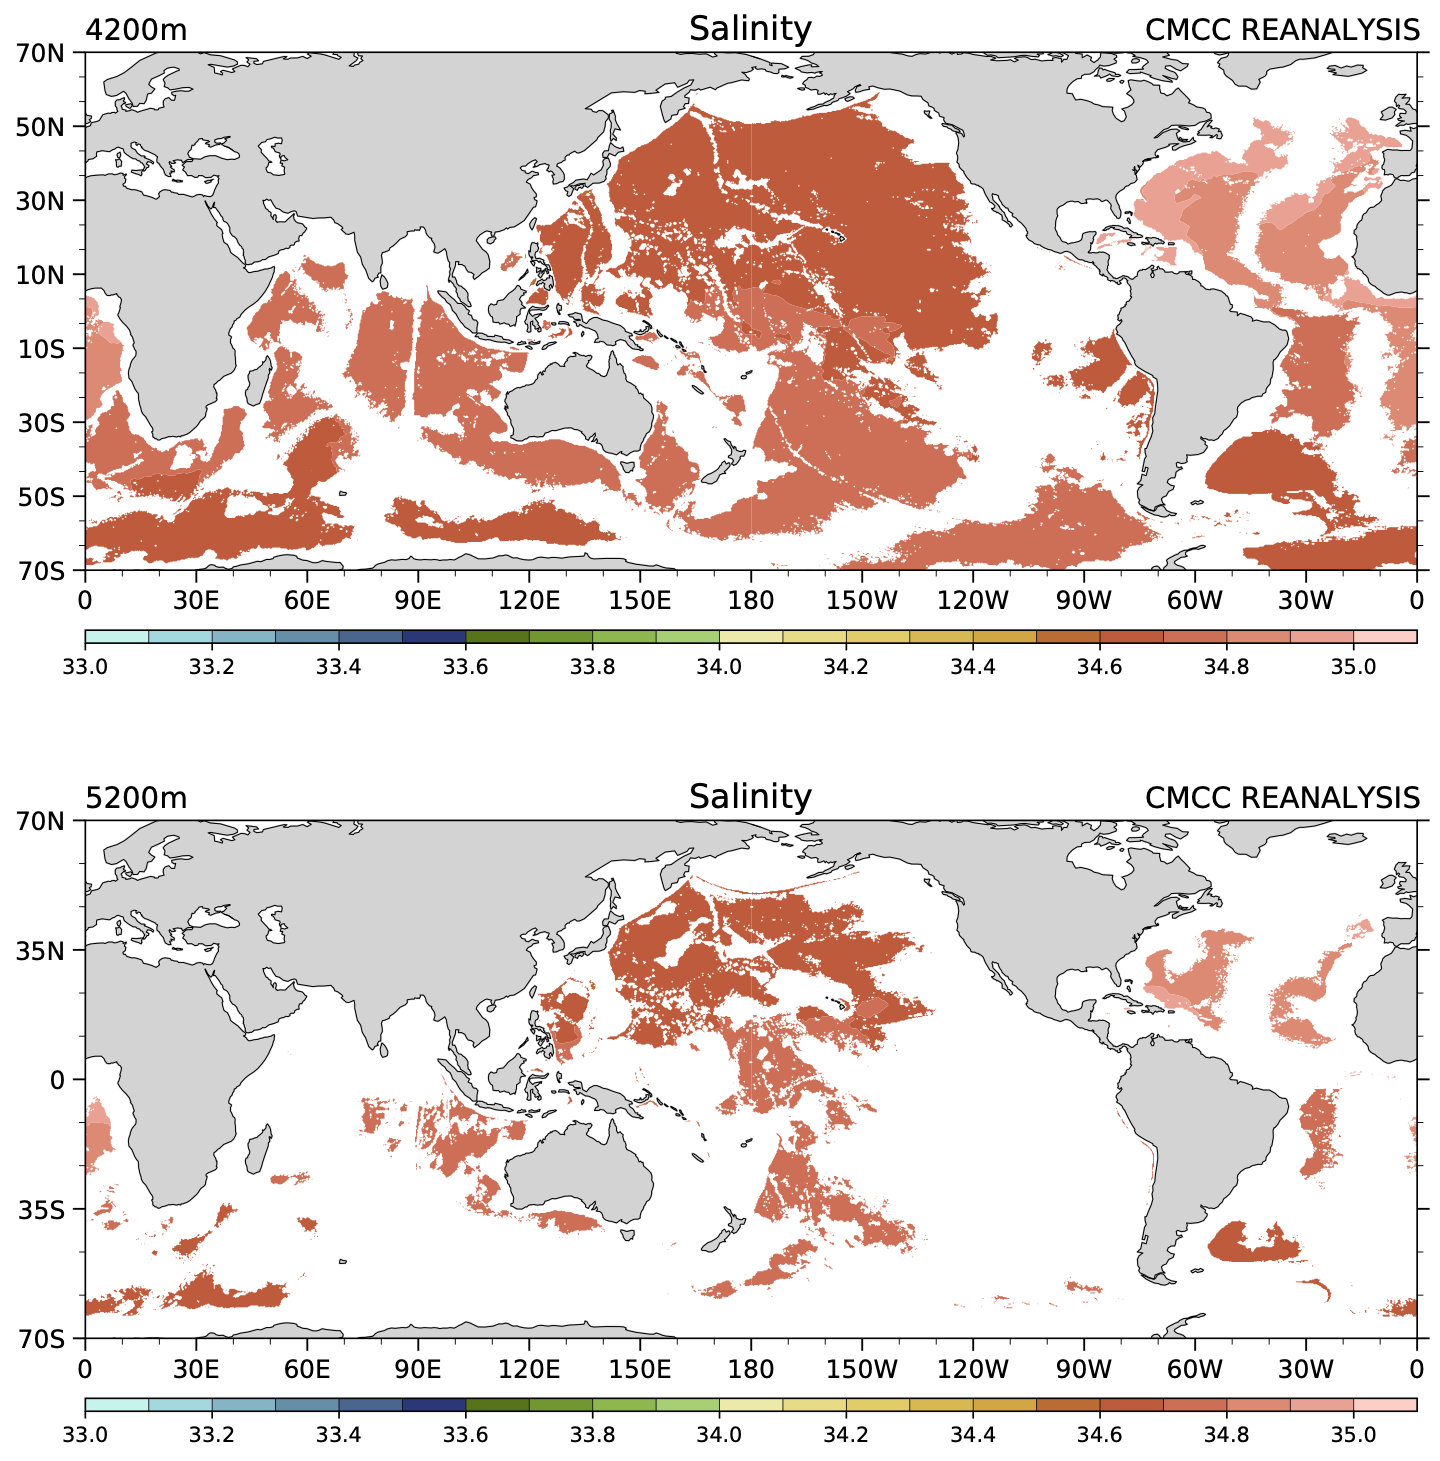
\includegraphics[width = .7 \textwidth]{figs/GD/Sal4200-5200.png}
\caption{} \label{fig:}
\end{figure}

Looking at the North Atlantic (Fig. \texttt{fig:713}) we notice that
there is a strong salinity gradient along the North American Coast that
follows roughly the pattern of the temperature gradient in Fig.
\texttt{fig:613}. Strong temperature gradients are presumably to be
connected to the existence of currents, but we will need to check the
density, depending on the salinity later, to be really sure. Anyway,
this picture is giving a strong indication of the existence of something
remarkable and intense along the western boundary of the Atlantic ocean.

\begin{figure}
\centering
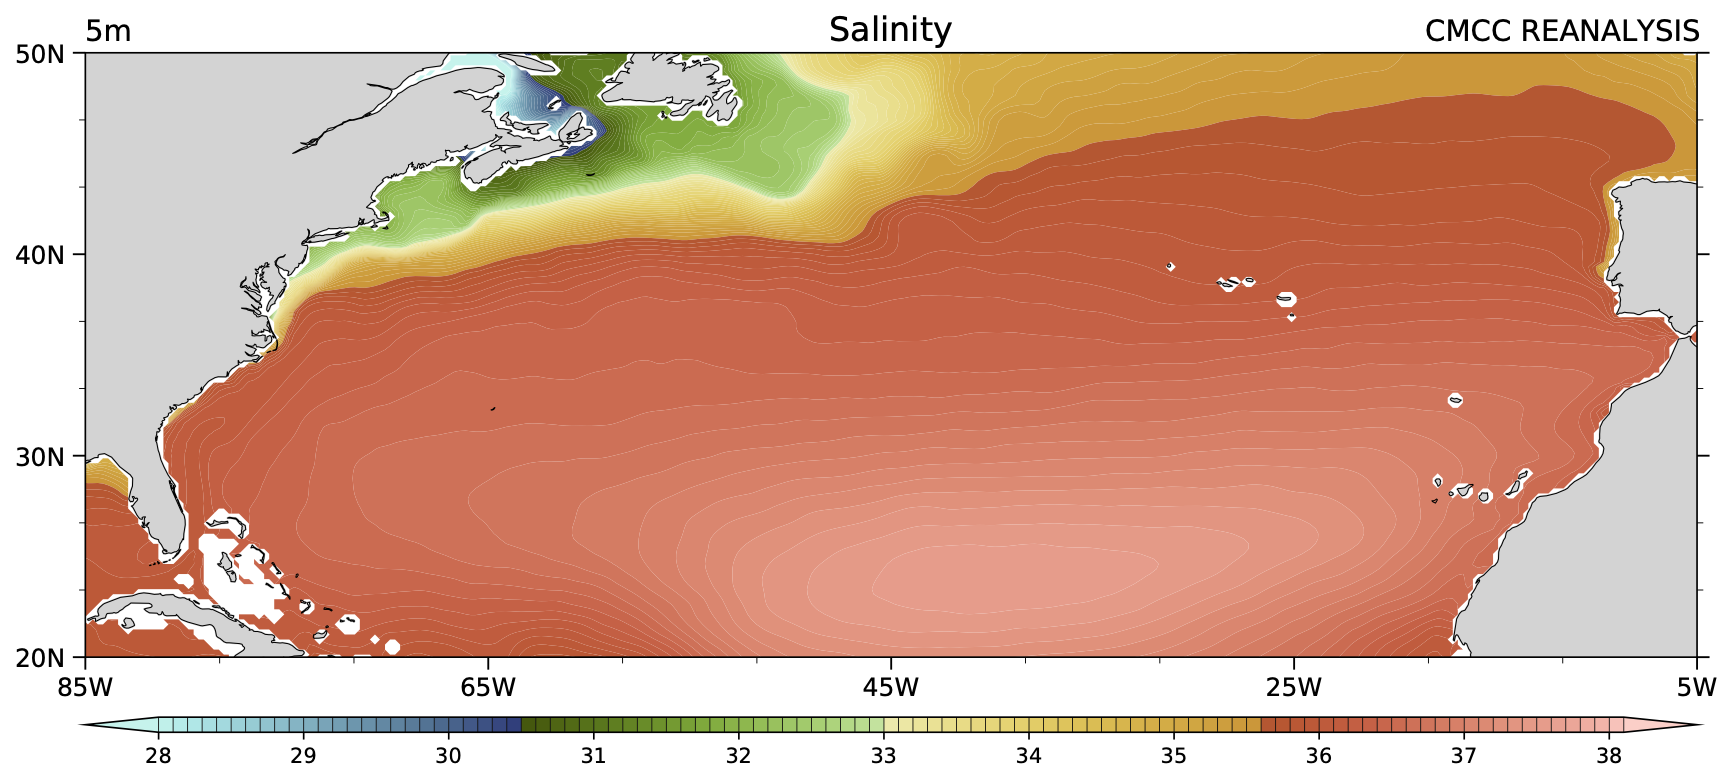
\includegraphics[width = .7 \textwidth]{figs/GD/SGulf5.png}
\caption{Northern Atlantic salinity for the ocean at 5m.}
\end{figure}

A similar situation exist in the North Pacific along the Japan coast and
therefore we can start to suspect that this has to do with the presence
of the continental boundary.

\begin{figure}
\centering
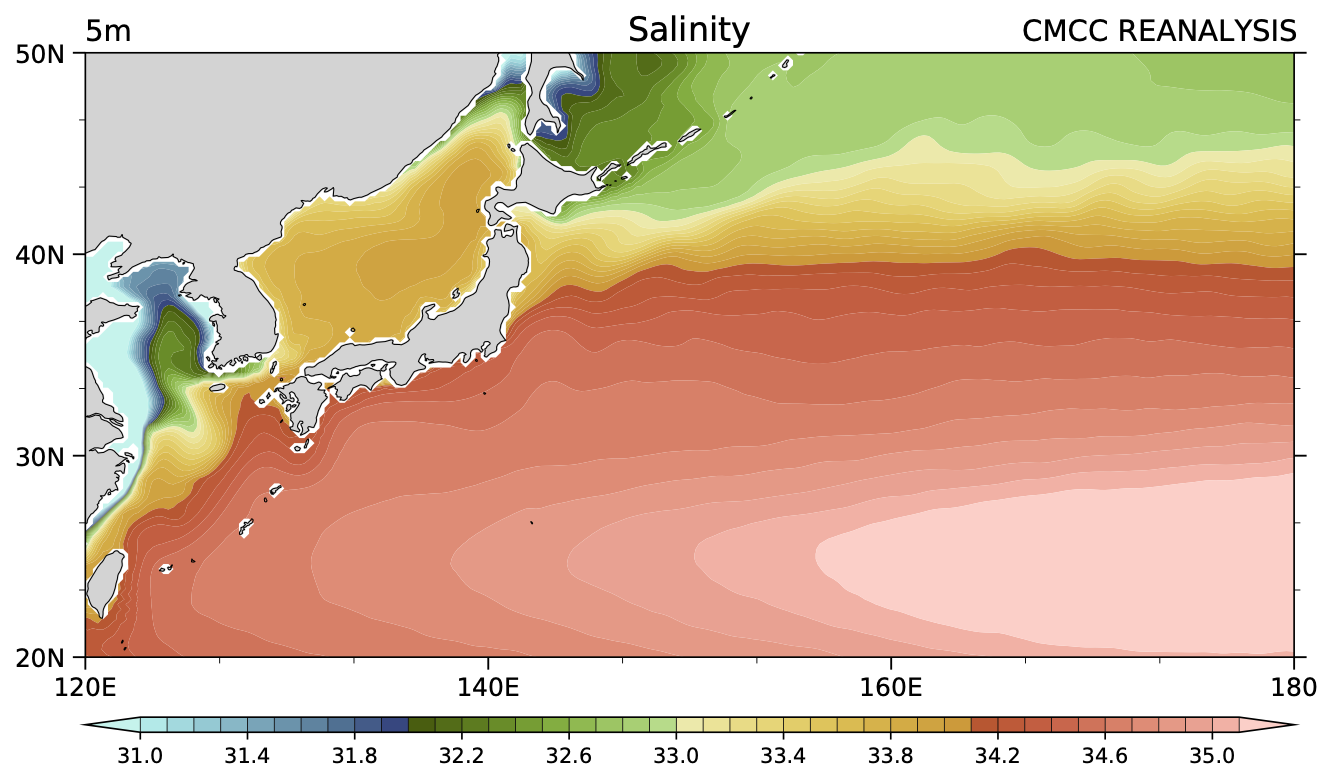
\includegraphics[width = .7 \textwidth]{figs/GD/SKur5.png}
\caption{Northern Pacific Salinity for the ocean at 5m.}
\end{figure}

The previous analysis of the temperature is giving us hints of a strong
vertical structure of the oceans, so it may be useful to look at the
vertical distribution somewhat more in detail. Fig. \texttt{fig:7100}
shows the same section North-South section of Fig. \texttt{fig:6100}
along the longitude of 25W, roughly in the middle of the Atlantic Ocean.
The salinity follows the a similar pattern as the temperature with a
strong gradient approximately at the thermocline, the high salinity is
confined in thin ;layers at the surface, but some interesting behaviour
is visible below. In the Northern Hemisphere we can see the
Mediterranean water penetrating at depth and actually protruding under
the fresher water of Antarctic origin that is colder, but because is
fresher floats over the Mediterranean water. Really cold Antarctic water
reaches the bottom, filling the abyssal plains of the basin.

\begin{figure}
\centering
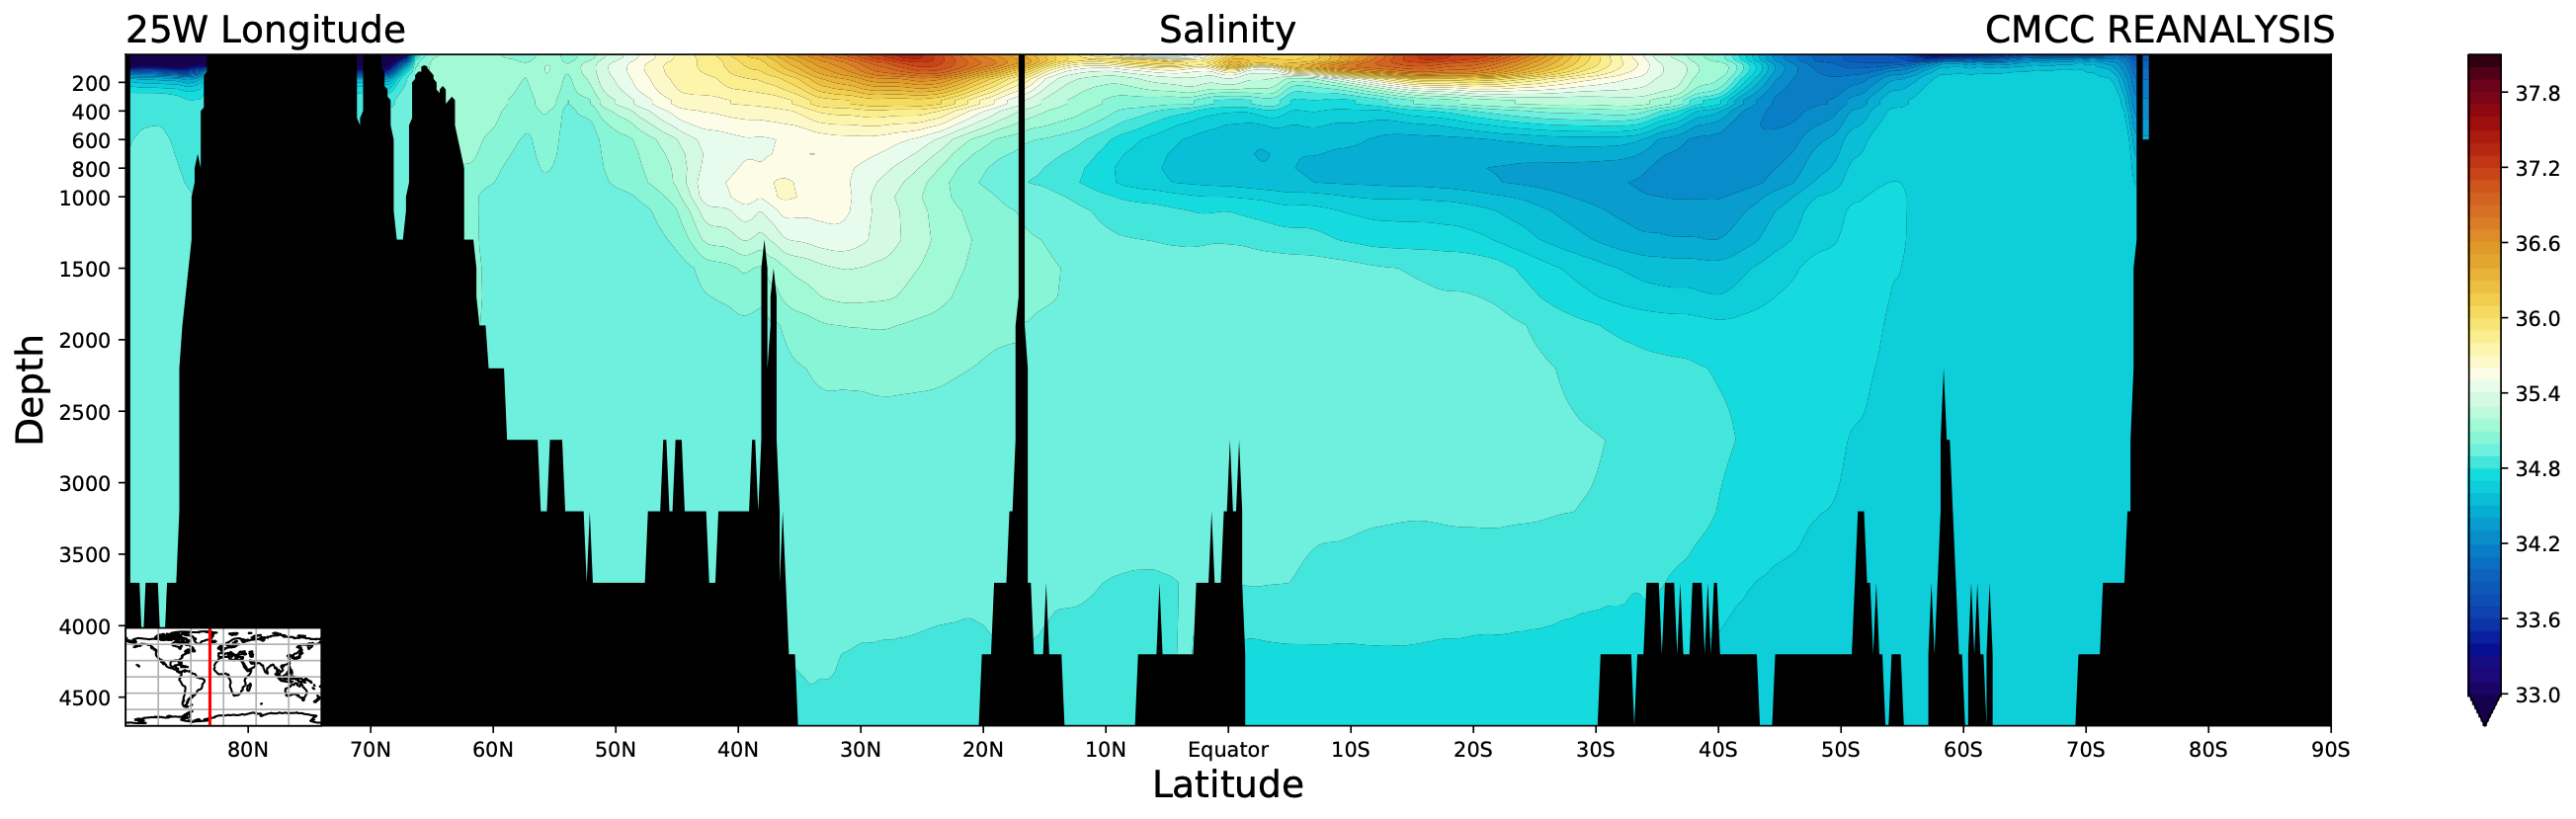
\includegraphics[width = .7 \textwidth]{figs/GD/SectSal25W5000.png}
\caption{North-South Salinity section at 25W longitude.}
\end{figure}

The Mediterranean waters are clearly visible in a longitude-depth
section (Fig. \texttt{fig:71000}). The saline mediterranean water sinks
to about 1000m because it is warmer than the Atlantic but much more
saline so it is denser and it reaches an equilibrium depth at about
1000m.

\begin{figure}
\centering
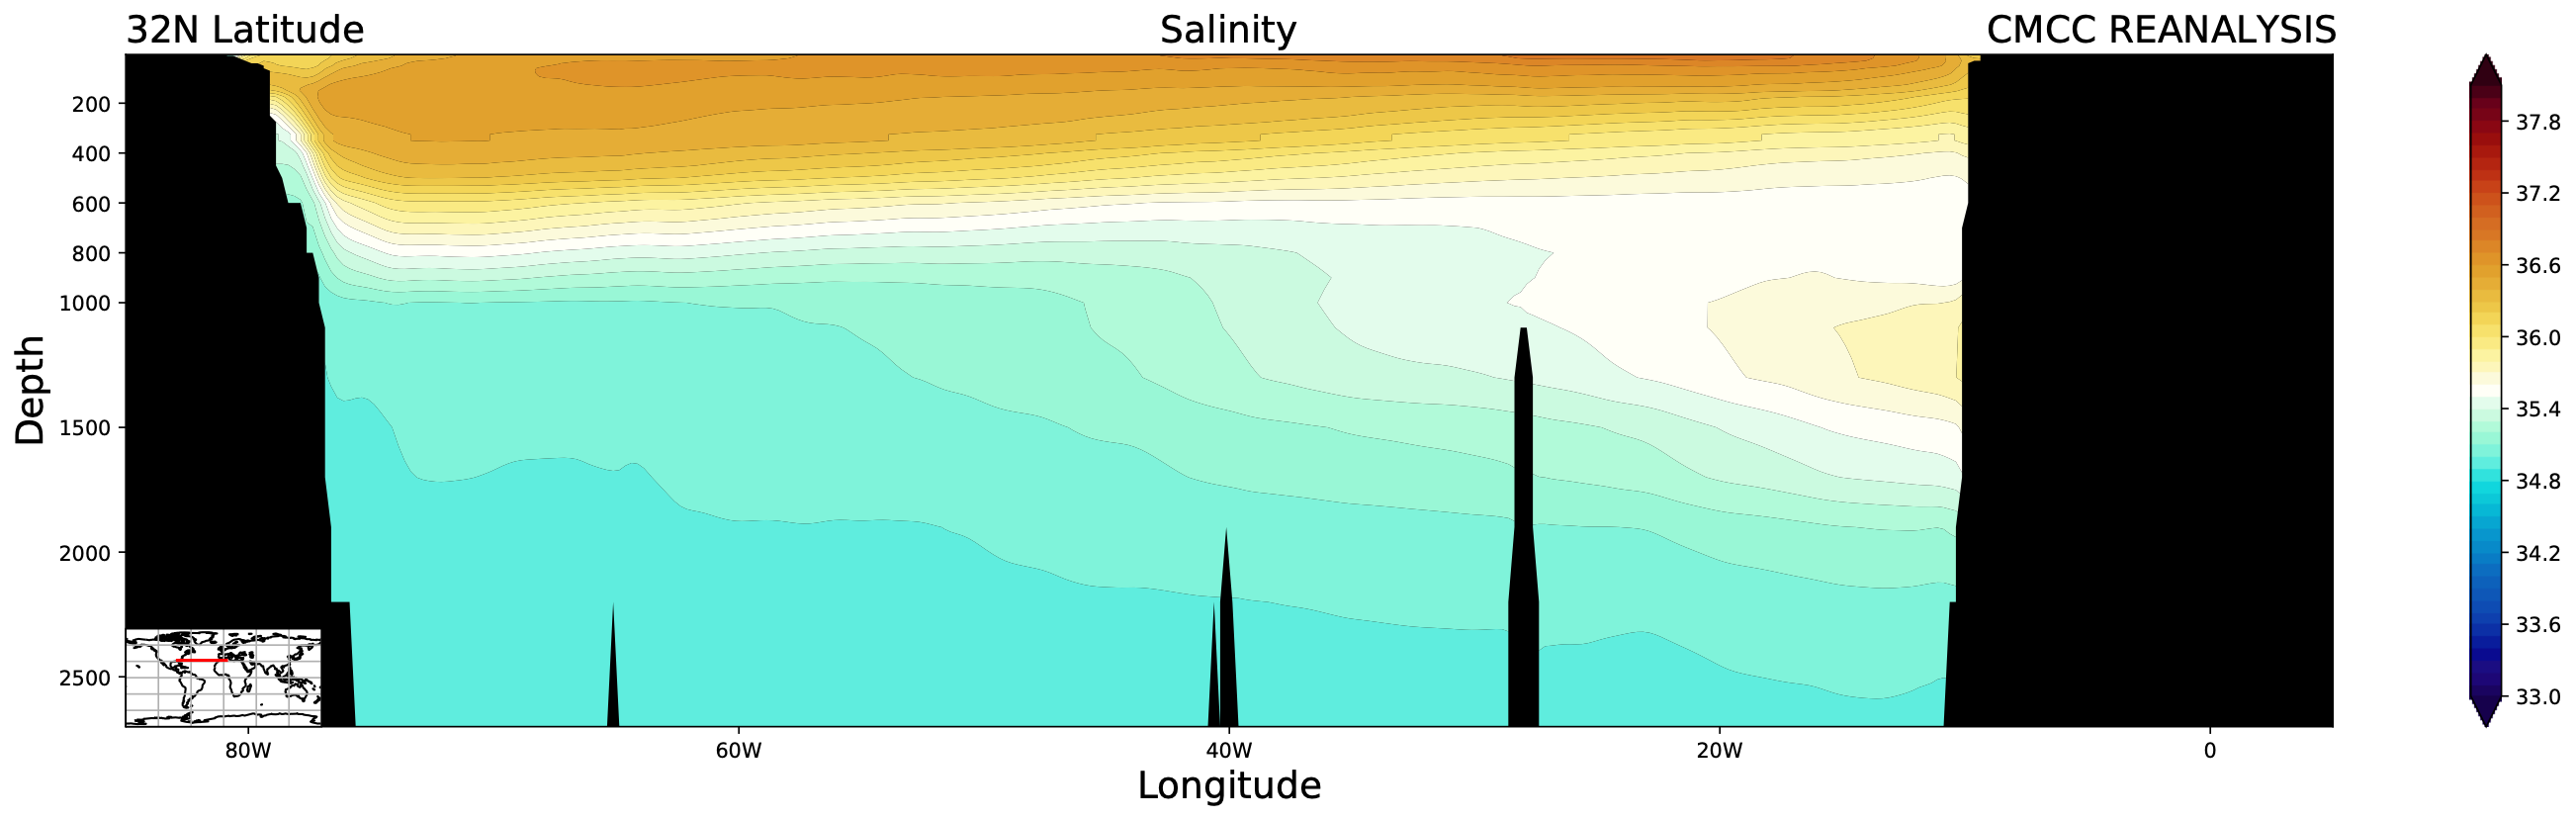
\includegraphics[width = .7 \textwidth]{figs/GD/SectSalinity32N3000.png}
\caption{Longitude depth section about 32N in the Atlantic Ocean.}
\end{figure}

\begin{figure}
\centering
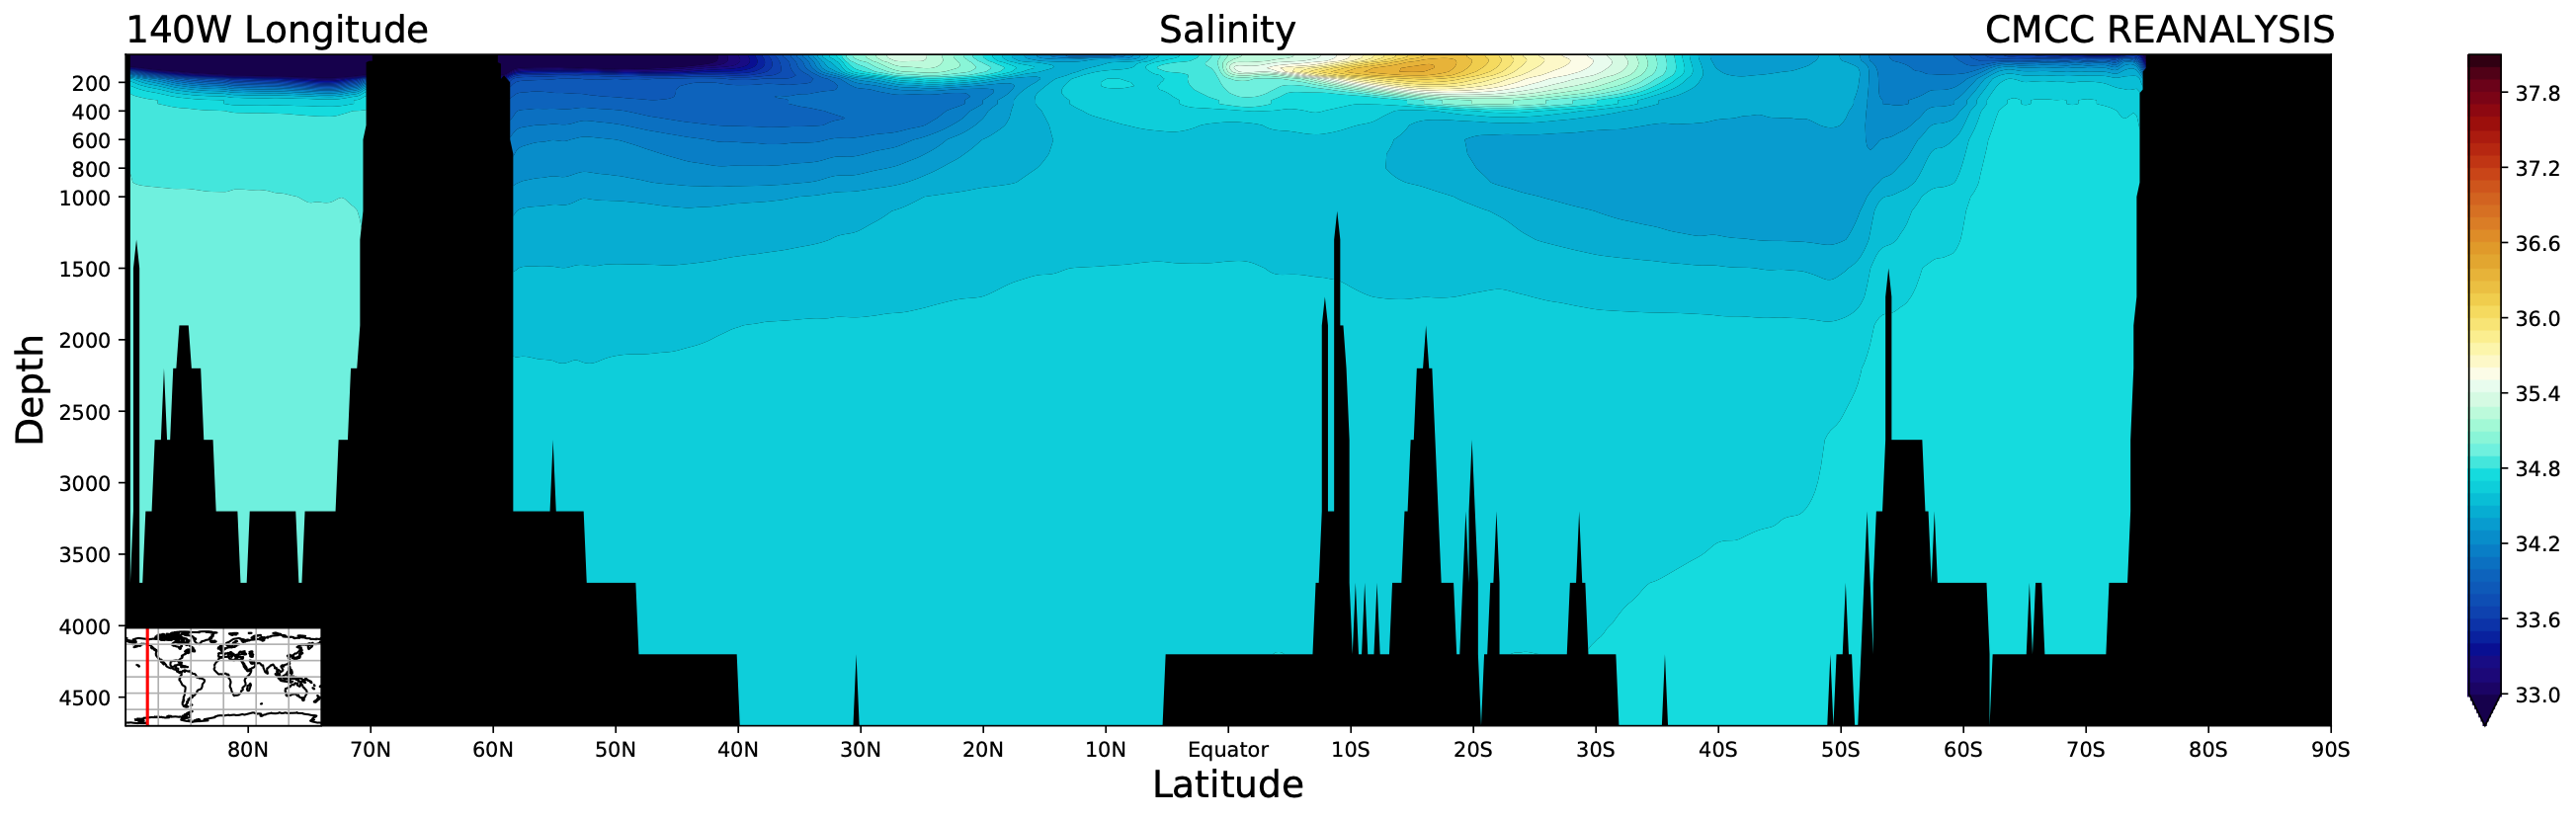
\includegraphics[width = .7 \textwidth]{figs/GD/SectSal140W5000.png}
\caption{As in Fig. \texttt{fig:7100} but for 140W longitude}
\end{figure}

The vertical structure of the Pacific Ocean (Fig. \texttt{fig:7101}) is
different and what we see is a situation where salinity is slowly
varying getting fresher toward the surface, with the thin saline water
in the subtropics a clear signature of the equatorial upwelling and the
Antarctic water filling the abyssal plains. The Indian Ocean is similar
to the Pacific South of the Equator but North of the Equator at this
longitude is fresher.

\begin{figure}
\centering
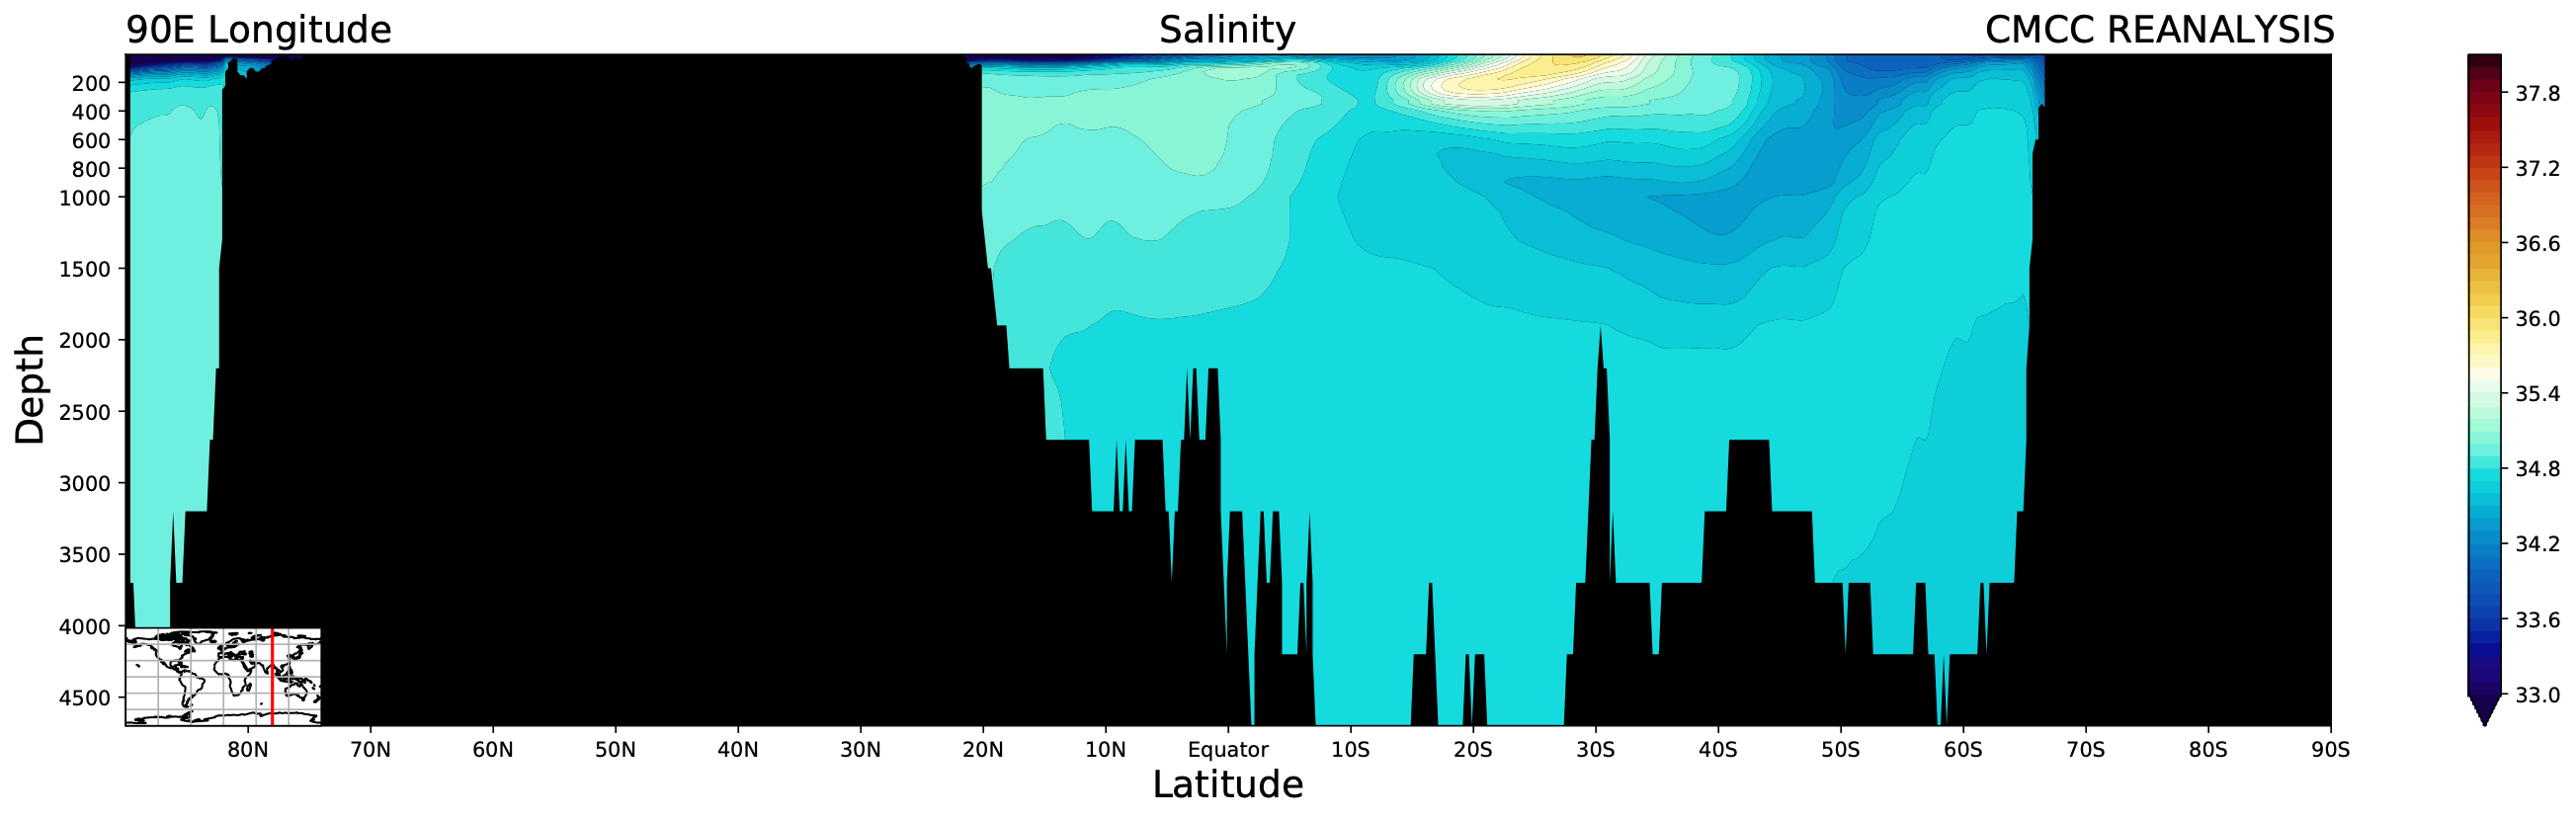
\includegraphics[width = .7 \textwidth]{figs/GD/SectSal90E5000.png}
\caption{As in Fig. \texttt{fig:7100} but for 90E longitude}
\end{figure}

The Indian Ocean (Fig. \texttt{fig:7102}) shown here as a section
cutting essentially through the Bay of Bengal, shows a similar strong
stratification, but there are only weak signs of an equatorial upwelling
of cold water.

\begin{figure}
\centering
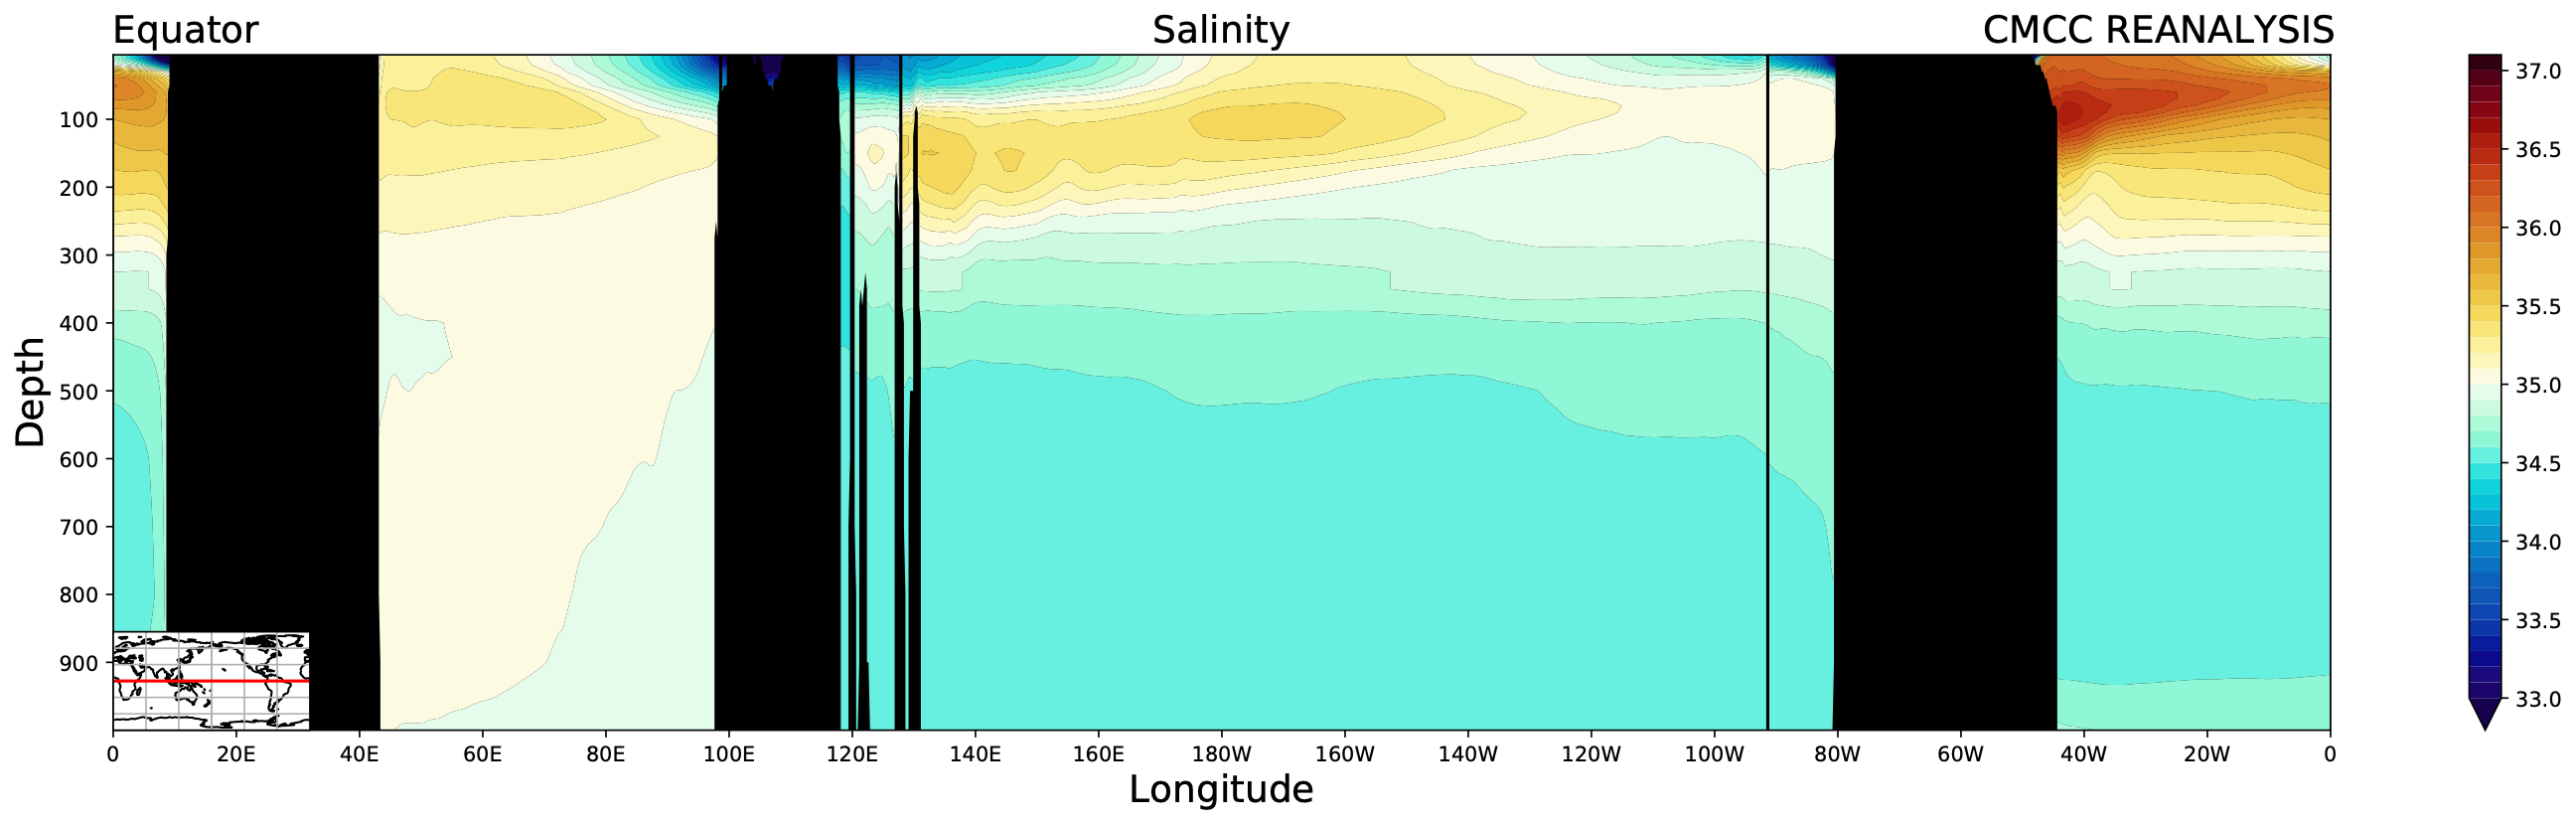
\includegraphics[width = .7 \textwidth]{figs/GD/SectSalinityEquator1000.png}
\caption{} \label{fig:}
\end{figure}

We can gain more insights in the equatorial structure by looking at a
longitudinal section along the Equator in the Pacific (Fig.
\texttt{fig:7103}). Here we see the general difference between the
Atlantic and the Pacific, but we also see that the salinity is following
the slant of the equatorial thermocline and the equatorial upwelling in
the East Pacific. The effect of the major precipitation center of ITCZ
in the West Pacific is visible in fresh water at the surface in the
West.

\subsection{Ocean Currents}\label{ocean-currents}

\subsubsection{The overall basin
circulation}\label{the-overall-basin-circulation}

The surface currents of the Atlantic ocean are shown in Fig.
\texttt{fig:8100}. As we might have suspected from the temperature
structure there is a strong northward current along the North American
coast that reaches all the way across the North Atlantic to Europe, the
Gulf Stream. Strong currents are also visible in the Equatorial area
where they connect to the mid-latitude circulation forming a large
circular system, the Subtropical Gyre. The South Atlantic has a similar
gyre in the subtropical region, but at higher latitudes we can notice a
strong westerly current cutting all along the basin, essentially along a
latitude line between 40S and 50S.

\begin{figure}
\centering
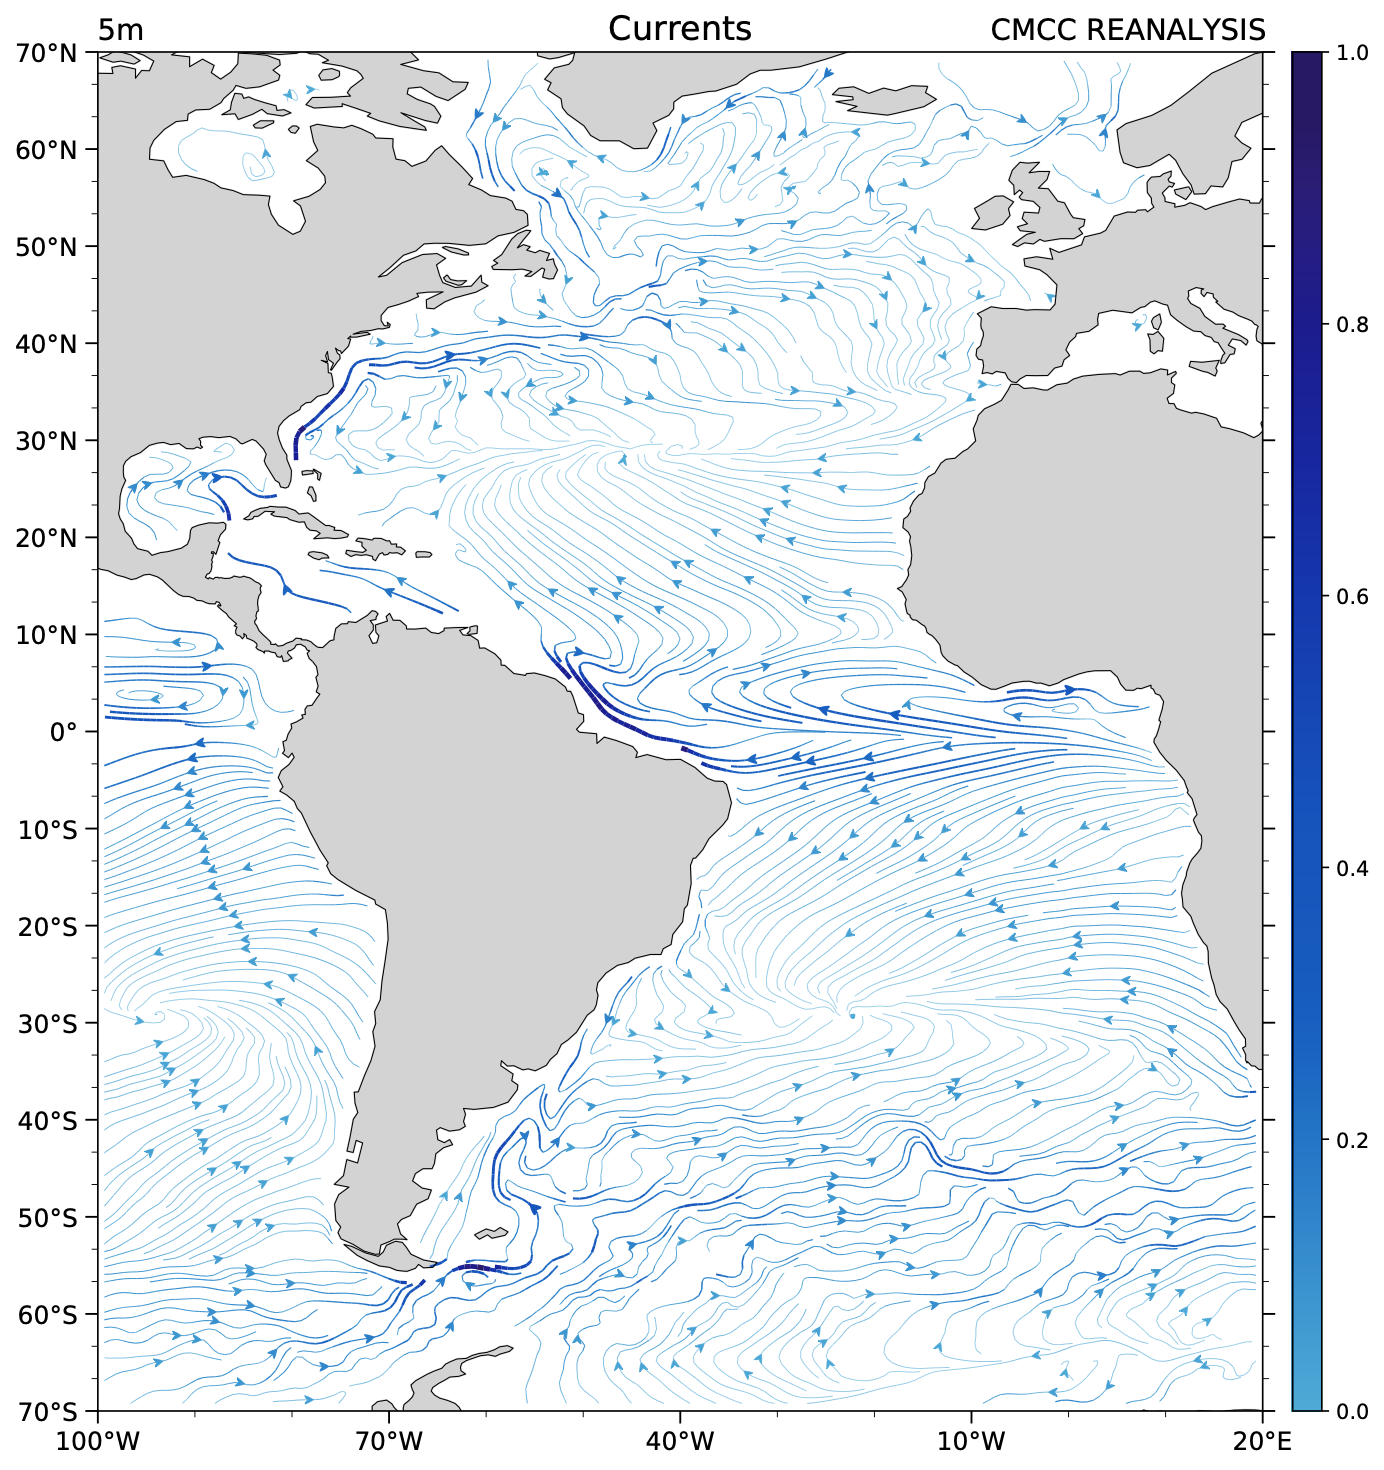
\includegraphics[width = .7 \textwidth]{figs/GD/UVstream5mGLOBNA.png}
\caption{} \label{fig:}
\end{figure}

The North Pacific surface circulation is shown in Fig.
\texttt{fig:8101}. We can notice here again a strong current along the
Western boundary of the basin that than feed into a basin wide gyre that
connects to the equatorial circulation. The boundary current, known her
as the Kuroshio Current, is very narrow and intense along the Japan
coast, as it is also the case of the Gulf Stream in the Atlantic, and it
tapers into a wide system of streams and eddies into the open ocean.

It is possible to see also local system, like the small gyre off the
Alaskan coast and similar circulation in the marginal seas, like the Sea
of Okhotsk, near the Siberian coast. Their presence is remarkable as we
are looking here at climatological averages over more than 40 years and
so they are stable and persistent features. This is another reminder of
how even relatively smaller feature in the ocean can be climatologically
persistent over many years.

\begin{figure}
\centering
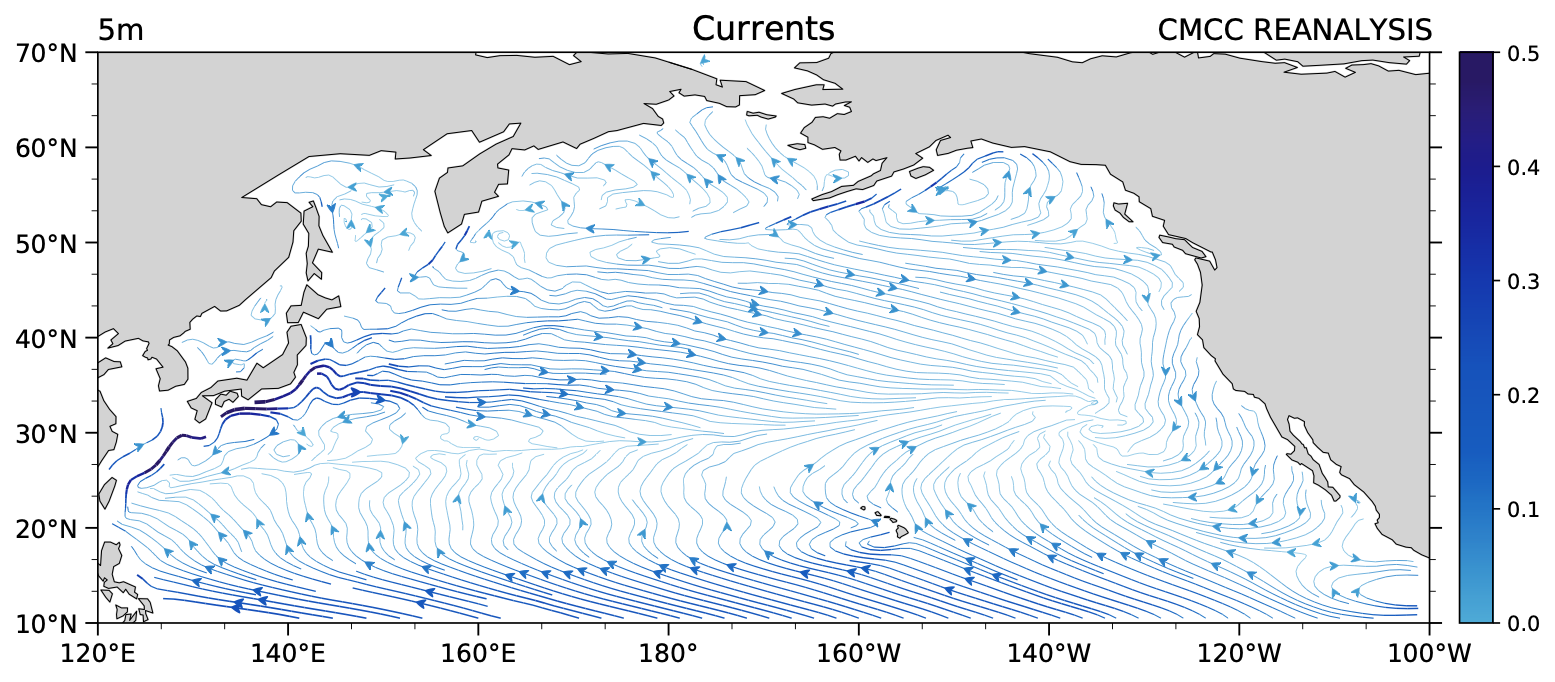
\includegraphics[width = .7 \textwidth]{figs/GD/UVstream5mGLOBNP.png}
\caption{} \label{fig:}
\end{figure}

The circulation of the South Pacific Ocean is shown in Fig.
\texttt{fig:8102}. The subtropical gyre is visible also here, but there
is a weak indication of a western intensification current in the West
pacific, close to the coasts of Australia and New Zealand. The strong
high latitude current that we have seen in the Atlantic is aldo present
here end evidently connect to the other basin through the Drake Passage,
that is the Straits between South America and Antarctica.

\begin{figure}
\centering
\includegraphics[width = .7 \textwidth]{figs/GD/UVstream5mGLOBSP.png}
\caption{} \label{fig:}
\end{figure}

The Indian Ocean circulation is shown in Fig. \texttt{fig:8103}. The
Indian Ocean is confined by continental masses in the north, so it is
mostly composed of the equatorial region and the midlatitudes are all in
the Southern Hemisphere. The subtropical gyre is present, together with
features North of Madagascar. A boundary current develops on the African
coast, The westerly current in the southern mid-latitudes is visible
also here, strong and with a vigorous eddy field.

\begin{figure}
\centering
\includegraphics[width = .7 \textwidth]{figs/GD/UVstream5mGLOBIND.png}
\caption{} \label{fig:}
\end{figure}

At this point we can suspect that there is probably a continuous ring of
currents around Antarctica and this can be confirmed by the bottom panel
of Fig. \texttt{fig:8103} that shows the entire extent around a
longitude circle of the current, known as the Antarctic Circumpolar
Current. It is a strong, highly turbulent system that connects all the
Ocean Basins.

\subsubsection{The equatorial
circulation}\label{the-equatorial-circulation}

The Equator is a special place for the atmosphere and so it is a special
place also for the Oceans. The circulation in this area is strongly
coupled with the atmospheric circulation and it is often characterized
by both westerly and easterly currents and by special behaviours right
at the Equator line. Futhermore, it is also very different from ocean to
ocean.

The equatorial current system in the Pacific Ocean is shown in Fig.
\texttt{fig:8106}. It is a complex system composed of two easterly
currents, the North and South Equatorial currents, sandwiching the
westerly Equatorial countercurrent. It is possible to notice that at the
Equator the currents are strongly easterly and diverging, leading to the
emergence of upwelling at the Equator by Ekman transport.

\begin{figure}
\centering
\includegraphics[width = .7 \textwidth]{figs/GD/UVstream5mPac.png}
\caption{} \label{fig:}
\end{figure}

The complexity of the equatorial current system can be further
appreciated by looking at the vertical section of the zonal current at
the Equator (Fig. \texttt{fig:8107}) A strong westerly current below the
surface, slanting from the West Pacific to the East Pacific, is visible
at depth between 200 and 300m. The speed is in excess of 1 m/s and it
gets progressively shallower in the East.

It is however part of an alternation of westerly and easterly currents
that become progressively weaker as they get deeper. They are centered
almost perfectly at the Equator, as it can be seen in Fig.
\texttt{fig:8108}. The latitudinal position of the undercurrent is very
tightly controlled by rotational effects and it precisely tracks the
position of the equatorial line.

\begin{figure}
\centering
\includegraphics[width = .7 \textwidth]{figs/GD/SectZonal_CurrentEquator1000.png}
\caption{} \label{fig:}
\end{figure}

The equatorial Atlantic Ocean surface circulation (Fig.
\texttt{fig:8109}). It is possible to see the easterly South Equatorial
Current that is straddling the Equator between 5S and 5N. The North
equatorial Countercurrent is westerly and it covers the area between 5N
and 10N, and the weaker North Equatorial Current is located at northern
latitudes. The equatorial flow is divergent and also in this case we can
presume the existence of upwelling at the Equator. A strong coastal
current is visible as the Guinea Current, in the Gulf of Guinea. The
South Equatorial Current feeds into the North Brazilian Current that
then flows northward along the South America coast, taking different
names as it finally emerges as the Caribbean Current in the Caribbean
sea.

A similar structure of alternating westerly and easterly undercurrents
exist also in the equatorial Atlantic (Fig. \texttt{fig:8108}), but it
is weaker and only the first westerly maximum is well visible. It is
also slanting towards the East, but the maximum is reached more towards
the western boundary of the basin with respect to the Pacific Ocean. The
deeper easterly jets are also much less weaker. The undercurrents jets
are essentially absent in the Indian Ocean.

\begin{figure}
\centering
\includegraphics[width = .7 \textwidth]{figs/GD/SectZonal_Current160W1000.png}
\caption{} \label{fig:}
\end{figure}

\begin{figure}
\centering
\includegraphics[width = .7 \textwidth]{figs/GD/UVstream5mATLEQ.png}
\caption{} \label{fig:}
\end{figure}

\subsubsection{The Gulf Stream}\label{the-gulf-stream}

The current system of the Gulf Stream is one of the major feature of the
global ocean circulation. It is shown in Fig.

\begin{figure}
\centering
\includegraphics[width = .7 \textwidth]{figs/GD/UVstream5mATLCARIB.png}
\caption{} \label{fig:}
\end{figure}

\begin{figure}
\centering
\includegraphics[width = .7 \textwidth]{figs/GD/UVstream800mATLCARIB.png}
\caption{As in Fig. \texttt{fig:8110aa}, but at 800m depth.}
\end{figure}

\begin{figure}
\centering
\includegraphics[width = .7 \textwidth]{figs/GD/UVstream1100mATLCARIB.png}
\caption{As in Fig. \texttt{fig:8110aa}, but at 1100m depth.}
\end{figure}

\begin{figure}
\centering
\includegraphics[width = .7 \textwidth]{figs/GD/UVstream1700mATLCARIB.png}
\caption{As in Fig. \texttt{fig:8110aa}, but at 1700m depth.}
\end{figure}

\subsubsection{The Kuroshio}\label{the-kuroshio}

The current system of the Kuroshio is one of the major feature of the
global ocean circulation. It is shown in Fig.

\begin{figure}
\centering
\includegraphics[width = .7 \textwidth]{figs/GD/UVstream5mKur.png}
\caption{} \label{fig:}
\end{figure}

\begin{figure}
\centering
\includegraphics[width = .7 \textwidth]{figs/GD/UVstream800mKUR.png}
\caption{As in Fig. \texttt{fig:8111aa}, but at 800m depth.}
\end{figure}

\begin{figure}
\centering
\includegraphics[width = .7 \textwidth]{figs/GD/UVstream1100mKUR.png}
\caption{As in Fig. \texttt{fig:8111aa}, but at 1100m depth.}
\end{figure}

\begin{figure}
\centering
\includegraphics[width = .7 \textwidth]{figs/GD/UVstream1700mKUR.png}
\caption{As in Fig. \texttt{fig:8111aa}, but at 1700m depth.}
\end{figure}

\subsubsection{The upwelling zones}\label{the-upwelling-zones}

\begin{figure}
\centering
\includegraphics[width = .7 \textwidth]{figs/GD/UVstream5mSATemp.png}
\caption{} \label{fig:}
\end{figure}

\begin{figure}
\centering
\includegraphics[width = .7 \textwidth]{figs/GD/UVstream5mAFRemp.png}
\caption{} \label{fig:}
\end{figure}

\subsubsection{The Somali Current}\label{the-somali-current}

\begin{figure}
\centering
\includegraphics[width = .7 \textwidth]{figs/GD/UVvec5mSOMSUM.png}
\caption{} \label{fig:}
\end{figure}

\begin{figure}
\centering
\includegraphics[width = .7 \textwidth]{figs/GD/UVvec5mSOMWIN.png}
\caption{As in Fig. \texttt{fig:8113a}, but for Summer.}
\end{figure}


    \printbibliography

\end{document}